% uWaterloo Thesis Template for LaTeX 
% Last Updated June 14, 2017 by Stephen Carr, IST Client Services
% FOR ASSISTANCE, please send mail to rt-IST-CSmathsci@ist.uwaterloo.ca

% Effective October 2006, the University of Waterloo 
% requires electronic thesis submission. See the uWaterloo thesis regulations at
% https://uwaterloo.ca/graduate-studies/thesis.

% DON'T FORGET TO ADD YOUR OWN NAME AND TITLE in the "hyperref" package
% configuration below. THIS INFORMATION GETS EMBEDDED IN THE PDF FINAL PDF DOCUMENT.
% You can view the information if you view Properties of the PDF document.

% Many faculties/departments also require one or more printed
% copies. This template attempts to satisfy both types of output. 
% It is based on the standard "book" document class which provides all necessary 
% sectioning structures and allows multi-part theses.

% DISCLAIMER
% To the best of our knowledge, this template satisfies the current uWaterloo requirements.
% However, it is your responsibility to assure that you have met all 
% requirements of the University and your particular department.
% Many thanks for the feedback from many graduates that assisted the development of this template.

% -----------------------------------------------------------------------

% By default, output is produced that is geared toward generating a PDF 
% version optimized for viewing on an electronic display, including 
% hyperlinks within the PDF.
 
% E.g. to process a thesis called "mythesis.tex" based on this template, run:

% pdflatex mythesis	-- first pass of the pdflatex processor
% bibtex mythesis	-- generates bibliography from .bib data file(s)
% makeindex         -- should be run only if an index is used 
% pdflatex mythesis	-- fixes numbering in cross-references, bibliographic references, glossaries, index, etc.
% pdflatex mythesis	-- fixes numbering in cross-references, bibliographic references, glossaries, index, etc.

% If you use the recommended LaTeX editor, Texmaker, you would open the mythesis.tex
% file, then click the PDFLaTeX button. Then run BibTeX (under the Tools menu).
% Then click the PDFLaTeX button two more times. If you have an index as well,
% you'll need to run MakeIndex from the Tools menu as well, before running pdflatex
% the last two times.

% N.B. The "pdftex" program allows graphics in the following formats to be
% included with the "\includegraphics" command: PNG, PDF, JPEG, TIFF
% Tip 1: Generate your figures and photos in the size you want them to appear
% in your thesis, rather than scaling them with \includegraphics options.
% Tip 2: Any drawings you do should be in scalable vector graphic formats:
% SVG, PNG, WMF, EPS and then converted to PNG or PDF, so they are scalable in
% the final PDF as well.
% Tip 3: Photographs should be cropped and compressed so as not to be too large.

% To create a PDF output that is optimized for double-sided printing: 
%
% 1) comment-out the \documentclass statement in the preamble below, and
% un-comment the second \documentclass line.
%
% 2) change the value assigned below to the boolean variable
% "PrintVersion" from "false" to "true".

% --------------------- Start of Document Preamble -----------------------

% Specify the document class, default style attributes, and page dimensions
% For hyperlinked PDF, suitable for viewing on a computer, use this:
\documentclass[letterpaper,12pt,titlepage,oneside,final]{book}
 
% For PDF, suitable for double-sided printing, change the PrintVersion variable below
% to "true" and use this \documentclass line instead of the one above:
%\documentclass[letterpaper,12pt,titlepage,openright,twoside,final]{book}

% Some LaTeX commands I define for my own nomenclature.
% If you have to, it's better to change nomenclature once here than in a 
% million places throughout your thesis!
\newcommand{\package}[1]{\textbf{#1}} % package names in bold text
\newcommand{\cmmd}[1]{\textbackslash\texttt{#1}} % command name in tt font 
\newcommand{\href}[1]{#1} % does nothing, but defines the command so the
    % print-optimized version will ignore \href tags (redefined by hyperref pkg).
%\newcommand{\texorpdfstring}[2]{#1} % does nothing, but defines the command
% Anything defined here may be redefined by packages added below...

% This package allows if-then-else control structures.
\usepackage{ifthen}
\newboolean{PrintVersion}
\setboolean{PrintVersion}{false} 
% CHANGE THIS VALUE TO "true" as necessary, to improve printed results for hard copies
% by overriding some options of the hyperref package below.

%\usepackage{nomencl} % For a nomenclature (optional; available from ctan.org)
\usepackage{amsmath,amssymb,amstext} % Lots of math symbols and environments
\usepackage[pdftex]{graphicx} % For including graphics N.B. pdftex graphics driver 

% Hyperlinks make it very easy to navigate an electronic document.
% In addition, this is where you should specify the thesis title
% and author as they appear in the properties of the PDF document.
% Use the "hyperref" package 
% N.B. HYPERREF MUST BE THE LAST PACKAGE LOADED; ADD ADDITIONAL PKGS ABOVE
\usepackage[pdftex,pagebackref=false]{hyperref} % with basic options
		% N.B. pagebackref=true provides links back from the References to the body text. This can cause trouble for printing.
\hypersetup{
    plainpages=false,       % needed if Roman numbers in frontpages
    unicode=false,          % non-Latin characters in Acrobat’s bookmarks
    pdftoolbar=true,        % show Acrobat’s toolbar?
    pdfmenubar=true,        % show Acrobat’s menu?
    pdffitwindow=false,     % window fit to page when opened
    pdfstartview={FitH},    % fits the width of the page to the window
    pdftitle={uWaterloo\ LaTeX\ Thesis\ Template},    % title: CHANGE THIS TEXT!
%    pdfauthor={Author},    % author: CHANGE THIS TEXT! and uncomment this line
%    pdfsubject={Subject},  % subject: CHANGE THIS TEXT! and uncomment this line
%    pdfkeywords={keyword1} {key2} {key3}, % list of keywords, and uncomment this line if desired
    pdfnewwindow=true,      % links in new window
    colorlinks=true,        % false: boxed links; true: colored links
    linkcolor=blue,         % color of internal links
    citecolor=green,        % color of links to bibliography
    filecolor=magenta,      % color of file links
    urlcolor=cyan           % color of external links
}
\ifthenelse{\boolean{PrintVersion}}{   % for improved print quality, change some hyperref options
\hypersetup{	% override some previously defined hyperref options
%    colorlinks,%
    citecolor=black,%
    filecolor=black,%
    linkcolor=black,%
    urlcolor=black}
}{} % end of ifthenelse (no else)

\usepackage[automake,toc,abbreviations]{glossaries-extra} % Exception to the rule of hyperref being the last add-on package

\usepackage{minted}

\setminted[scala]{
	linenos,
	style=borland,
	obeytabs=true,
	tabsize=4,
	fontsize=\footnotesize,
	frame=lines,
	framesep=4mm
}
\setminted[java]{
	linenos,
	style=trac,
	obeytabs=true,
	tabsize=4,
	fontsize=\footnotesize,
	frame=lines,
	framesep=4mm
}
\setmintedinline{
	fontsize=\normalsize,
	escapeinside=\{\}
}

\newcommand{\scalainline}[1]{\mintinline{scala}|#1|}
\newcommand{\javainline}[1]{\mintinline{java}|#1|}

\def\CC{{C\nolinebreak[4]\hspace{-.05em}\raisebox{.4ex}{\tiny\bf ++}}}

\usepackage{caption}
\usepackage{subcaption}
\usepackage{epigraph}
\usepackage[section]{placeins}
\usepackage{svg}
\usepackage{smartdiagram}
\usepackage{pgfplots}

% If glossaries-extra is not in your LaTeX distribution, get it from CTAN (http://ctan.org/pkg/glossaries-extra), 
% although it's supposed to be in both the TeX Live and MikTeX distributions. There are also documentation and 
% installation instructions there.

% Setting up the page margins...
% uWaterloo thesis requirements specify a minimum of 1 inch (72pt) margin at the
% top, bottom, and outside page edges and a 1.125 in. (81pt) gutter
% margin (on binding side). While this is not an issue for electronic
% viewing, a PDF may be printed, and so we have the same page layout for
% both printed and electronic versions, we leave the gutter margin in.
% Set margins to minimum permitted by uWaterloo thesis regulations:
\setlength{\marginparwidth}{0pt} % width of margin notes
% N.B. If margin notes are used, you must adjust \textwidth, \marginparwidth
% and \marginparsep so that the space left between the margin notes and page
% edge is less than 15 mm (0.6 in.)
\setlength{\marginparsep}{0pt} % width of space between body text and margin notes
\setlength{\evensidemargin}{0.125in} % Adds 1/8 in. to binding side of all 
% even-numbered pages when the "twoside" printing option is selected
\setlength{\oddsidemargin}{0.125in} % Adds 1/8 in. to the left of all pages
% when "oneside" printing is selected, and to the left of all odd-numbered
% pages when "twoside" printing is selected
\setlength{\textwidth}{6.375in} % assuming US letter paper (8.5 in. x 11 in.) and 
% side margins as above
\raggedbottom

% The following statement specifies the amount of space between
% paragraphs. Other reasonable specifications are \bigskipamount and \smallskipamount.
\setlength{\parskip}{\medskipamount}

% The following statement controls the line spacing.  The default
% spacing corresponds to good typographic conventions and only slight
% changes (e.g., perhaps "1.2"), if any, should be made.
\renewcommand{\baselinestretch}{1} % this is the default line space setting

% By default, each chapter will start on a recto (right-hand side)
% page.  We also force each section of the front pages to start on 
% a recto page by inserting \cleardoublepage commands.
% In many cases, this will require that the verso page be
% blank and, while it should be counted, a page number should not be
% printed.  The following statements ensure a page number is not
% printed on an otherwise blank verso page.
\let\origdoublepage\cleardoublepage
\newcommand{\clearemptydoublepage}{%
  \clearpage{\pagestyle{empty}\origdoublepage}}
\let\cleardoublepage\clearemptydoublepage

% Define Glossary terms (This is properly done here, in the preamble. Could be \input{} from a file...)
% Main glossary entries -- definitions of relevant terminology

% Nomenclature glossary entries -- New definitions, or unusual terminology

% List of Abbreviations (abbreviations type is built in to the glossaries-extra package)
\newabbreviation{ast}{AST}{Abstract Syntax Tree}
\newabbreviation{tasty}{TASTy}{Typed Abstract Syntax Tree}
\newabbreviation{ir}{IR}{Intermediate Representation}
\newabbreviation{vm}{VM}{Virtual Machine}
\newabbreviation{jvm}{JVM}{Java Virtual Machine}
\newabbreviation{clr}{CLR}{Common Language Runtime}
\newabbreviation{llvm}{LLVM}{Low Level Virtual Machine}
\newabbreviation{jit}{JIT}{Just-in-time}
\newabbreviation{dsl}{DSL}{Domain Specific Language}
\newabbreviation{ssa}{SSA}{Static Single Assignment}

% List of Symbols
\newglossary*{symbols}{List of Symbols}
\newglossaryentry{phi}
{
name={$\phi$},
sort={label},
type=symbols,
description={Phi node}
}

\newglossaryentry{pi}
{
	name={$\pi$},
	sort={label},
	type=symbols,
	description={Pi node}
}

 
\makeglossaries

%======================================================================
%   L O G I C A L    D O C U M E N T -- the content of your thesis
%======================================================================
\begin{document}

% For a large document, it is a good idea to divide your thesis
% into several files, each one containing one chapter.
% To illustrate this idea, the "front pages" (i.e., title page,
% declaration, borrowers' page, abstract, acknowledgements,
% dedication, table of contents, list of tables, list of figures,
% nomenclature) are contained within the file "uw-ethesis-frontpgs.tex" which is
% included into the document by the following statement.
%----------------------------------------------------------------------
% FRONT MATERIAL
%----------------------------------------------------------------------
% T I T L E   P A G E
% -------------------
% Last updated June 14, 2017, by Stephen Carr, IST-Client Services
% The title page is counted as page `i' but we need to suppress the
% page number. Also, we don't want any headers or footers.
\pagestyle{empty}
\pagenumbering{roman}

% Source-guided Ad-hoc Data Representations in a Managed Runtime
% The contents of the title page are specified in the "titlepage"
% environment.
\begin{titlepage}
        \begin{center}
        \vspace*{1.0cm}

        \Huge
        {\bf Specializing Scala with Truffle}

        \vspace*{1.0cm}

        \normalsize
        by \\

        \vspace*{1.0cm}

        \Large
        James You \\

        \vspace*{3.0cm}

        \normalsize
        A thesis \\
        presented to the University of Waterloo \\ 
        in fulfillment of the \\
        thesis requirement for the degree of \\
        Master of Mathematics \\
        in \\
        Computer Science \\

        \vspace*{2.0cm}

        Waterloo, Ontario, Canada, 2022 \\

        \vspace*{1.0cm}

        \copyright\ James You 2022 \\
        \end{center}
\end{titlepage}

% The rest of the front pages should contain no headers and be numbered using Roman numerals starting with `ii'
\pagestyle{plain}
\setcounter{page}{2}

\cleardoublepage % Ends the current page and causes all figures and tables that have so far appeared in the input to be printed.
% In a two-sided printing style, it also makes the next page a right-hand (odd-numbered) page, producing a blank page if necessary.

% D E C L A R A T I O N   P A G E
% -------------------------------
  % The following is a sample Delaration Page as provided by the GSO
  % December 13th, 2006.  It is designed for an electronic thesis.
  \noindent
I hereby declare that I am the sole author of this thesis. This is a true copy of the thesis, including any required final revisions, as accepted by my examiners.

  \bigskip
  
  \noindent
I understand that my thesis may be made electronically available to the public.

\cleardoublepage

% A B S T R A C T
% ---------------

\begin{center}\textbf{Abstract}\end{center}

Scala is a generic object-oriented programming language with higher-order abstractions. 
Programming abstractions in Scala exemplify reusability and extensibility in the context of type safety.
In particular, generic programming allows user-defined data structures to behave identically irrespective of the types of their values while remaining free of type errors.

The implementation of reusability in Scala comes at a cost; The standard implementation of Scala compiles to Java bytecode, where type erasure significantly reduces Scala program type information to create compatible Java bytecode.
Consequently, autoboxing, operations needed when using primitive values in a generic context, are unnecessarily introduced into the final program. 
The current state-of-the-art techniques for eliminating boxing and achieving optimal data representations at runtime, known as specialization, rely on static program analysis.
Such techniques must mitigate the problem of code duplication as static optimizations cannot use runtime information to best select which data structures to specialize.

We propose a new approach to the specialization of Scala programs.
Our approach integrates type information from a high-level source-like input language with the mechanisms of just-in-time compilation.
We propose an ad-hoc specialization mechanism using a whole program approach; Specializations of data structures are created based on concrete type arguments.
In our approach, specialized objects are compatible with non-specialized code.
We use Truffle, a framework that simplifies the implementation of interpreters and just-in-time compilers, to implement an experimental research prototype.

We demonstrate that our approach is viable and produces improvements in throughput for simplified implementations of real-world Scala programs.
While these programs are simple, it is still challenging for state-of-the-art approaches to specialize optimally.
We show that our approach can improve performance by an order of magnitude in the context of polymorphic data structures and methods that use bulk storage.
We compare the results of our approach to our interpreter without specialization and compiled Scala on GraalVM, a state-of-art Java Virtual Machine.

\cleardoublepage

% A C K N O W L E D G E M E N T S
% -------------------------------

\begin{center}\textbf{Acknowledgements}\end{center}

REDACTED
\cleardoublepage

% T A B L E   O F   C O N T E N T S
% ---------------------------------
\renewcommand\contentsname{Table of Contents}
\tableofcontents
\cleardoublepage
\phantomsection    % allows hyperref to link to the correct page

% L I S T   O F   T A B L E S
% ---------------------------
\addcontentsline{toc}{chapter}{List of Tables}
\listoftables
\cleardoublepage
\phantomsection		% allows hyperref to link to the correct page

% L I S T   O F   F I G U R E S
% -----------------------------
\addcontentsline{toc}{chapter}{List of Figures}
\listoffigures
\cleardoublepage
\phantomsection		% allows hyperref to link to the correct page

% GLOSSARIES (Lists of definitions, abbreviations, symbols, etc. provided by the glossaries-extra package)
% -----------------------------
\printglossaries
\cleardoublepage
\phantomsection		% allows hyperref to link to the correct page

% Change page numbering back to Arabic numerals
\pagenumbering{arabic}

 

%----------------------------------------------------------------------
% MAIN BODY
%----------------------------------------------------------------------
% Because this is a short document, and to reduce the number of files
% needed for this template, the chapters are not separate
% documents as suggested above, but you get the idea. If they were
% separate documents, they would each start with the \chapter command, i.e, 
% do not contain \documentclass or \begin{document} and \end{document} commands.
%======================================================================
\chapter{Introduction}

\epigraph{The best presents don't come in boxes.}{Bill Watterson}

\acrfull{jit} compilation has seen great success in implementing runtimes for objected-oriented programming languages.
It has effectively generated efficient machine code in the presence of virtual dispatch arising from \textit{subtype} polymorphism\cite{smalltalk:inline-caches,self:polymorphic-inline-caches}.
While a call site may statically have many possible call targets, JIT compilation can incorporate dynamic runtime information to optimize the most frequently invoked call targets speculatively.
These speculative optimizations often enable compiled code to be inlined, a critical transformation in the context of JIT compilation.
Inlining compiled code generates opportunities for many further optimizations.

Many object-oriented languages have since incorporated the notion of generic programming, otherwise known as \textit{parametric} polymorphism.
Parametric polymorphism enables programs to be more modular and reusable as functions and data structures behave identically\cite{tapl} regardless of the types of their inputs.
Implementations of generic programming often come at the expense of program complexity and performance.
Static compilers for object-oriented languages with parametric polymorphism must compromise when selecting an appropriate data representation for polymorphic data types and functions.
This trade-off comes down to more optimal data layouts at the expense of space or uniform data layouts, which are not optimal for every type at the expense of performance.

The selection of an optimal data representation, or \textit{specialization}, of a polymorphic data structure relies on information typically found in the type-rich source representation of programming languages.
Representations must be consistent throughout the whole program as code that manipulates such data structures assume their representations to be consistent.
Consequently, the specialization problem is best suited to compilers with access to whole program information during compilation.
However, this is not the case for object-oriented languages such as Java and Scala, which statically generate a uniform data representation for their polymorphic definitions to guarantee consistency throughout the whole program. 
Additionally, static compilers do not have sufficient runtime information, which is critical in making favourable optimization decisions compared to JIT compilers.
On the other hand, JIT compilers are ill-suited to whole program optimizations as they are best at the dynamic optimization of small regions of a program\cite{history:jit}.
Therefore, the problem of specialization falls between static compilation and JIT compilation.

This thesis introduces \textsc{TastyTruffle}, an interpreter and JIT compiler that incorporates rich source-level type information with speculative optimizations to specialize data representations for the Scala programming language.
\textsc{TastyTruffle} is implemented in Truffle, a framework that simplifies the implementation of a JIT compiler for a source language by implementing an interpreter for that language. 
Our source language is the \acrfull{tasty} serialization format emitted by the Scala 3 compiler.
TASTy is an abstract syntax tree format emitted after parsing and type checking Scala programs.
By using TASTy, source-level type information can be accessed without the need to parse and type check a Scala source program.

The contributions of this thesis are as follows: 
\begin{enumerate}
	\item The implementation of an interpreter for the TASTy format using Truffle and the necessary transformations to make a TASTy program executable. TASTy is a high-level uncanonical representation of Scala not suitable for execution; Non-trivial transformations must be applied to a TASTy program before execution.
	In contrast, Java bytecode of compiled Scala programs is readily available for execution on any Java virtual machine.
	\item The extension of a interpreter to support specialized data representations of generic types.
	These specialized data representations are created using concrete type arguments that generic types are instantiated with.
	\item The evaluation of the interpreter on simple and realistic programs that present a challenge to existing state-of-the-art techniques that an interpreter is able to optimize.
\end{enumerate}

\newpage

\section{Thesis Organization}

Chapter 2 provides an overview of the many intermediate representations of Scala from compilation to execution.
It explores the advantages and drawbacks of each intermediate representation concerning specialization.
Chapter 3 details the implementation of \textsc{TastyTruffle}.
It covers the translation of TASTy into a more suitable IR for execution in an interpreter where each polymorphic data structure has a uniform representation.
The chapter then provides extensions to the interpreter to support the just-in-time specialization of polymorphic data structures.
Chapter 4 evaluates the interpreter with and without extensions for dynamic specialization on simple but realistic data structures.
The chapter provides the performance of these evaluated data structures in the context of the standard implementation of Scala with the underlying JIT compiler of our interpreter without any augmentation.
Chapter 5 explores related work in various implementations of parametric polymorphism and other Truffle interpreters.
Chapter 6 discusses possible extensions to \textsc{TastyTruffle} to better integrate source-level type semantics with JIT compilation.
Chapter 7 concludes the thesis.5\label{key}
%======================================================================
\chapter{Background}

In this chapter,  an introduction to the Scala programming language is provided. 
A running example that will be used for the remainder of this thesis will showcase features commonly present in Scala programs. 
\acrfull{tasty}, an intermediate storage format used for separate compilation of Scala programs will be described. 
Type erasure, a critical transformation will be introduced in this chapter. 
Type erasure alters Scala programs so that they may be executable on their default platform, the \acrfull{jvm}. 
The GraalVM \acrfull{jit} compiler infrastructure, an alternative JVM implementation that we use to implement a runtime for Scala, will be detailed.

\section{Scala}

Scala\cite{scala:overview} is an objected-oriented, generic, and statically typed programming language.
Scala uses a \textit{pure} object-oriected programming model\cite{smalltalk:design} and addresses many of the shortcomings\cite{go4:design-patterns} in other object-oriented programming languages.
Scala can still be considered \textit{Java-like} because of the interoperability between Java and Scala programs.
Programs in Scala may contain generic definitions, allowing Scala programs to be composable and reusable\cite{scala:origins}.
While these features offer abstractions that facilitate the design of increasingly complex programs, their implementation has significant challenges.
In the subsequent sections of this chapter, we will describe the challenges of implementing these paradigms when manifested in the various intermediate representations of Scala.
The relevant programming paradigms present in Scala are:

\begin{description}
	\item[Object-oriented] 
	Every value in Scala is an object, and every operation is a method invocation on an object. 
	Every object in Scala is an instance of a \textit{class}, and its class defines its type.
	Classes\cite{simula:classes} are a mechanism for defining state and behaviour for a group of objects.	
	
	\item[Generic] 
	Classes in Scala may contain \textit{type parameters} and such classes are \textit{polymorphic}\cite{strachey:fundamental-concepts}.
	Polymorphic classes may define behaviour independent of their data's types, allowing them to be extensively reused for multiple data types.
	In this thesis, The term \textit{parametric polymorphism} to refer to generics.
	
	\item[Statically typed] 
	Static typing is a discipline where the type information about a program is known \textit{before} it is executed.
	For a Scala program to compile successfully, it must be \textit{well typed}.
	For our purposes, computation should always produce a value that has a type matching the type declared by the programmer to be considered well typed.
	Classes are the primary syntactical mechanism for declaring types in Scala. 
	The properties of classes, such as state, in the form of fields, and behaviour, in the form of methods, must be well typed.
	Similarly, the uses of these properties in other classes must also be well typed. 
\end{description}

\section{Case Study: A List in Scala}

\begin{figure}[!htb]
\begin{minted}{scala}
abstract class List[+T] {
	def head: T
	def tail: List[T]
	def length: Int
	def isEmpty: Boolean = length == 0
	def contains[T1 >: T](elem: T1): Boolean
    def hashCode(): Int 
}
\end{minted}
\caption{Definition of \texttt{List} class}
\label{example:list-def}
\end{figure}

In this section, we will introduce the running example used for the remainder of this thesis and our motivations for its selection.
Figures \ref{example:list-def}, \ref{example:cons-impl} and \ref{example:nil-impl} contain an abstract singly-linked list class and its two concrete subclass implementations. 
This set of \scalainline{List} implementations represent probable real-world use cases as they are a scaled-down and simplified version of the list implementation present in the Scala collections library.
The \scalainline{List} definition from the collections library is available by default to all Scala programs.

\begin{figure}[!htb]
\begin{minted}{scala}
case class Cons[+T](head: T, tail: List[T]) extends List[T] {
	override def length: Int = 1 + tail.length
	
	override def contains[T1 >: T](elem: T1): Boolean = {
		var these: List[T] = this
		while (!these.isEmpty) 
			if (these.head == elem) return true
			else these = these.tail
		false
	}
			
	override def hashCode(): Int = {
		var these: List[T] = this
		var hashCode: Int = 0
		while (!these.isEmpty) {
			val headHash = these.head.## // Compute hashcode
			if (these.tail.isEmpty) hashCode = hashCode | headHash
			else hashCode = hashCode | headHash >> 8
			these = these.tail
		}
		hashCode
	}
}
\end{minted}
\caption{Implementation of \texttt{Cons} class}
\label{example:cons-impl}
\end{figure}

Figure \ref{example:list-def} is an example that showcases the paradigms discussed in the previous section that are also commonly present in real-world Scala programs.
Implementations which extend the abstract \scalainline{List} class exhibit the object-oriented property of \textit{inheritance}.
The \scalainline{List} class contains a mixture of polymorphic and non-polymorphic methods to showcase type specialization.
The \scalainline{head} method is class-polymorphic in that its type is derived from a class parameter and becomes specialized when the class is specialized.
The \scalainline{contains} method is method-polymorphic and must be specialized after the class is specialized.
The \scalainline{hashCode} method computes the hash of a \scalainline{List} based on the hash of its elements.

Figure \ref{example:cons-impl} contains the implementation of a list node.
The \scalainline{Cons} implementation contains two polymorphic fields, \scalainline{head} and \scalainline{tail}.
For specialization, how the \scalainline{head} field fits into the storage layout of a \scalainline{Cons} instance may differ between a \scalainline{Cons[Int]} and a \scalainline{Cons[String]}.
On the other hand, the storage layout of the \scalainline{tail} field does not have to change between instances of \scalainline{Cons[Int]} and \scalainline{Cons[String]} as they are both reference types.

\begin{figure}[!htb]
\begin{minted}{scala}
case object Nil extends List[Nothing] {
	override def head: Nothing = {
		throw new NoSuchElementException("head of empty list")
	}
	
	override def tail: Nothing = {
		throw new UnsupportedOperationException("tail of empty list")
	}
	
	override def length: Int = 0
		
	override def contains[T1 >: Nothing](elem: T1): Boolean = false
		
	override def hashCode(): Int = 0
}
\end{minted}
\caption{Implementation of \texttt{Nil} class}
\label{example:nil-impl}
\end{figure}

Figure \ref{example:nil-impl} contains the implementation of the empty list. 
The \scalainline{Nothing} type is the subtype of all types in Scala programs.
Because the \scalainline{Nil} class extends the \scalainline{List} with the \scalainline{Nothing} type, it may used to represent the empty list for any type.
We provide the implementation of this class for completeness.

\section{Typed Abstract Syntax Trees}

An \acrfull{ir} is a structural abstraction representing a program during compilation or execution. 
IRs are more suitable for reasoning about a program than program source code. 
IR can be used for compilation\cite{llvm}, optimization\cite{llvm,ssa}, or execution\cite{java:vm-spec,clr:spec}.

\acrfull{tasty} is a high-level IR which is produced and emitted after the type checking phase (also called the typer) of the Scala compiler (see appendix \ref{appendix:dotty-phases}).
TASTy is a well-typed variation of an \acrfull{ast}.
ASTs are a commonly used intermediate representation that resembles the program source representation.
TASTy can be considered a \textit{complete} IR of a Scala program before compilation, unlike the other intermediate representations we will examine throughout this thesis.
A complete IR is able to capture all information of the original Scala source program.
We will expand on why complete intermediate representations are significant in section \ref{background:type-erasure}.

The full TASTy IR can represent all Scala programs.
The Truffle interpreter in this thesis supports the execution of a subset of TASTy trees sufficient to express the programs given in figures \ref{example:list-def} and \ref{example:cons-impl}.
The TASTy trees used in this thesis are divided into the following categories: definitions, terms, and types. 
We give the pseudocode implementations of these tree nodes in figures: \ref{tasty:defs}, \ref{tasty:terms}, and \ref{tasty:types}.

\subsection{Definitions}

\begin{figure}[H]
\begin{minted}{scala}
// Tree representing code written in the source
trait Tree {
	def symbol: Symbol
} 
// Tree representing a statement in the source code                        
trait Statement extends Tree       
// Tree representing a definition in the source code
trait Definition extends Statement 
	
// Tree representing a class definition.
class ClassDef(
	nme:        String,
	constructor: DefDef, 
	parents:     List[Tree], 
	self:        Option[ValDef], 
	body:        List[Statement]
) extends Definition
// Tree representing a method definition in the source code
class DefDef(
	nme:      String, 
	params:    List[ParamClause], 
	returnTpt: TypeTree, 
	rhs:       Option[Term]
) extends Definition
// Tree representing a value definition in the source code.
class ValDef(nme: String, tpt: TypeTree, rhs: Option[Term]) extends Definition
// Tree representing a type (parameter or member) def] in the source code
class TypeDef(nme: String, rhs: Tree) extends Definition
\end{minted} 
\caption{Pseudocode class definitions for a subset of TASTy.}
\label{tasty:defs}
\end{figure}

A Scala program consists of top-level class definitions, which themselves contain statements.
Statements either represent a declaration inside a class, such as method definitions or executable code (or terms), which we discuss in section \ref{section:tasty:terms}.
Figure \ref{tasty:defs} provides the pseudo implementations of all definitions in our subset of TASTy.
Every tree has a symbol, a unique reference to a definition.
For the use cases in this thesis, most definitions are translated and represented by a corresponding implementation in Truffle.
A \scalainline{ClassDef} represents a top level class definition.
A \scalainline{DefDef} tree is the definition of a method inside a class definition.

\begin{figure}[!htb]
	\begin{minted}{scala}
	val Nil = new Nil$
	class Nil$ extends List[Nothing] { ... }
	\end{minted} 
	\caption{Simplified implementation of the \scalainline{object Nil}}
	\label{example:decomp-object}
\end{figure}

A \scalainline{ValDef} tree is a context-dependent definition representing different value definition semantics depending on its defined tree.
A top level \scalainline{ValDef}, that is a \scalainline{ValDef} with no parent, represents the \scalainline{object} abstraction in Scala.
The \scalainline{object} abstraction is commonly used to represent the \textit{Singleton} pattern\cite{go4:design-patterns} or as a class-like interface to define static methods.
Consider the \scalainline{Nil} class given in figure \ref{example:nil-impl}, a simplified TASTy equivalent is given in figure \ref{example:decomp-object}

\begin{figure}[!htb]
\begin{minted}{scala}
ClassDef(
	// name 
	"Cons",
	...,
	// body
	List(
		TypeDef("T", TypeBoundsTree(_, _)),
		ValDef("head0", ...) // field definition
		...
		DefDef(
			"contains",
			List(
				...,
				TermParams(ValDef("elem", ...)) // parameter of contains
			),
			...,
			Block(
				List(
					ValDef("these", ...), // local variable declaration		
					...
				)
			)
		)
	)
)
\end{minted} 
\caption{Class definition of \scalainline{Cons} containing multiple \scalainline{ValDef} nodes in a \scalainline{ClassDef}}
\label{example:many-valdefs}
\end{figure}

A \scalainline{ValDef} tree defined in the \scalainline{body} of a \scalainline{ClassDef} tree represents a field definition.
A \scalainline{ValDef} tree defined in the \scalainline{TermParam} section of a \scalainline{DefDef} tree represents a parameter definition of the method.
A \scalainline{ValDef} tree defined among the statements in a \scalainline{Block} tree is a local variable definition limited to the block's scope.
Figure \ref{example:many-valdefs} shows a brief subset of the class definition tree for the \scalainline{Cons} class to illustrate the many contexts in which \scalainline{ValDef} tree nodes may appear.

Similarly, \scalainline{TypeDef} trees refer to different kinds of definitions depending on their definition site.
A \scalainline{TypeDef} in the body of a \scalainline{ClassDef} refers to a polymorphic class type parameter in our subset of TASTy.
When a \scalainline{TypeDef} is located in the \scalainline{TypeParam} section a \scalainline{DefDef} tree, it refers to a polymorphic method type parameter.
The trees defined here can be used to represent more complex object-oriented and functional abstractions such as nested classes or closures, but they are beyond the scope of this thesis.

Figure \ref{tasty:list} is the TASTy structure of the \scalainline{List} class given in figure \ref{example:list-def}. 
Recall that \scalainline{ClassDef} trees have four structural components: the constructor, the list of parent class definitions, the self type, and the body of the definition.
In this thesis, we will not discuss the self type as it is an abstraction for composition\cite{gilad:mixins,scala:calculus} and is not relevant for execution.
The list of parents in a class definition in our subset of TASTy is always a singleton.
Note that while the abstract \scalainline{List} class did not explicitly declare a constructor, the compiler autogenerates and inserts the appropriate constructor implementation before emitting TASTy.
Since \scalainline{List} is polymorphic, it contains an inner type definition of its sole type parameter.
This distinction makes TASTy a complete IR, as opposed to the other intermediate representations we will describe later in this chapter.

\begin{figure}[!htb]
\begin{minted}{scala}
ClassDef(
	// name
	"List",
	// constructor
	DefDef(
		"<init>",
		List(
			TypeParams(TypeDef("T", TypeBoundsTree(_, _)),
			TermParams(Nil)), _, None
		)
	),
	// parents
	List(Apply(Select(New(_, "<init>"), Nil))),
	// self
	None,
	// body
	List(
		TypeDef("T", TypeBoundsTree(_, _)),
		DefDef("head", Nil, TypeIdent("T"), None),
		DefDef(
			"tail", 
			Nil, 
			Applied(TypeIdent("List"), List(TypeIdent("T"))),None
		),
		DefDef("length", Nil, TypeIdent("Int"), None),
		DefDef("isEmpty", Nil, TypeIdent("Boolean"), None),
		DefDef(
			"contains",
			List(
				TypeParams(TypeDef("T1", TypeBoundsTree(TypeIdent("T"), _))),
				TermParams(ValDef("elem", TypeIdent("T1"), None))
			),
			TypeIdent("Boolean"),
			None
		)
	)
)
\end{minted}
\caption{Tree structure for the definition of \texttt{List} . For brevity, we use \textbf{\texttt{\_}} to represent inferred\cite{ml:type-inference} type trees by the compiler.}
\label{tasty:list}
\end{figure}

Similarly, \scalainline{DefDef} trees also retain their polymorphic properties.
The parameters section of a \scalainline{DefDef} tree is split into two halves.
The type parameter section preserves any polymorphic type parameters in the method definition.
The term parameter section contains the normal value parameters found in a method.
Term parameters may have types derived from the type parameter section.

\subsection{Terms}
\label{section:tasty:terms}

\begin{figure}[!htb]
\begin{minted}{scala}
// Tree representing an expression in the source code
trait Term extends Statement {
	def tpe: Type
}
// Tree representing a reference to definition      
trait Ref extends Term

// Tree representing an assignment lhs = rhs in the source code
case class Assign(lhs: Term, rhs: Term) extends Term
// Tree representing new in the source code
case class New(tpt: TypeTree) extends Term
// Tree representing a block `{ ... }` in the source code
case class Block(statements: List[Statement], expr: Term) extends Term
// Tree representing a while loop
case class While(cond: Term, body: Term) extends Term
// Tree representing an if/then/else if (...) ... else ... in the source code
case class If(cond: Term, thenp: Term, elsep: Term) extends Term
// Tree representing a return in the source code
case class Return(expr: Term, from: Symbol) extends Term
// Tree representing a selection of definition with a name on a prefix
case class Select(qualifier: Term, selector: String) extends Term 
// Tree representing an application of arguments.
case class Apply(applicator: Term, arguments: List[Term]) extends Term
// Tree representing an application of type arguments
case class TypeApply(fun: Term, args: List[TypeTree]) extends Term
// Tree representing a reference to definition with a given name
case class Ident(name: String) extends Ref 
// Tree representing constant value
case class Constant(value: Int | ... | String) extends Term 
\end{minted}
\caption{Pseudocode class definitions for a subset of TASTy trees.}
\label{tasty:terms}
\end{figure}

Figure \ref{tasty:terms} gives the implementation for terms in our subset of TASTy.
Terms represent executable atoms of code that return values.
When statements represent terms, they always evaluate to the \scalainline{Unit} type.
The \scalainline{Unit} type has a single value and is used to specify terms that cause side effects.
Terms can be considered analogous to expressions from the abstract syntax trees commonly used for other imperative programming languages.
Our term tree subset of TASTy represents a basic language with support for simple imperative programming with control flow constructs such as branching and loops.
A basic set of object-oriented features is also encapsulated in the tree definitions above.
The set of object-oriented features includes object creation, instance method invocation, and instance field access.
This subset of TASTY is sufficient to represent the creation of polymorphic classes as well as the invocation of polymorphic methods to showcase the examples in this thesis.

Terms in TASTy also retain their types after type checking by the Scala compiler.
A type for a term describes the type of value produced by the term.
Terms with no children, such as \scalainline{Ident} trees, are \textit{explicit} typed.
Childless terms have their type information encoded in a TASTy file.  
For terms with children, their types are derived from those of their children's trees.
Type information for non-leaf term trees is regenerated from term leaves when a TASTy file is read.
In essence, types `flow' upwards from leaf nodes in TASTy to their parent terms until the root term.
The interpreter described in this thesis interprets a tree where the types of all trees are regenerated.
We will describe types in detail in the following section.

\subsection{Types and Type Trees}

TASTy encodes Scala programs with two kinds of type information, type trees and types.
Type trees are a subset of trees that represent types as they are declared in Scala source code.
Types are canonical representations of type trees produced after type checking in the Scala compiler.
Multiple type trees may denote the same underlying type.

\begin{figure}[!htb]
\begin{minted}{scala}
// Type tree representing a type written in the source
trait TypeTree extends Tree {
	def tpe: Type
}

// Type tree representing a reference to definition with a given name
class TypeIdent(name: String) extends TypeTree
// Type tree representing a type application
class Applied(
	tpt: TypeTree, 
	args: List[TypeTree | TypeBoundsTree]
) extends TypeTree
// Type tree representing a type bound written in the source
class TypeBoundsTree(lo: TypeTree, hi: TypeTree) extends TypeTree
\end{minted} 
\caption{Pseudocode class definitions for a subset of TASTy type trees.}
\label{tasty:type-trees}
\end{figure}

Figure \ref{tasty:type-trees} gives the subset of type trees we will use in this thesis.
For our purposes, there are only three ways to refer to types.
A \scalainline{TypeIdent} type tree is a reference to a type, which is a \scalainline{ClassDef}.
An \scalainline{Applied} type tree represents a type constructor, which accepts type arguments and produces a new type.
For example, the type \scalainline{Cons[T]} is represented as an applied type tree, where \scalainline{Cons} is the constructor and \scalainline{T} is the type argument.
A \scalainline{TypeBounds} tree represents the type expression \scalainline{Lo <: T <: Hi}, a constraint where \scalainline{T} must be a subtype of type \scalainline{Hi} and supertype of type \scalainline{Lo}.
Type bounds are typically used to represent declared type parameter constraints, otherwise known as \textit{bounded quantification}\cite{systemF:subtyping}, in polymorphic classes or polymorphic methods.
However, the Typer also inserts type bounds because type parameters in TASTy are universally constrained.
A type parameter \scalainline{T} is expanded to \scalainline{Nothing <: T <: Any}; that is, the type parameter \scalainline{T} must be a subtype of \scalainline{Any} and a supertype of \scalainline{Nothing}.
In the context of this thesis, we can use subtype to mean \textit{subclass of} and supertype to mean \textit{superclass of}.
Practically, this means the type parameter \scalainline{T} has no constraints, since \scalainline{Any} is the supertype of all types and \scalainline{Nothing} is the subtype of all types.

\begin{figure}[!htb]
\begin{minted}{scala}
trait Type                      // A type, type constructors, type bounds
trait NamedType extends Type    // Type of a reference to a type or term symbol
class TypeRef extends NamedType // Type of a reference to a type symbol
class AppliedType extends Type  // A higher kinded type applied to some types T[U]
class TypeBounds extends Type   // Type bounds
\end{minted} 
\caption{Pseudocode class definitions for a subset of TASTy type trees.}
\label{tasty:types}
\end{figure}

Figure \ref{tasty:types} is a set of types used in our subset of TASTy.
In most cases in our subset of TASTy, the type trees have a corresponding type of the same name.
However, the \scalainline{NamedType} does not appear in type trees as they are predominantly used to type terms.
The \scalainline{TypeRef} type is a reference to a \scalainline{ClassDef} tree or a type parameter \scalainline{TypeDef}.

In the Scala compilation pipeline, TASTy is eventually simplified and transformed by the Scala compiler to produce Java bytecode. 
Each tree before such transformations and their relevance for execution in our interpreter will be reviewed in Chapter \ref{chapter:implementation}.

\section{Java Bytecode}

Java bytecode is a portable intermediate language and instruction set used by the Java Virtual Machine to execute programs.
Java bytecode is similar to an assembly language, where programs are represented as sequences of atomic instructions that manipulate a stack or registers.
The type system in Java bytecode can describe primitive values such as \javainline{int} and references to objects such as \javainline{String}.
As Java bytecode was not designed from the onset to support parametric polymorphism, it is difficult to completely encode Scala programs using Java bytecode.

Types in TASTy are not immediately compatible with types available in Java bytecode.
Scala's type semantics must be eliminated from programs by the compiler before emitting the Java bytecode of the program.
The resulting Java bytecode is considered an \textit{incomplete} IR of Scala source programs, as the type information found in the program source or inferred from the compilation is no longer present.
This deficiency is a drawback for executing Scala programs on the JVM because speculative optimizations cannot incorporate source-level semantics.

\begin{figure}[!htb]
\begin{minted}{scala}
aload_0
astore_2
aload_2
invokevirtual #44 // List.isEmpty:()Z
ifne          30
aload_2
invokevirtual #46 // List.head:()LObject;
aload_1
invokestatic  #52 // Method BoxesRunTime.equals:(LObject;LObject;)Z
ifeq          22
iconst_1
ireturn
aload_2
invokevirtual #53 // List.tail:()LList;
astore_2
goto          2
iconst_0
ireturn
\end{minted}
\caption{Java bytecode of \texttt{Cons.contains}}
\label{example:contains-bytecode}
\end{figure}

Figure \ref{example:contains-bytecode} contains the Java bytecode of the \scalainline{contains} defined at line 4 in figure \ref{example:cons-impl}.
Typical control flow elements of Scala programs, such as \scalainline{if} terms and \scalainline{while} terms have been converted into branch or jump instructions.
Notice that there are no polymorphic type parameters in the description of classes nor the invocation of polymorphic methods present in the bytecode.
In particular, notice the equality comparison in line 7 of figure \ref{example:cons-impl} is actually a method invocation (instruction 14 in figure \ref{example:contains-bytecode}).
As the Scala compiler is unable to determine the type of a polymorphic type parameter during compilation time, it is unable to select a Java bytecode instruction that implements polymorphic comparison.
Instead, a bridge method part of the Scala standard library is responsible for handling polymorphic operations which operate on both reference and primitive types during runtime.
In the next section, we describe the process that transforms Scala programs to a representation amenable to Java bytecode generation and the additional runtime overhead associated with this transformation.

\section{Type Erasure}
\label{background:type-erasure}

Type erasure\cite{java:generics} is a transformation that converts polymorphic classes and methods in Scala to monomorphic classes and methods. 
This conversion is necessary because polymorphic classes cannot be encoded into Java bytecode..
Erasure ensures that any given polymorphic class and method has a single representation in practice.
Type erasure is a crucial part of Scala compilation that renders the JVM bytecode generated from TASTy incomplete.
Figure \ref{example:erase-cons} shows the \scalainline{Cons} class after type erasure.

\begin{figure}[!htb]
\begin{minted}{scala}
case class Cons(head: Any, tail: List) extends List {
	override def length: Int = 1 + tail.length
		
	override def contains(elem: Any): Boolean = {
		var these: List = this
		while (!these.isEmpty) 
		if (these.head == elem) return true
		else these = these.tail
		false
	}
		
	override def hashCode(): Int = {
		var these: List = this
		var hashCode: Int = 0
		while (!these.isEmpty) {
			val headHash = these.head.##
			if (these.tail.isEmpty) hashCode ||= headHash
			else hashCode |= headHash >> 8
			these = these.tail	
		}
		hashCode
	}
}		
\end{minted}
\caption{\scalainline{Cons} class after type erasure}
\label{example:erase-cons}
\end{figure}

The polymorphic \scalainline{Cons} class has all type parameters in its class definition \textit{erased} and replaced by the \scalainline{Any} type.
The \scalainline{Any} type is a Scala platform-independent\cite{scala:overview} abstract type representing the supertype of primitive and reference types.
In Java bytecode, the {Any} type is compiled to the \scalainline{Object} type, the supertype of all reference types on the JVM.

While type erasure simplifies classes for runtime, the Scala compiler must resolve the incompatibility of operations between primitives types and reference types on the JVM\cite{java:vm-spec}.
In order for primitive types to have a uniform representation compatible with reference types, primitive types are encapsulated into corresponding boxed classes whose objects are passed by reference.
For example, \javainline{java.lang.Integer} is a class with an \javainline{int} field.
In a polymorphic context in which a type variable is replaced by the reference type \javainline{Object}, an \javainline{int} value is not passed directly , but by reference to an object of class \javainline{Integer} that contains the primitive value.
\textit{Autoboxing}\cite{java:autoboxing} is the set of operations introduced by the compiler whenever a primitive value is accessed in a polymorphic context. 
Autoboxing can be divided into two operations.
\textit{Boxing} occurs when a primitive value must be used where a polymorphic value is expected.
\textit{Unboxing} occurs when a polymorphic value must be used where a primitive value is expected.
Figure \ref{example:autoboxing} shows a simple example of inserted autoboxing operations using the polymorphic \scalainline{Cons} class after type erasure.

\begin{figure}[!htb]
\begin{minted}{scala}
// Before type erasure 	
val lst: List[Int] = Cons(1, Nil)
val head: Int = lst.head
// After type erasure
val lst: List = Cons(box(1), Nil)
val head: Int = unbox(lst.head) 
\end{minted}
\caption{Example of autoboxing introduced for a \scalainline{List}}
\label{example:autoboxing}
\end{figure}

The \scalainline{head} field inside the \scalainline{Cons} class after erasure is no longer polymorphic and instead has the type \scalainline{Any}. 
The integer value \scalainline{1} is passed into the \scalainline{Cons} class is boxed, and the primitive value is wrapped as an instance of its boxed class.
Similarly, when the \scalainline{head0} field of the instance is read and stored into a local variable, an unboxing operation extracts the primitive value out of its wrapper instance.
In the Scala collections library, a set of commonly used polymorphic data structures, autoboxing operations are frequent and necessary.
The computational overheads of autoboxing operations on programs that make substantial use of polymorphic collections, especially the Scala standard library, are significant\cite{scala:collections-optimization}.
Eliminating this overhead through optimizing autoboxing operations is one of the central goals of this thesis.
In addition to this direct overhead, autoboxing is a significant indirect overhead that makes analyzing programs using primitive values difficult. As a result, autoboxing inhibits many significant compiler optimizations.

\section{GraalVM}

GraalVM\cite{java:graalvm} is an implementation of a JVM.
Traditionally, the JVM is responsible for most of the performance optimizations in Java programs\cite{java:hotspot} through \acrfull{jit} compilation.
JIT compilation is an adaptive optimization that occurs during program execution.
JIT compilation is concerned with optimizing \textit{hotspots} or portions of the program executed most frequently.
JIT compilers\cite{java:sablevm,java:jikesrvm} employ a range of \textit{speculative} techniques to transform the program under optimization.
Speculative optimizations use information collected during program execution, otherwise known as \textit{profiling}. 
Assumptions are made from collected profiling data in order to generate high-performance native machine code.
A key aspect of speculative optimizations using assumptions is that optimizations may be undone when their underlying assumptions are violated; this enables the JIT compiler to optimize programs without the need to prove assumptions hold in every execution path from a static perspective.

While other implementations of Java virtual machines are designed specifically for Java, GraalVM was designed from the onset to be \textit{language independent}.
GraalVM can be divided into two primary components of interest. 
The first is \textit{Graal}, a language-agnostic JIT compilation infrastructure that handles speculative optimizations and the generation of high-performance machine code.
The second is \textit{Truffle}, a framework for translating the semantics of a source language, also called a \textit{guest language}, to take advantage of the Graal infrastructure.

\begin{figure}[!htb]
	\centering
	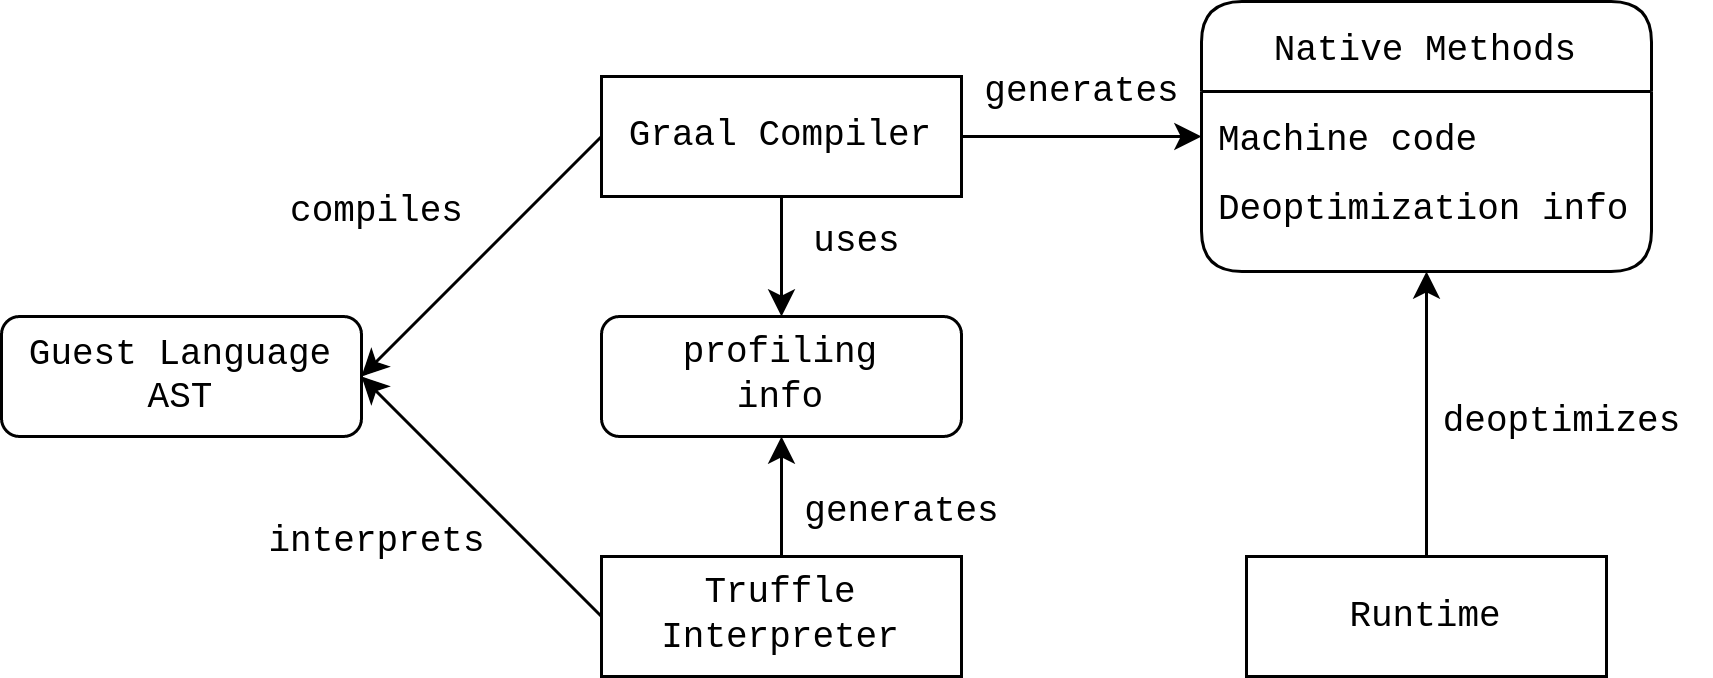
\includegraphics[width=0.5\textwidth]{figures/graalvm-pipeline.png}
	\caption{GraalVM overview\cite{graalvm:ir}.}
	\label{figure:graalvm-overview}
\end{figure}

Figure \ref{figure:graalvm-overview} provides an overview on the interactions between the multiple components of GraalVM.
This thesis makes substantial use of both components of GraalVM to create a runtime for Scala programs using TASTy.
The runtime is able to incorporate source level information for speculative optimizations.

\subsection{Graal}

GraalVM incorporates an existing implementation of a JVM\cite{java:hotspot} for the actual execution of programs.
Graal is \textit{only} the general-purpose just-in-time compilation infrastructure tt optimizes the programs to be executed.
Graal is general-purpose in that it conducts analysis and optimization on the same intermediate representation, \textit{Graal IR}, regardless of the source language.
Notably, most implementations of a source language utilizing GraalVM have an implementation in Truffle.
In addition to a Truffle interpreter for Java bytecode\cite{graalvm:espresso}, there is a direct translator for Java programs in GraalVM that parses Java bytecode into Graal IR.

Graal IR\cite{graalvm:ir} is an IR suitable for speculative optimizations, while still retaining information from the Truffle guest language AST.
Graal IR is based on the \textit{sea of nodes} concept\cite{click:sea-of-nodes} and satisfies the \textit{static single-assignment}\cite{ssa} property.
A sea of nodes is an abstraction based on a directed graph structure that relates the control-flow graph\cite{allen:ctrl-flow-analysis} of a program to its data-flow graph\cite{allen:data-flow-analysis}.
An intermediate representation is in single-static assignment form when each variable is defined before it is used.\cite{johnson:use-def-chains}.

GraalIR enables Graal to speculatively compile only the \textit{hot} branches\cite{graalvm:speculative-ir}, or branches that are most frequently taken in the control flow portion of the IR, and their transitive data dependencies.
When a compiled program violates any underlying assumptions, execution is \textit{deoptimized}\cite{self:deoptimization} and the program resumes execution in the interpreter.
Deoptimization occurs when the compiled program is no longer considered stable and valid.
Graal automatically inserts \textit{guard nodes} into the IR, which are conditional checks validating if speculative assumptions used to compile the program still hold.
Deoptimization is part of an execution loop between Graal and Truffle, which allows GraalVM to adapt aggressively and speculate to find the best optimization in a dynamic execution environment.

\subsection{Truffle}

\begin{figure}[!htb]
	\centering
	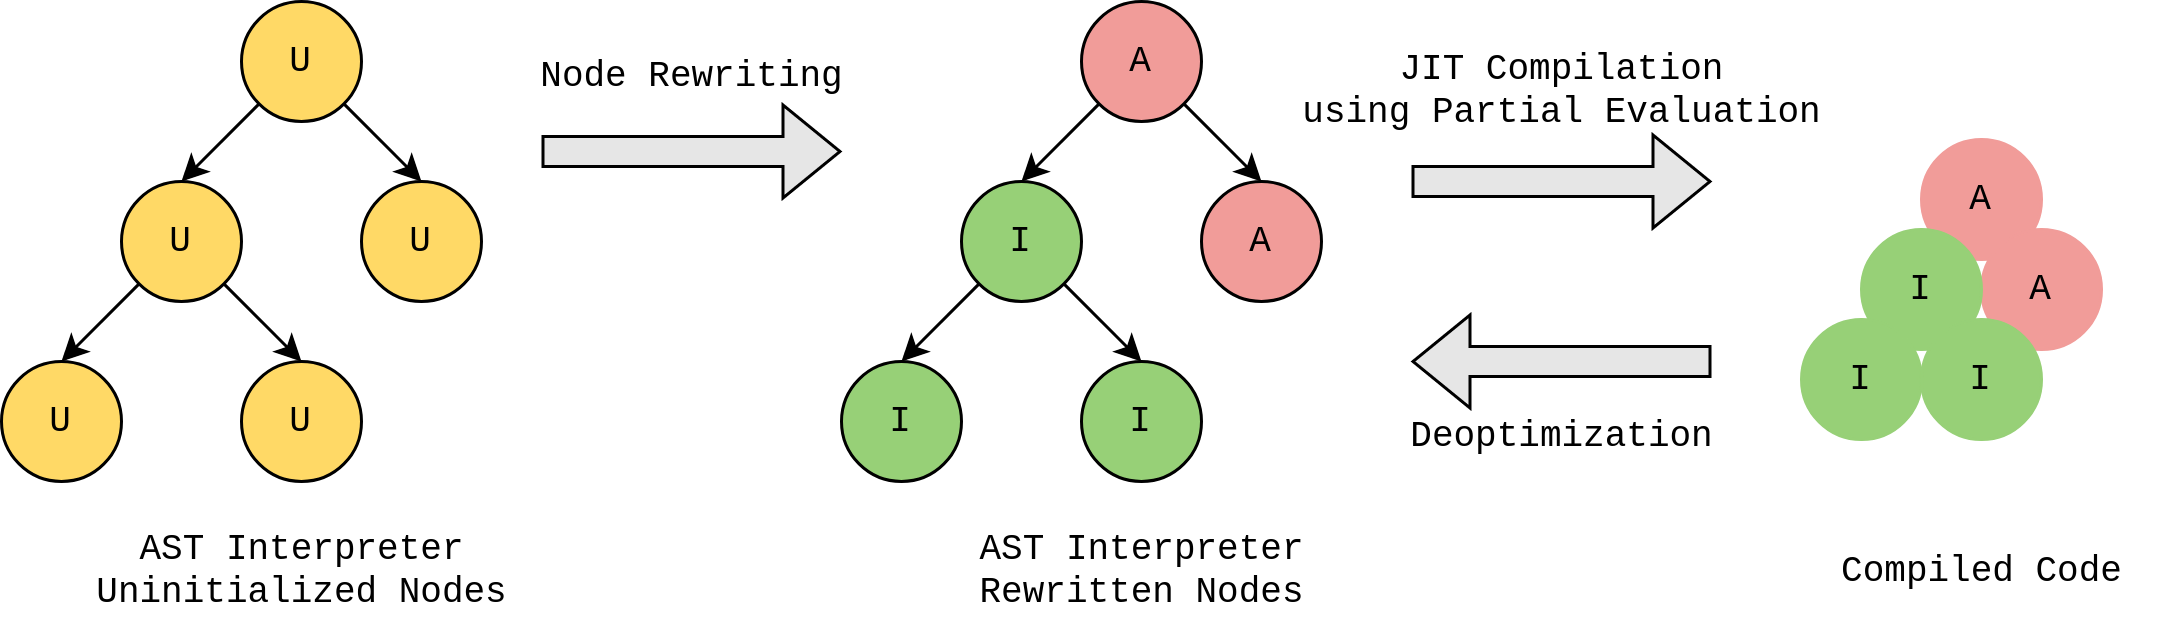
\includegraphics[width=0.75\textwidth]{figures/truffle-loop.png}
	\caption{Truffle's approach to self-optimization\cite{truffle:thesis}.}
	\label{diagram:graal-loop}
\end{figure}

Truffle is a framework for implementing an interpreter embedded into GraalVM.
Truffle differs significantly from other implementations of interpreters.
Interpreters can usually be divided into two subsets: tree interpreters and bytecode interpreters.
Tree interpreters transform the program source into an AST. 
AST interpretation has the added benefit of executing an intermediate representation close to the program source representation and is, therefore, more amenable to program optimization.
In contrast, bytecode interpreters, such as the JVM, execute a vastly simplified representation of programs.
While interpreters of bytecode programs tend to be faster than their tree counterparts, the absence of detailed source information, such as types, often makes program optimization difficult.
The problem of efficiently executing bytecode while retaining the ability to optimize them effectively using source program information is difficult for Scala on the JVM. 

Truffle is an atypical tree interpreter in that it combines the definition, execution, and optimization of an AST structure into a single abstraction.
While the structure of input programs in other interpreters is independent of the implementation of the interpreter, a Truffle interpreter is integrated into the structure of its input.
More concretely, this means an implementation of a Truffle interpreter is a collection of subclasses that extend \javainline{Node} class and implement a \javainline{execute()} method.
An interpreter is derived from implementing its input tree structure by defining execution semantics inside the AST to be executed.

During the execution of the AST, profiling information collected from the interpreter is used to drive \textit{node rewriting} and just-in-time compilation.
While Graal is language-agnostic, Truffle is able to exploit guest-language semantics for dynamic optimizations.
This process of replacing nodes in the AST with better, specialized guest-language counterparts in Truffle is called node rewriting.
Node rewriting makes Truffle abstract syntax trees self-optimizing and serves two purposes.
The first is to incorporate guestlanguage semantics into the executing program dynamically.
The second is to augment the AST for more efficient JIT compilation.
The nature of compiler optimizations requires that programs are incrementally simplified in order to be optimized.
While such types of optimizations are widely applicable to many languages using the JVM, node rewriting is a high-level language-specific optimization that occurs \textit{before} such simplifications.

The self-optimizing execution semantics of the AST are implemented with the Truffle \acrfull{dsl}.
The Truffle DSL is a mechanism to allow a \textit{guest language} to integrate semantics into a Truffle AST for self-optimization.
A guest language is a set of semantics, most commonly a programming language, encoded into a Truffle AST.
In this thesis, the guest language that our Truffle AST encodes and executes is TASTy (which represents Scala).

\begin{figure}[!htb]
\begin{minted}{scala}
abstract class EqualsNode extends BinaryOpNode {
	@Specialization
	def equalsInt(lhs: Int, rhs: Int): Boolean = lhs == rhs
	
	@Specialization
	def equals(lhs: Any, rhs: Any): Boolean = {
		if (lhs == null) 
		rhs == null 
		else 
		lhs.equals(rhs)
	}
}
\end{minted}
\caption{Pseudocode for a Truffle node implementation of an equality which supports node rewriting.}
\label{example:node-rewriting}
\end{figure}

Figure \ref{example:node-rewriting} demonstrates an example of the node that supports rewriting declared using the Truffle DSL.
The node declares semantics of the equality operation between integers and values of type \scalainline{Any}.
This equality node has semantics for every type because the \scalainline{Any} type is the supertype of all types in Scala.
A Truffle node that supports node rewriting begins in an uninitialized state.
When both the left and right-hand side operands are integers, the node is rewritten to \javainline{equalsInt} state.
When arguments of any other combination of types are detected, either in the uninitialized state or the \javainline{equalsInt} state, the node is rewritten to the \javainline{equals} state.


\begin{figure}[!htb]
\begin{minted}{java}
@GeneratedBy(EqualsNode.class)
public final class EqualsNodeGen extends EqualsNode {
	@Child private TermNode lhs_;
	@Child private TermNode rhs_;
	@CompilationFinal private int current_state;
	
	private EqualsNodeGen(TermNode lhs, TermNode rhs) {
		this.lhs_ = lhs;
		this.rhs_ = rhs;
	}
	
	public Object execute(VirtualFrame frame) {
		return (current_state & 2) != 0 && current_state != 0 ? 
			this.execute_int_int0(state, frame) : 
			this.execute_generic1(state, frame);
	}
	
	private Object execute_generic1(int state, VirtualFrame frame) {
		Object lhs = this.lhs_.execute(frame);
		Object rhs = this.rhs_.execute(frame);
		if ((state & 1) != 0 && lhs instanceof Integer) 
			if (rhs instanceof Integer) 
				return this.executeInt((Integer) lhs, (Integer) rhs);
		
		if ((state & 2) != 0) return this.executeObject(lhs, rhs);
		
		CompilerDirectives.transferToInterpreterAndInvalidate();
		return this.executeAndSpecialize(lhs, rhs);

	}	
}
\end{minted}
\caption{Generated code by the Truffle DSL for the \scalainline{AnyEqNode}.}
\label{impl:node-rewriting-gen}
\end{figure}

Figure \ref{impl:node-rewriting-gen} gives the auto-generated Java program that implements the semantics defined in \ref{example:node-rewriting}.
We will not discuss the semantics of every possible state in our generated node for brevity.
Instead, we will discuss the possible state transitions when a node starts in the uninitialized state.
State transitions are encoded as methods that execute the semantics for a given state, and update said state.
States are encoded as bit fields.
The uninitialized state is the $0$ value with no states encoded.
The \scalainline{equalsInt} state is encoded with $1$ and the \scalainline{equals} state is encoded with $2$.
\javainline{execute_generic1} is invoked when no states (specializations) are active in a \scalainline{EqualsNode}.
The first state transition checks whether the node is in one of two possible states (\scalainline{equalsInt} or \scalainline{equals}).
The corresponding specialization is invoked if the node is in either state and its arguments satisfy the preconditions.
This portion of the node may exist in either interpreted or compiled code.
However, if the node is not initialized, i.e., it is in neither possible state, the code is deoptimized (if compiled), and execution resumes from the interpreter.
While we do not showcase this, it is possible for a node to be in multiple states during execution.

The \javainline{executeAndSpecialize} method (figure \ref{impl:node-rewriting-specialize}) initializes the node to a specialized state.
If both arguments satisfy the \javainline{Int} type check invariant, the node is initialized to the \scalainline{equalsInt} state.
Otherwise, it is initialized to the \scalainline{equals} state.
Subsequent executions of the newly initialized node will invoke the appropriate specialization as long as their respective invariants are maintained.
Node rewriting narrows down a node's best implementation(s) for a particular profile of values.
If a Truffle AST cannot be rewritten further, it is considered \textit{stable}.
Stable nodes vastly simplify JIT compilation because of partial evaluation, a critical transformation applied to ASTs for JIT compilation that we will describe next.

\begin{figure}[!htb]
\begin{minted}{java}
private boolean executeAndSpecialize(Object lhs, Object rhs) {
	int prev_state = this.state_0_;
	if (lhs instanceof Integer) 
		if (rhs instanceof Integer) {
			this.current_state = prev_state |= 1;
			return this.equalsInt((Integer) lhs, (Integer) rhs);
		}

	this.current_state = prev_state |= 2;
	return this.equals(lhs, rhs);
}
\end{minted}
\caption{Implementation of \scalainline{executeAndSpecialize} of \scalainline{EqualsNodeGen}}
\label{impl:node-rewriting-specialize}
\end{figure}


When invocations of a root node exceed a predefined upper bound, Graal JIT compiles its children trees into native machine code using \textit{partial evaluation}.
Partial evaluation is a program optimization technique for specializing a program (code) for a given input (data)\cite{futamura:partial-eval}.
In the context of Truffle, this means specializing an AST node (code) based on the values, or types of values produced by their children nodes (data)\cite{truffle:partial-eval}.
The specialization of an AST node may also be based of the types of children nodes themselves.
We can say that the partial evaluation of an AST  will produce an AST that is \textit{specialized} for a particular set of values, or more commonly, in our case, a particular set of types.

For example, consider the partial evaluation of an \scalainline{EqualsNodeGen} node in the \scalainline{equalsInt} state.
The \javainline{current_state} field of the node is annotated with the \javainline{CompilationFinal} directive.
Truffle provides the \javainline{CompilationFinal} directive to indicate that a non-constant value in the guest-language implementation \textit{will} be a constant when being partially evaluated.
Because the state is a compilation constant, the condition on line $17$ of figure \ref{impl:node-rewriting-gen} evaluates to \javainline{true} when the state is $1$ (\scalainline{equalsInt}).
As a result, only the code for \javainline{execute_int_int0} (provided in \ref{impl:node-rewriting-state2}) will be compiled.
The generated implementation of \javainline{execute_int_int0} contains checks for the specialization invariant.
These checks act as points in the control flow of the compiled code to deoptimize, if these invariants are violated.
The resulting code supplied to the JIT compilation is the specialization of the \scalainline{EqualsNode} for the \scalainline{equalsInt} state.

\begin{figure}[!htb]
\begin{minted}{java}
private Object execute_int_int0(int state, VirtualFrame frame) {
	int lhs_int;
	try {
		lhs_int = this.lhs_.executeInt(frame);
	} catch (UnexpectedResultException ex) {
		Object rhs = this.rhs_.execute(frame);
		return this.executeAndSpecialize(ex.getResult(), rhs);
	}
	
	int rhs_int;
	try {
		rhs_int = this.rhs_.executeInt(frame);
	} catch (UnexpectedResultException ex) {
		return this.executeAndSpecialize(lhs_int, ex.getResult());
	}
	
	assert (state & 1) != 0;
	return this.executeInt(lhs_int, rhs_int);
}
\end{minted}
\caption{Implementation of \scalainline{execute_int_int0} of \scalainline{EqualsNodeGen}}
\label{impl:node-rewriting-state2}
\end{figure}

The sequence of optimizations given in figure \ref{diagram:graal-loop}, node rewriting, partial evaluation, and deoptimization is the advantage that a TASTy Truffle interpreter has over the traditional JVM bytecode interpreter for Scala.
Truffle allows for the incorporation of source-level type information into the just-in-time compilation loop.
This thesis will focus on using these features to execute TASTy with type information to augment JIT compilation.


%======================================================================
\chapter{The Monomorphic Interpreter}
\label{chapter:implementation}
% \epigraph{Typing is no substitute for thinking.}{Dartmouth Basic manual, 1964}

This chapter will describe the methods used to transform TASTy to make it suitable for a Truffle interpreter, \textsc{TastyTruffle}, \textit{without} polymorphism.
In particular, it will cover how to translate the organization of data and code in the \scalainline{DefDef}, \scalainline{ClassDef}, and \scalainline{Term} tree nodes into a Truffle implementation, which is amenable to execution and JIT optimization.
Chapter \ref{implementation:specialization} will then discuss extensions to our implementation to support parametric polymorphism and cover the techniques we use to specialize nodes to eliminate autoboxing in the presence of polymorphism. 

Scala programs in \acrshort{tasty} format are unsuitable for execution in a Truffle interpreter. 
Programs in TASTy must be parsed and transformed into an executable representation in Truffle.
These transformations translate the TASTy tree structure into a more straightforward but semantically equivalent Truffle AST.
For the rest of this thesis, we refer to the Truffle AST of TASTy as \textit{TastyTruffle IR}.
As TASTy represents a Scala program close to its equivalent source representation, canonicalization compiler passes (see appendix \ref{appendix:dotty-phases}) that would otherwise normalize the IR are not present. 
Instead, we implement TastyTruffle IR to represent a canonicalized executable intermediate representation that can later be specialized on demand. 

\begin{figure}[!htb]
	\begin{minted}{scala}
	def parseTopLevel(tree: Tree): Object = tree match {
		case vdef: ValDef   => 
			lazy val obj = initializeObject(vdef)
			registerObject(vdef.symbol, obj)			
		case cdef: ClassDef => 
			registerShape(cdef.tpe, parseClassDef(cdef))	
		case _ => ()
	}
	\end{minted}
	\caption{Pseudocode to evaluate every top level tree.}
	\label{impl:top-level}
\end{figure}

Figure \ref{impl:top-level} gives an evaluation loop typical in other interpreters in the context of this one.
A top-level tree is any tree without a parent.
In our subset of TASTy, a top level tree may be a \scalainline{ValDef} (a singleton object) or a \scalainline{ClassDef}.
Here we only present the pseudocode sufficient to traverse a program in TASTy. 
Each top-level definition is parsed and saved in a global interpreter context (\scalainline{registerShape} and \scalainline{registerObject}).
Top-level objects are lazily initialized as their class definitions may not have been parsed.
Registered objects and classes are then used in subsequent executions of the program.

We omit details on \textit{how} to execute the program to be concise.
Entry points in \scalainline{TASTy} are defined by a special method \scalainline{main}.
As multiple entry points may exist in a given program, we consider the selection of entry points as an implementation-specific detail.
In the following sections, we will describe the individual types of TASTy nodes, why some are directly unsuitable for execution, and how to simplify their semantics.

\section{Converting the \texttt{DefDef} tree into a Truffle \texttt{RootNode}}
\label{impl:subsection:defdef}

In this section, we describe the conversion of \scalainline{DefDef} trees to \textit{root nodes}.
\scalainline{DefDef} trees are the primary structure that organizes code (terms) in TASTY.
Root nodes represent the root of an executable Truffle AST, the primary abstraction that organizes code in Truffle.
In our case, root nodes are the Truffle analog of a \scalainline{DefDef}.
Each root node has a corresponding \textit{call target}, which is used for the invocation of the root node.
Call targets are the primary compilation unit for Graal.
A compilation unit is an organization of code that can be independently compiled.
A root node is automatically instrumented\cite{profiling:atom} to profile its number of invocations. 
When a root node has been frequently invoked inside the interpreter, it is JIT compiled into machine code by Graal.
Subsequent invocations of the call target will then use the more efficient compiled root node.

\begin{figure}[!htb]
\begin{minted}{scala}
abstract class RootNode(desc: FrameDescriptor) {
	def execute(frame: VirtualFrame): Object
	def getCallTarget: CallTarget
}
\end{minted}
\caption{Pseudocode of a root node.}
\label{example:root-node}
\end{figure}

Figure \ref{example:root-node} gives a simplified implementation of a root node.
Each root node in Truffle has a \textit{frame descriptor} and execution semantics.
A guest language must subclass and implement its root node to enable function invocation semantics.

A frame descriptor describes guest language variables that are in scope during execution.
The abstract \javainline{execute} method describes the invocation behaviour of a root node.
When a root node is executed, it is always supplied with a \textit{frame}.
A frame contains the arguments supplied during invocation and storage slots for local variable definitions in the body of the method.

\begin{figure}[!htb]
\begin{minted}{scala}
class DefDef(
	_: String, 
	params: List[ParamClause], 
	_: TypeTree, 
	rhs: Option[Term]) extends Definition	
\end{minted}
\caption{Definition of a \texttt{DefDef} tree with names of less important members replaced with \texttt{\_}}
\label{recall:defdef}
\end{figure}

A further simplified definition of a \scalainline{DefDef} tree is provided in figure \ref{recall:defdef}.
This section focuses on two members of a \scalainline{DefDef} tree.
The parameters of a \scalainline{DefDef} tree are given by the \scalainline{params} field.
In practice, the type of a \scalainline{ParamClause} is an alias for the union type \scalainline{TypeParams {|} TermParams}, so we omit the \scalainline{ParamClause} definition.
A \scalainline{DefDef} tree will have a parameter section for type parameters when they are polymorphic and will always have a term parameters section.
\scalainline{DefDef} trees may optionally have a body defined in the \scalainline{rhs} field.
When trees do not have a body defined, they are abstract method definitions and do not have a corresponding root node in Truffle.
Only non-abstract method definitions with a body (a term) are executable.
The explanation f parsing of terms into nodes for execution is given in section \ref{impl:subsection:classdef}

\begin{figure}[!htb]
\begin{minted}{scala}
object FrameSlotKind extends Enumeration {
	type FrameSlotKind = Value
	val Object, Long, Int, Double, Float, Boolean, Byte = Value
}	
	
def getFrameSlotKind(tpe: Type): FrameSlotKind = 
	if (tpe.isPrimitive) 
		// Int => FrameSlotKind.Int
		// ...
		// Double => FrameSlotKind.Double
		getPrimitiveSlotKind(tpe)
	else  
		FrameSlotKind.Object
\end{minted}
\caption{Simplified implementation of \scalainline{FrameSlotKind}}
\label{impl:frameslot-kind}
\end{figure}

Each value definition in the parameters of a \scalainline{DefDef} will have a corresponding frame slot in its parent frame descriptor. 
A frame slot references a unique frame value in the context of a root node.
Truffle permits each frame slot in a frame descriptor to be described by a \textit{frame slot kind}.
In Truffle, there is a corresponding frame slot kind for reference types and each \acrshort{jvm} primitive type. 
The pseudocode of a frame slot kind and a method to convert a type into a slot kind is given in \ref{impl:frameslot-kind}.

Truffle profiles frame accesses to minimize the amount of autoboxing that occurs when reading from a frame slot with an \javainline{Object} kind. 
To eliminate unnecessary specialization of frame accesses where types are monomorphic and statically refer to a primitive type, a parameter is assigned the matching primitive frame slot kind in the frame descriptor. 
In cases where the type is not a primitive type or a polymorphic applied type, e.g. \scalainline{List[T]} but not \scalainline{T}, The \scalainline{Object} kind is assigned to the frame slot.
Otherwise, the type is a polymorphic parameter, which \textit{could} resolve to a primitive type, and the frame slot kind cannot be resolved statically.
We will defer discussion on handling parameters of such polymorphic types that cannot be resolved statically until section \ref{implementation:specialization}.

\begin{figure}[!htb]
\begin{minted}{scala}
case class LocalFrameVal(slot: FrameSlot, kind: FrameSlotKind)
	
class DefDefNode(
	desc: FrameDescriptor, 
	params: Array[LocalFrameVal], 
	body: TermNode) extends RootNode(desc) {
	override def execute(frame: VirtualFrame): Object = {
		copyArgumentsToFrame(frame)
		try {
			body.execute()
		} catch {
			case ex: ReturnException => ex.getValue
		}
	}	
		
	def copyArgumentsToFrame(frame: VirtualFrame): Unit = 
		for ((param, arg) <- params zip frame.getArguments) 
			param.kind match {
				case FrameSlotKind.Int =>
					frame.setInt(param.slot, arg.asInstanceOf[Int])
				...
				case FrameSlotKind.Double =>
					frame.setDouble(param.slot, arg.asInstanceOf[Double])	
				case _ =>
					frame.setObject(param.slot, arg)
			}
}
\end{minted}
\caption{Pseudocode for \scalainline{DefDefNode} and \scalainline{Parameter}}
\label{impl:defdefnode}
\end{figure}

Figure \ref{impl:defdefnode} provides the implementation of the \scalainline{DefDefNode} and its parameters, the root node equivalent of a \scalainline{DefDef}.
The execution of a \scalainline{DefDefNode} is divided into two stages, argument preparation, and execution.
First, the arguments of the frame constructed during invocation (see \ref{impl:subsection:apply}) are copied into their respective parameter frame slots.
Frames contain separate regions for values of each frame slot kind.
We copy each argument into the appropriate frame slot region based on the frame slot kind prescribed to a parameter.
Storing parameters in this manner eliminates any unnecessary boxing that would otherwise occur when passing primitives as arguments.

By default, all frames start off \textit{virtual}.
Virtual frames are Truffle abstractions that provide guest languages an opportunity to exploit escape analysis.
Escape analysis\cite{escape-analysis} reasons about the dynamic scope of object allocations. 
Truffle and Graal both exploit the observations of \textit{Partial Escape Analysis}\cite{java:partial-escape-analysis}, a path-sensitive variant of escape analysis, to enable the following optimizations for guest languages:

\begin{description}
	\item[Region Allocation\cite{java:escape-analysis,tofte:region-memory}] The substitution of heap allocations with stack allocations to eliminate unnecessary garbage collection.
	\item[Scalar Replacement\cite{java:escape-analysis-optimizations}] The complete elimination of an object allocation, where the fields of the replaced object are substituted by local variables.
\end{description}

\begin{figure}[!htb]
\begin{minted}{scala}
def parseDefDef(ddef: DefDef): DefDefNode = {
	val desc = new FrameDescriptor
	val parameters = self :: ddef.params.map {
		case vdef: ValDef => generateLocal(vdef, desc)
	}
		
	val body = parse(ddef.rhs)
	new DefDefNode(desc, parameters, body)
}
	
def generateLocal(vdef: ValDef, desc: FrameDescriptor): LocalFrameVal = {
	val kind = getFrameSlotKind(vdef.tpt.tpe)
	val slot = desc.addSlot(kind)
	Parameter(slot, kind)
}
\end{minted}
\caption{Pseudocode for parsing \scalainline{DefDef} into \scalainline{DefDefNode}}
\label{impl:parse-defdef}
\end{figure}

The virtual frame abstraction allows guest languages to read and write to a frame without the requirement to optimize their object allocations.
Instead, escape analysis and scalar replacement are responsible for optimizing guest language object allocations during partial evaluation. 
After arguments are copied into the frame, their values become available for access during the execution of the body.
The body of a \scalainline{DefDefNode} is then executed, and its computed value is returned.

Figure \ref{impl:parse-defdef} provides a summary on parsing a \scalainline{DefDef} tree into its Truffle equivalent \scalainline{DefDefNode}.
Frame slot and frame slot kinds provide an abstraction for parameters and arguments to be resolved before executing the main body in a \scalainline{DefDefNode}.
In addition to the parameters explicitly present in TASTY, the root node will have an additional parameter representing the method's receiver.
The receiver is an object instance whose class definition owns the method being invoked.
In Scala, every method invocation has a receiver.
In TASTy, this translates to every \scalainline{DefDef} is owned by a \scalainline{ClassDef}.
In the next section, we detail how to organize call targets in Truffle by using \scalainline{ClassDef} trees.

\section{Deriving a \texttt{Shape} from a \texttt{ClassDef}}
\label{impl:subsection:classdef}

A \scalainline{ClassDef} tree defines the layout of an object in TASTy.
The layout of an object dictates the values that an object instance stores and the methods that can be invoked on an object instance.
The data layout of an object in a Truffle interpreter is described by a \textit{shape}\cite{self:prototypes,truffle:object-model}.
A Shape is a language-agnostic model for defining the properties of an object instance in Truffle.
A property in a shape describes one member of an object instance; it has an identifier and a value.
A Truffle object instance consists of \textit{object storage}, which contains instance-specific data and its shape.
Shapes map property identifiers to object storage locations; guest languages interface with object storage indirectly through properties.
In this thesis, we use a \textit{static shape}, an immutable variant of a shape.
Normally, shapes are mutable, and their list of properties may change throughout the lifetime of a program\cite{truffleruby:object-model}.
However, programs that dynamically change the layout of their objects\cite{java:reflection} are beyond the scope of this thesis.

\begin{figure}[!htb]
\centering
\begin{minted}{scala}
class ClassDef(
	name:        String,
	constructor: DefDef, 
	parents:     List[Tree], 
	_:           Option[ValDef], 
	body:        List[Statement]
) extends Definition

class ClassShape(
	symbol:  Symbol,
	parents: Array[Symbol],
	fields:  Array[Field]
	methods: Map[MethodSignature, CallTarget]
	vtable:  Map[MethodSignature, Symbol]
) extends Shape
\end{minted}
\label{impl:classshape}
\caption{Pseudocode of \scalainline{ClassDef} and a shape for a \scalainline{ClassDef}.}
\end{figure}

Recall the definition of a \scalainline{ClassDef} in figure \ref{impl:classshape}.
Each \scalainline{ClassDef} tree can be transformed into a corresponding \scalainline{ClassShape}, given in figure \ref{impl:classshape}.
Figure \ref{impl:parse-classdef} provides a very simplified implementation of the steps to transform a \scalainline{ClassDef} into a \scalainline{ClassShape}.
The \scalainline{name} parameter of \scalainline{ClassDef} alone is insufficient to be used as an identifier for a \scalainline{ClassShape}.
Names do not disambiguate between classes of the same name declared in different packages.
Instead, we used the symbol of the \scalainline{ClassDef} tree as the identifier for the \scalainline{ClassShape}.
For the remainder of this thesis, we will use a \scalainline{ClassInstance} to refer to an object instance with properties described by a \scalainline{ClassShape}.

\begin{figure}[!htb]
\begin{minted}{scala}
def parseClassDef(cdef: ClassDef): ClassShape = {
	val parents = cdef.parents.map(_.symbol)
	
	val fields = cdef.body map {
		case vdef: ValDef => generateField(vdef)	
	}
	
	val methods = (cdef.constructor :: cdef.body) map {
		case ddef: DefDef => ddef.symbol.signature -> parseDefDef(ddef)
	}
	
	val vtable = cdef.symbol.methodMembers map {
		symbol => symbol.signature -> symbol
	}

	new ClassShape(cdef.symbol, parents, fields, init ++ methods, vtable)
}

def generateField(vdef: ValDef): Field = vdef match {
	case ValDef(_: String, tpt: TypeTree, rhs: Option[Term]) => 
		new Field(vdef.symbol, vdef.tpt.tpe)
}
\end{minted}
\caption{Pseudocode to convert a \scalainline{ClassDef} into a \scalainline{ClassShape}.}
\label{impl:parse-classdef}
\end{figure}

A \scalainline{ValDef} tree in the \scalainline{ClassDef} body translates to a field definition in the \scalainline{ClassShape}.
A \scalainline{ClassShape} has a collection of fields that implement the static shape property.
Figure \ref{impl:field} gives our implementation of a field.
Fields define operations to read and write from the object storage on a \scalainline{ClassInstance}.
Like frames with frame slot kinds, object instances in Truffle have separate regions for storing values of each primitive type and one for reference types.
Following the same rules with types and frame slot kinds described in section \ref{impl:subsection:defdef}, the data access of a field depends on the type of the \scalainline{ValDef} tree from which the field originates.
The remaining members of a \scalainline{ClassShape} do not describe data that has to be stored in the object storage of a \scalainline{ClassInstance}.

\begin{figure}[!htb]
\begin{minted}{scala}
class Field(symbol: Symbol, tpe: Type) extends StaticProperty {
	override def getId: String = symbol.name
	
	def get(instance: Object): Any = 
		if (tpe == Int) getInt(instance)
		else if ...
		else if (tpe == Double) getDouble(instance)
		else getObject(instance)
	
	def set(instance: Object, value: Any): Unit = 
		if (tpe == Int) setInt(instance, value.asInstanceOf[Int])
		else if ...
		else if (tpe == Double) setDouble(instance, value.asInstanceOf[Double])
		else setObject(instance, value)	
} 
\end{minted}
\caption{Pseudocode of the field property.}
\label{impl:field}
\end{figure}

After the constructor and the \scalainline{DefDef} statements of a \scalainline{ClassDef} are converted into root nodes, they are stored in the \scalainline{ClassShape} mapped by a method signature.
The pseudocode for a method signature is given in figure \ref{impl:method-signature}.
Method signatures disambiguate method invocations in the presence of \textit{overloading}\cite{strachey:fundamental-concepts}, where methods share the same name but have different arguments.
When combined with parametric polymorphism, method signatures must also be able to disambiguate between methods sharing the same name but having different type parameters.
However, method signatures do not have to disambiguate between different type parameters by name, only the number of type parameters a method has.
Because type erasure erases polymorphic type parameters from methods, generic methods that share the same number of type parameters, as well as the same parameter types, will conflict and therefore are invalid.
As previously mentioned, methods are shared among all \scalainline{ClassInstance} objects with the same shape; call targets are stored on their owning shape.

\begin{figure}[!htb]
\begin{minted}{scala}
case class MethodSignature(symbol: Symbol, params: Int, types: Array[Type])
\end{minted}
\caption{Pseudocode of a method signature.}
\label{impl:method-signature}
\end{figure}

Often a shape will not contain the call target referenced by a signature because the dispatch is dynamic, and the original type inherits the method.
A \scalainline{ClassShape} contains a \textit{virtual method table}, which maps a method signature to the symbol of a shape that contains the call target matching the signature.
If a method signature does not have a call target in the current shape, the shape which holds the target is indirectly resolved using the virtual method table during execution.
While this resolution carries significant performance overhead in Truffle and other programming language implementations, we will describe a technique that partially mitigates this overhead further in chapter \ref{implementation:specialization}.

\section{Transforming \texttt{Terms} into \texttt{Nodes}}

\begin{figure}[!htb]
\begin{minted}{scala}
abstract class TermNode extends Node with InstrumentableNode {

	def execute(frame: VirtualFrame): Object 
	def executeInt(frame: VirtualFrame): Int = execute(frame).asInstanceOf[Int]
	...
	def executeDouble(frame: VirtualFrame): Double = execute(frame).asInstanceOf[Double]

}
\end{minted}
\caption{Pseudocode of a TermNode.}
\label{impl:term-node}
\end{figure}

In this section, the conversion of \scalainline{Term} trees into Truffle nodes is given.
The Truffle \scalainline{Node} abstraction allows guest languages to implement executable fragments of an AST.
Figure \ref{impl:term-node} is our subclass of a Truffle \scalainline{Node}.
Subclasses of the \scalainline{TermNode} will define node-specific semantics encapsulating a particular functionality of the interpreter.
The \scalainline{TermNode} takes advantage of Truffle's autoboxing elimination by defining companion \scalainline{execute[TYPE]} methods to allow subclasses to declare when an expected result from a child node must conform to a specific primitive type.
In the following sections, we give the subclasses that individually implement the monomorphic interpreter's functionality.

\subsection{Creating Instances}

\begin{figure}[!htb]
\begin{minted}{scala}
def parseNew(new: New): NewNode = new NewNode(new.tpe.symbol)	

class NewNode(symbol: Symbol) extends TermNode {
	override def execute(frame: VirtualFrame): Object =  shapeOf(symbol.tpe).newInstance
}
\end{minted}
\caption{Pseudocode of a \scalainline{NewNode} and how it is parsed.}
\label{impl:new-node}
\end{figure}

The \scalainline{New} tree represents the allocation of an instance of a \scalainline{ClassDef}.
The Truffle equivalent allocate node given in figure \ref{impl:new-node} is not so different, but it allocates an instance with properties described by the \scalainline{ClassShape} instead of a \scalainline{ClassDef}.
Note that a \scalainline{NewNode} only \textit{creates} an object; the parameters and fields of an object remain uninitialized.
An object is \textit{initialized} when the type constructor, \scalainline{<init>}, is invoked on a newly created object.
TASTy is emitted with this sequence of events in mind; object creation is always followed by object construction.
Structurally, this means that a \scalainline{New} tree is always the child of an initializer \scalainline{Apply} tree.

\subsection{Function Application}
\label{impl:subsection:apply}

\begin{figure}[!htb]
\begin{minted}{scala}
def parseApply(apply: Apply): ApplyNode = {
	val signature = apply.symbol.signature
	apply match {
		case Apply(Select(qualfier, _), arguments) => 
			if (qualifier.tpe.isPrimitve)
				if (args.length == 0) unaryOp(signature, qualifier)
				else                  binaryOp(signature, qualifier, args(0))
			else if (qualifier.tpe.isArray)
				arrayOp(signature, qualifier, arguments)
			else 
				new ApplyNode(signature, parse(qualifier), arguments.map(parse))	
		}
	}
\end{minted}
\caption{Pseudocode of parsing an \scalainline{Apply} tree.}
\label{impl:parse-apply}
\end{figure}
The \scalainline{Apply} tree is a context-dependent tree that represents multiple types of operations.
The types of their receiver disambiguate these operations.
Figure \ref{impl:parse-apply} provides an overview of the transformations discussed in this section as pseudocode for parsing an \scalainline{Apply} into TastyTruffle IR.
We omit the implementations of \scalainline{unaryOp}, \scalainline{binaryOp}, \scalainline{arrayOp} to remain concise; 
These methods generate a Truffle intrinsic node, representing a similar JVM equivalent.
In the following sections, we enumerate all possible semantics in our subset of TASTy:

\subsubsection{Arithmetic and Logical Operators}

In TASTy, there are no unary and binary operators, typically found in Java or other imperative languages.
Unary and binary operators are an invocation of the 0-argument (unary operator) or 1-argument (binary operator) method. 
For example, the following addition operator in Scala \scalainline{1 + 2} is desugared to \scalainline{1.+(2)}. 
That is, the binary operator \scalainline{+} is represented as the invocation of the instance function \scalainline{Int.+} on the receiver with value \scalainline{1} and type \scalainline{Int} with a single argument \scalainline{2}.
Generally, in the Scala compilation pipeline, methods that operate on primitive types and have an equivalent bytecode instruction on the JVM\cite{java:vm-spec} are replaced by those instructions in compiled program bytecode. 
This process of selecting efficient implementations for numerical or logical operations is called intrinsification.
Similarly, TastyTruffle avoids implementing methods of primitive types with actual call semantics as primitive operations are frequently used and simplify optimization for Graal.

\subsubsection{Array Access}

The syntax for accessing array elements in Scala does not differ from the method invocation on an array.
In other imperative languages, such as Java, the syntax for accessing arrays is commonly separate from the syntax of invoking a method.
For example, the access \scalainline{array(0)} is desugared to \scalainline{array.apply(0)} once the program is emitted in TASTy.
However, an array write \scalainline{array(0) = 42} is desugared to \scalainline{array.update(0, 42)}.

Similar to unary and binary operators, the underlying implementation of array operations is intrinsified into JVM bytecode instructions where possible.
However, using the bytecode provided in figure \ref{example:contains-bytecode} as an analog, operations on polymorphic arrays \scalainline{cannot} be intrinsified.
Instead, polymorphic array operations are handled by functions in the Scala runtime library.
The overhead of such operations is substantial and commonly represents the most significant performance bottleneck in array-bound programs.
These costs are additionally abstracted from the user as they commonly arise when using array-backed collections from the Scala standard library.

To operate without specialization, the implementation of our interpreter also incorporates the same runtime code to handle polymorphic array operations.
The methods used to eliminate the runtime overhead of these polymorphic bridge methods will be covered in chapter \ref{implementation:specialization}.

\subsubsection{Method Invocation}

\begin{figure}[!htb]
\begin{minted}{scala}
@NodeChild("receiver")
@NodeField("signature", MethodSignature.class)
class ApplyNode(@Children args: Array[TermNode]) extends TermNode {
	final val INLINE_CACHE_SIZE: Int = 5;
	
	@Specialization(guards = "instance.getShape == shape", limit = "INLINE_CACHE_SIZE")
	def cached(
		frame: VirtualFrame,
		instance: ClassInstance,
		@Cached("instance.getShape") shape: ClassShape,
		@Cached("create(resolveCall(instance, signature)") callNode: DirectCallNode
	): Object = callNode.call(evalArgs(frame, instance));
	
	@Specialization(replaces = "cached")
	def virtual(
		frame: VirtualFrame,
		instance: ClassInstance,
		@Cached callNode: IndirectCallNode
	): Object = {
		val callTarget = resolveCall(instance.getShape, signature);
		callNode.call(callTarget, evalArgs(frame, instance))
	}
}
\end{minted}
\caption{Simplified implementation of the call node with a polymorphic inline cache used in TastyTruffle.}
\label{implementation:poly-cache-call-node}
\end{figure}

Otherwise, the \scalainline{Apply} tree encodes a `normal' method invocation.
Truffle provides two abstractions for call nodes.
The \textit{direct call node} is used when the call target can be statically resolved. 
In our subset of TASTy, this is the set of methods with private or final modifiers\cite{java:lang-spec} and class constructors. 
Otherwise, the Truffle \textit{indirect call node} is used for calls where call targets must be dynamically resolved. 
Using indirect calls instead of direct calls comes with a performance overhead as indirect call nodes are difficult to inline and inhibit Graal's dynamic intraprocedural analyses.
In this thesis, we describe a call node implementation for both statically and dynamically dispatched calls. 
In order to minimize the use of indirect call nodes, we take advantage of a polymorphic inline cache\cite{self:polymorphic-inline-caches} to eliminate the overhead of resolving virtual calls for \acrshort{jit} compilation. 

Figure \ref{implementation:poly-cache-call-node} shows a simplified Truffle call node in \textsc{TastyTruffle} that implements a polymorphic inline cache.
The \scalainline{ApplyNode} is declared using the Truffle DSL.
The \scalainline{@NodeChild} and \scalainline{@NodeField} annotations declare that the DSL should generate children and properties of those names and types, respectively. 
The \scalainline{@Specialization} annotation declares the node writing semantics for method invocation.
Because we have defined a limit on the number of specializations, the DSL will also generate additional code for a polymorphic inline cache.
This cache saves call targets based on the type of receiver seen at the call site. 

When the type of receiver has not been seen in the inline cache, an additional cache entry is generated and appended to the cache for the next call.
Because a polymorphic inline cache dispatches direct calls based on the type of the receiver value seen, Graal can speculatively optimize the call site with the assumption that the receiver is always the same type and, therefore, the call target does not change among invocations.
Furthermore, this allows the calls site to be inlined, allowing a feedback loop of intraprocedural optimizations\cite{conditional-constant-prop,variable-congruence} to propagate through the inlined tree.
One important aspect to note is that the size of a polymorphic inline cache must be kept reasonable such that the cost of searching the cache does not defeat the speedup afforded by using the cache.
If the size of the cache exceeds an implementation-specific limit, the caller node is rewritten to use an indirect call.
The cache size is often decided based on profiling and heuristics to balance the cost of inline cache lookup against the penalty of an indirect call. 

\begin{figure}[!htb]
	\centering
	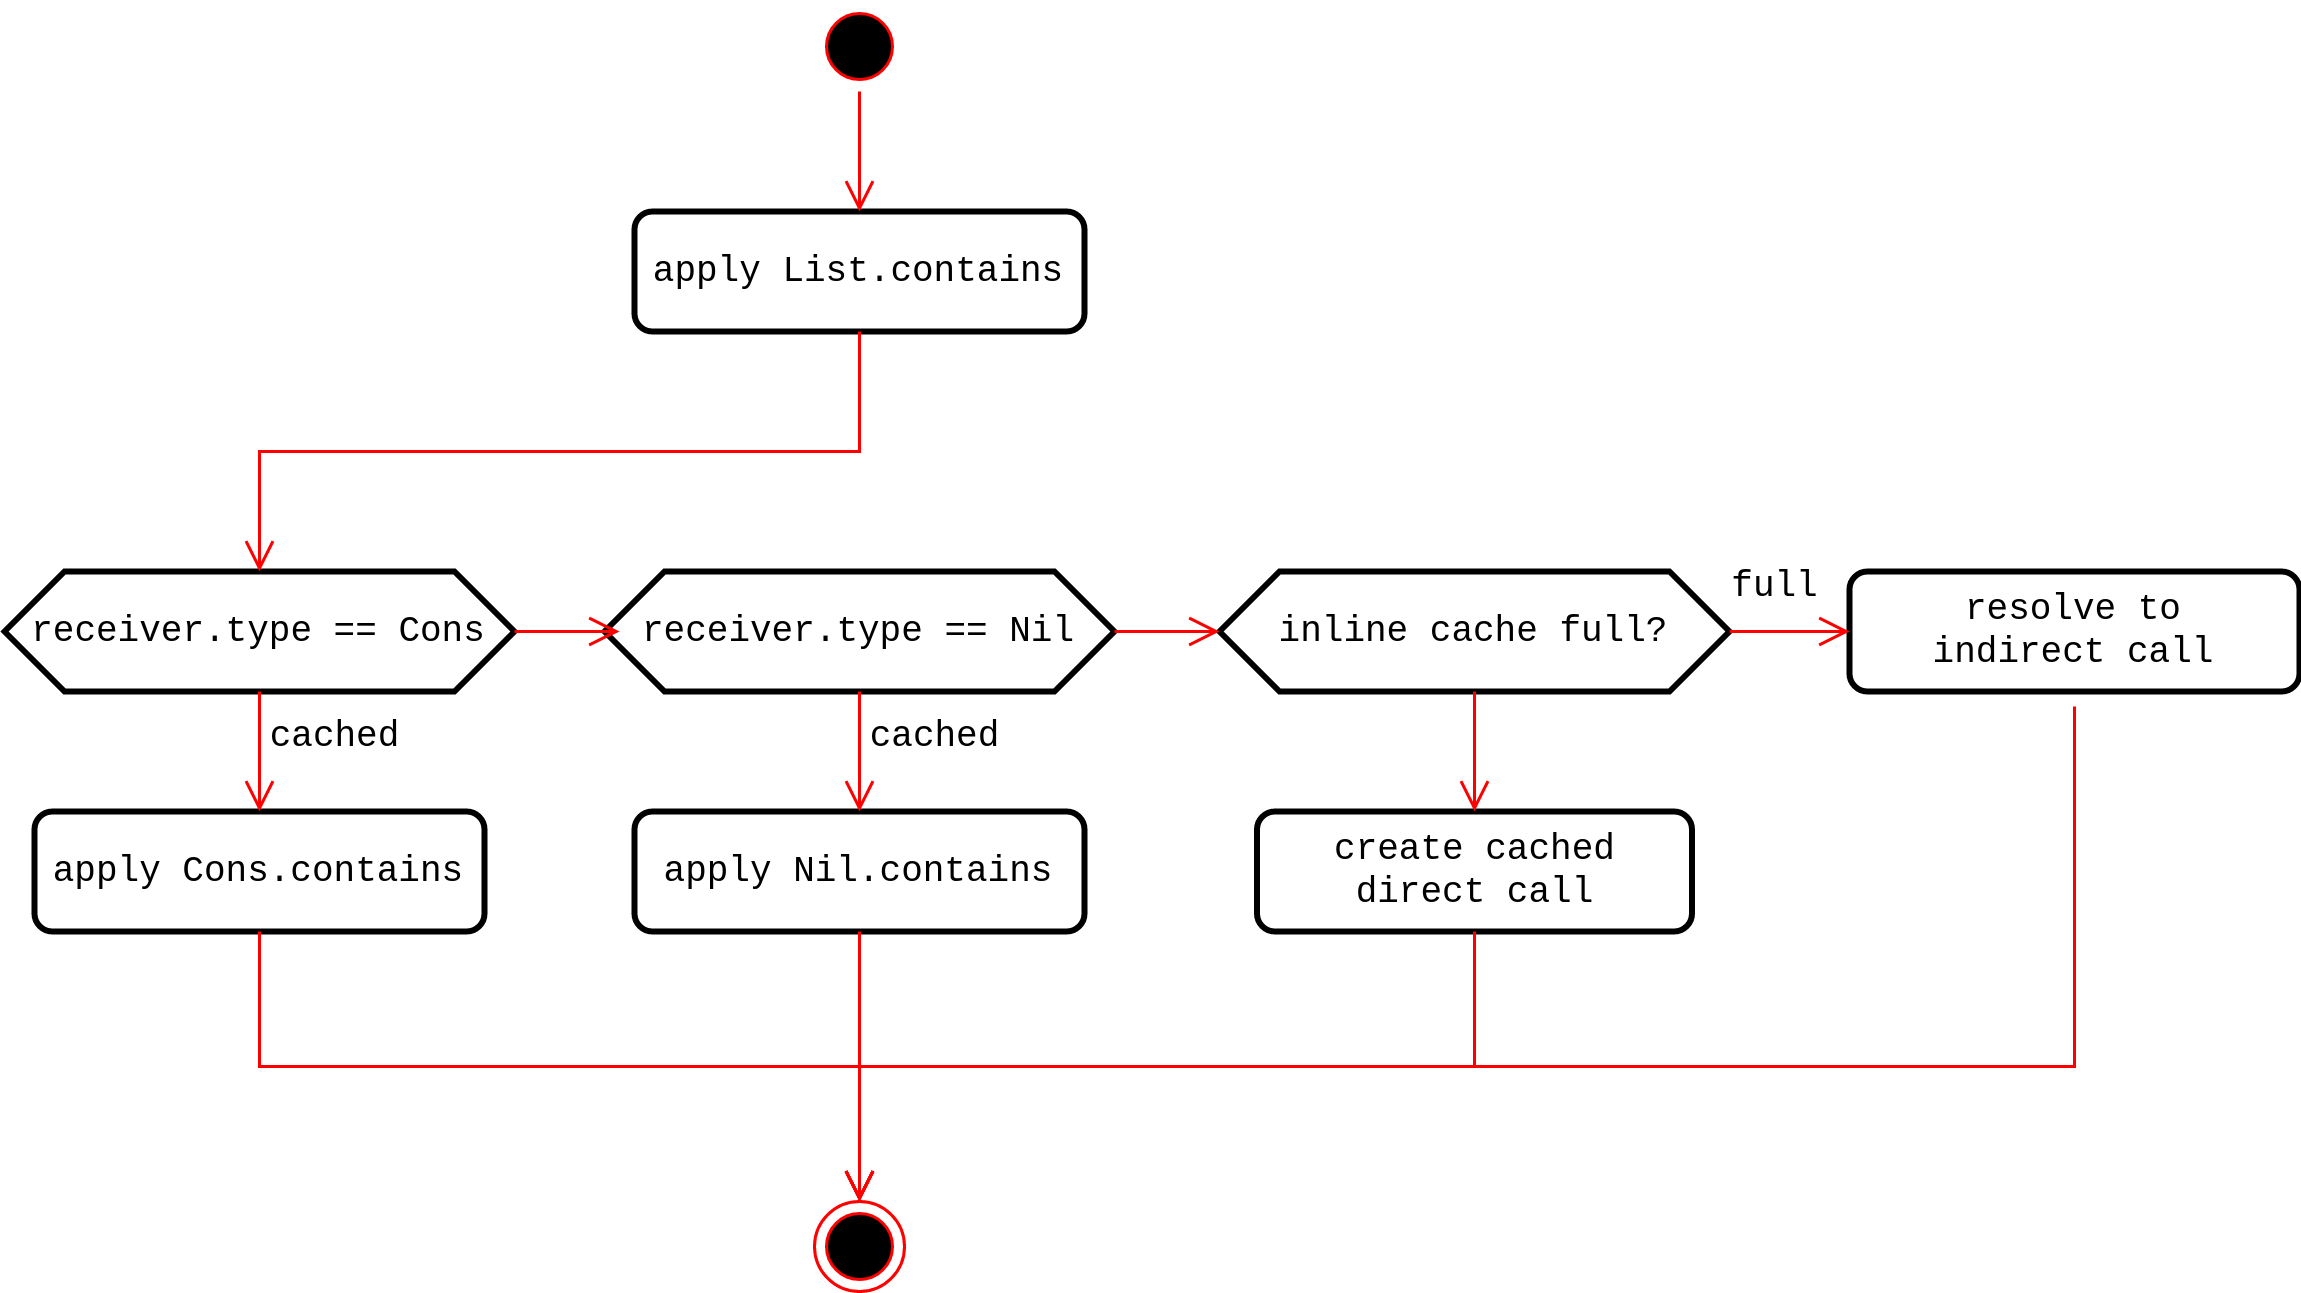
\includegraphics[width=0.6\textwidth]{figures/tastytruffle-pic-example.png}
	\caption{A possible polymorphic inline cache for a \scalainline{List.contains} callsite.}
	\label{example:poly-cache-call-node}
\end{figure}

Figure \ref{example:poly-cache-call-node} shows a data flow diagram of the application of a polymorphic inline cache to a call site of \scalainline{contains} when the receiver type is statically known to be \scalainline{List}. 
The diagram shows that the call site was previously called with a receiver where the dynamic type has been both \scalainline{Cons} and \scalainline{Nil}.
The \scalainline{ApplyNode} will first check if the type of receiver at the call site has the type \scalainline{Cons}; If the check passes, then the cached direct call node is invoked, and the call is complete.
It will do the same for the type \scalainline{Nil}.
Otherwise, the type of receiver has not been seen before, and the call target is resolved virtually and then cached for the following invocation at this call site.

When the polymorphic inline cache is applied to a monomorphic call site (where the type of the receiver does not change), it simplifies to a single element inline cache\cite{smalltalk:inline-caches}. 
Because the type of the receiver at the call site remains stable, the cache look-up of the call target based on the type always succeeds, and the call site never fall backs to using an indirect call node.

\subsection{Accessing Fields}

In our subset of TASTy, the \scalainline{Select} tree represents a read of a field of a \scalainline{ClassInstance}.
Notice in the resolution of the \scalainline{Apply} tree that the \scalainline{Apply} tree represents a method invocation, when the applicator is a \scalainline{Select}.
Because functions are first-class objects in Scala, the TASTy tree for a method invocation is the access of a method as if it were a field, then the application of result to a list of arguments.
Since this case has been previously handled when parsing the \scalainline{Apply} tree, a \scalainline{Select} tree always selects a value definition.

\begin{figure}[!htb]
\begin{minted}{scala}
@NodeChild("receiver")
@NodeField("symbol", Symbol.class)
abstract class ReadFieldNode extends TermNode {
	final val INLINE_CACHE_SIZE: Int = 3;
		
	@Specialization(guards = "instance.getShape == shape", limit = "INLINE_CACHE_SIZE")
	def cached(
		instance: ClassInstance,
		@Cached("instance.getShape") shape: ClassShape,
		@Cached("lookupField(shape)") field: Field
	): Object = field.getContents(instance)
		
	@Specialization(replaces = "cached")
	def virtual(instance: ClassInstance): Object = {
		val field = lookupField(instance.getShape)
		field.getContents(instance)
	}

	private def lookupField(shape: ClassShape): Field = shape.getField(symbol)
}
\end{minted}
\caption{Pseudocode of field read node with a polymorphic inline cache.}
\label{impl:field-read-node}
\end{figure}

However, fields may only be directly accessed in the immediate class scope.
Field access from an outside context is achieved through an \scalainline{accessor}.
Accessors are special methods generated in the compilation pipeline solely to access a field because the Scala compiler enforces the \textit{uniform access principle}\cite{beyer:oo-construction} for all programs.
We apply the transformation to generate accessors in class definitions because accessors are normally generated after TASTy is emitted in the standard Scala compilation pipeline.
Accessors also conveniently provide a mechanism to resolve indirect field access.
Indirect field access occurs when an inherited field is accessed in a subclass.
As we already have a mechanism for resolving method applications, we will combine this mechanism with a new direct field read node to implement field access.

Figure \ref{impl:field-read-node} gives a simplified implementation of a field read node.
Like the virtual dispatch of call targets, fields are resolved dynamically with the shape of a \scalainline{ClassInstance}.
We apply a polymorphic inline cache to the lookup of field properties to eliminate the performance overhead associated with this kind of virtual dispatch.

\subsection{Accessing Locals and Globals}

\begin{figure}[!htb]
\begin{minted}{scala}
def parse(ident: Ident): TermNode = {
	if (ident.symbol.isObjectDef)
		new ReadGlobalNode(symbol)
	else 
		new ReadLocalNode(localOf(symbol))
}
\end{minted}
\caption{Pseudocode to parse an \scalainline{Ident} tree.}
\label{impl:parse-ident}
\end{figure}

The \scalainline{Ident} tree is a name that refers to either a local or global value.
Local values take the form of a local variable or a method parameter.
Global values refer to top-level \scalainline{object} definitions.
We differentiate between a local and a global based on whether the symbol of the \scalainline{Ident} tree refers to a singleton top-level \scalainline{object} definition (shown in figure \ref{impl:parse-ident}).

\begin{figure}[!htb]
\begin{minted}{scala}
object Globals {
	val values: Map[Symbol, ClassInstance]
}

class ReadGlobalNode(symbol: Symbol) extends TermNode {
	override def execute(frame: VirtualFrame): Object = Globals.values.get(symbol)
}

class ReadLocalNode(local: Local) extends TermNode {
	override def execute(frame: VirtualFrame): Object = frame.getObject(local.index)
}
\end{minted}
\caption{Pseudocode of local and global value read nodes.}
\label{impl:local-global-node}
\end{figure}

Figure \ref{impl:local-global-node} provides the pseudocode implementations of \scalainline{ReadGlobalNode} and \scalainline{ReadLocalNode}.
In our interpreter, local variables and method parameters are uniformly represented by the frame slot abstraction.
During parsing, it is sufficient to maintain a mapping from symbols to a \scalainline{Local} to resolve which local variable is read.
Truffle does not provide an abstraction for storing global values.
Instead, we retain a mapping of symbols to instances for all global object value definitions.
Recall from figure \ref{impl:top-level} that a top-level value definition is registered.
When the symbol of an \scalainline{Ident} refers to a \scalainline{ObjectDef}, or a top-level \scalainline{ValDef}, it is resolved using the symbol to look up top-level global values previously registered in \ref{impl:top-level}.

\subsection{Mutating Values}

\begin{figure}[!htb]
\begin{minted}{scala}
def parseAssign(assign: Assign): TermNode = assign match {
	case Assign(select: Select, rhs) => 
		new WriteFieldNode(parse(select.qualifier), select.symbol, parse(rhs)) 
	case Assign(ident: Ident, rhs) =>
		new WriteLocalNode(localOf(ident.symbol), parse(rhs)) 
}
\end{minted}
\caption{Pseudocode to parse an \scalainline{Assign} tree.}
\label{impl:parse-assign}
\end{figure}

The \scalainline{Assign} tree has context-dependent semantics based on the structure of its left-hand side term.
Figure \ref{impl:parse-assign} contains the simplified logic to resolve \scalainline{Assign} trees into the appropriate term nodes.
If the left-hand side term is a \scalainline{Select} tree, the current tree mutates the field of a \scalainline{ClassInstance}.
Otherwise, the left-hand side is an \scalainline{Ident} which refers to the local variable in the frame.
We differentiate between which node to generate based on the type of the tree seen on the left-hand side.
\scalainline{WriteFieldNode} and \scalainline{WriteLocalNode} mirror their read node counterparts, but instead of reading from their respective locations, they update the value at their locations.
Like field reads, field writes in scopes outside of the class are dispatched through \textit{mutators}.
Mutators serve the same purpose as accessors but carry an argument to update the value of the field.

\subsection{Conditionals}

\begin{figure}[!htb]
\begin{minted}{scala}
def parseIf(i: If): IfNode = {
	new IfNode(parse(i.cond), parse(i.thenp), parse(i.elsep))
}
	
class IfNode(
	@Child cond: TermNode, 
	@Child t: TermNode, 
	@Child f: TermNode) extends TermNode {
	val cp = ConditionProfile.create();
		
	override def execute(frame: VirtualFrame): Object =
		if (cp.profile(cond.executeBoolean(frame)))
			t.execute(frame)
		else 
			f.execute(frame)		
}
\end{minted}
\caption{Pseudocode for parsing an \scalainline{If} into an \scalainline{IfNode}}
\label{impl:if}
\end{figure}

The implementation of conditional control flow in our interpreter is quite simple.
Two execution paths exist for the two possible results from evaluating the condition term; the path taken depends on the boolean after evaluation.
An \scalainline{IfNode} is derived from an \scalainline{If} tree (given in figure \ref{impl:if}), which allows for divergence in program control flow.
The implementation of the TastyTruffle IR mirrors the semantics given by its original TASTy tree.
In order to take advantage of conditional speculative optimization, we add a \javainline{ConditionProfile} onto the result of the condition term.
A condition profile records the likelihood that a branch is either true or false.
Graal then speculatively optimizes the frequently true or false branches of an \scalainline{IfNode} using its condition profile.

\subsection{Loops}

In our subset of TASTy, the \scalainline{While} tree is the only looping construct.
The control flow of the \scalainline{While} tree is quite simple; the body term is executed as long as the condition term holds at the beginning of every iteration.
Truffle provides the \scalainline{LoopNode} abstraction for implementations of guest language loop structures.
The loop node abstraction allows guest languages to take advantage of \textit{On-Stack Replacement}\cite{osr}.
On-stack replacement is a technique that switches control of part of a program running in the interpreter to compiled code while that part is executing.

\begin{figure}[!htb]
\begin{minted}{scala}
def parseWhile(tree: While): WhileNode = {
	new WhileNode(parse(tree.cond), parse(tree.body))	
}
	
class WhileNode(@Child cond: TermNode, @Child body: TermNode) extends TermNode {
	
	@Child val loopNode: LoopNode = 
		Truffle.getRuntime.createLoopNode(new WhileRepeatingNode(cond, body))
	
	override def execute(frame: VirtualFrame): Object = {
		loopNode.execute(frame)
		()
	}
	
	class WhileRepeatingNode(
		@Child cond: TermNode, 
		@Child body: TermNode
	) extends Node with RepeatingNode {
		val cp = ConditionProfile.create()
		
		override def executeRepeating(frame: VirtualFrame): Boolean = 
			if (cp.profile(cond.executeBoolean(frame))) {
				body.execute(frame)
				true 
			} else false 
			
	}
}
\end{minted}
\caption{Pseudocode for a \scalainline{WhileNode}}
\label{impl:while}
\end{figure}

So far in this thesis, the root node has been the primary compilation unit in Graal.
Root nodes profile their invocation count and get JIT compiled when they have been invoked frequently.
However, loop constructs that are executed for many iterations also justify JIT compilation.
The loop node is an additional type of JIT compilation unit which Graal can compile.
A key difference between loop nodes and root nodes is when their compiled equivalents are utilized.
While compiled root nodes are used in subsequent invocations of their call targets after they are JIT compiled, compiled loop nodes are used in the next iteration after they are JIT compiled.
As on-stack replacement is not a central focus of this thesis, we will only discuss it briefly, because loop nodes are the recommended abstraction for guest languages to implement loop structures in Truffle.

Figure \ref{impl:while} contains the implementation of a \scalainline{WhileNode} and its derivation from a \scalainline{While} tree.
Like our implementation of the \scalainline{IfNode}, we add a condition profile onto the node which evaluates the termination condition inside \scalainline{WhileRepeatingNode}.
Truffle will automatically instrument the \scalainline{WhileNode}.
After sufficient iterations of the \scalainline{WhileRepeatingNode}, the repeating node is compiled, and the next iteration of the \scalainline{WhileNode} will use the compiled repeating node.

\subsection{Blocks}

\begin{figure}[!htb]
\begin{minted}{scala}
def parseBlock(block: Block): BlockNode = {
	val desc = getParentFrameDescriptor(block)
		
	val terms = block.statements map {
		case vdef: ValDef => generateBlockLocal(desc, vdef)
		case term => term 
	}
		
	new BlockNode(terms, parse(block.expr))
}
	
def generateBlockLocal(desc: FrameDescriptor, vdef: ValDef): TermNode = {
	val local = generateLocal(vdef)
	new WriteLocalNode(local, parse(vdef.rhs))
}	
\end{minted}
\caption{Pseudocode for parsing \scalainline{Block} into \scalainline{BlockNode}}
\label{impl:parse-block}
\end{figure}

This section covers the translation of the \scalainline{Block} tree to its TastyTruffle IR equivalent.
The \scalainline{Block} is unique among term trees as it describes data and code.
In our subset of TASTy, this means that a block may contain declarations of local variables as well as executable terms.
Figure \ref{impl:parse-block} provides an overview on the transformations necessary to convert a \scalainline{Block} tree into \scalainline{BlockNode}.
We divide the discussion of blocks into the resolution of local variables when encountering a \scalainline{ValDef} tree and the execution of all other trees.

Local variables are bound to a \textit{scope}. 
A scope represents the lifetime in which a variable can refer to a value. 
Similarly, uses of variables are only valid when used under the appropriate scope. 
Local variables and their use sites are represented in intermediate representations through various methods. 
In abstract syntax trees, local variables and their uses are represented as nodes \textit{dominated} by their scopes (which are themselves nodes). 
In our subset of TASTy, a \scalainline{ValDef} dominated by a \scalainline{Block} represents a local variable.
When a \scalainline{ValDef} tree is present in this context, the right-hand side of the value definition will be non-empty.
A local variable declaration in Scala must always be accompanied with an initial value.

\begin{figure}[!htb]
\begin{minted}{scala}
class BlockNode(stats: Array[TermNode], last: TermNode) extends TermNode {
	@ExplodeLoop
	override def execute(frame: VirtualFrame): Object = {
		for (stat <- stats) 
			stat.execute(frame)
		last.execute(frame)
	}
}
\end{minted}
\caption{Pseudocode of the \scalainline{BlockNode}}
\label{impl:block-node}
\end{figure}

Because terms always return a value, the \scalainline{Block} tree must follow the same semantics.
Figure \ref{impl:block-node} gives the pseudocode for our implementation of a \scalainline{BlockNode}.
The \javainline{@ExplodeLoop} is a Truffle DSL directive that guides Graal to unroll\cite{loop-unrolling} the loop for the execution of each child node.
Unrolled loops simplify partial evaluation as each iteration of the loop is treated as an individual statement, and thus they reveal constant values, which are simpler for partial evaluation.
As the number of children in a \scalainline{BlockNode} is known before execution, it makes sense to unroll the loop to simplify optimization.
\newpage
\subsection{Returns}

\begin{figure}[!htb]
\begin{minted}{scala}
class ReturnException(result: Object) extends ControlFlowException

class ReturnNode(@Child term: TermNode) extends TermNode {
	override def execute(frame: VirtualFrame): Object = { 
		val result = term.execute(frame)
		throw new ReturnException(result)
	}
}
\end{minted}
\caption{Pseudocode of \scalainline{ReturnException} and \scalainline{ReturnNode}}
\label{impl:return}
\end{figure}

A \scalainline{Return} tree ends the execution of the current method and passes a value back to the caller.
The semantics of returning control flow in Truffle is implemented as a program \textit{exception}.
An exception is an unexpected disruption of program control flow.

The implementation of the \scalainline{ReturnException} and \scalainline{ReturnNode} is given in figure \ref{impl:return}.
The \scalainline{ReturnException} is a subclass of the \javainline{ControlFlowException}. 
Control flow exceptions are special exceptions that Truffle treats differently from other JVM exceptions for control flow analysis.
A return exception is thrown with the return value evaluated from a return node.
The exception is then caught by the executing \scalainline{DefDefNode}, where the return value is passed back to the caller. 

Recall in figure \ref{impl:defdefnode} that a body of a \scalainline{DefDefNode} is executed and a \scalainline{ReturnException} is possibly caught.
If a \scalainline{ReturnException} is not caught, the callee did not encounter a \scalainline{ReturnNode} during its execution.
By default, Scala methods always return the result computed by the last term in the outermost block of a method if no other \scalainline{return} expressions are present in the control flow of the method. 

\subsection{Putting it All Together}

\begin{figure}[!htb]
\begin{minted}{scala}
Block(
	ValDef("these", _, This),			
	While(
		Apply(Select(Ident("these"), "empty"), "!", List.empty),
		If(
			Apply(
				Select(Select(Ident("these"), "head"), "=="), 
				Ident("elem")
			),
			Return(Constant(true)),
			Assign(Ident("these"), Select(Ident("these"), "tail"))
		)	
	),
	Constant(false)
)
\end{minted}
\caption{TASTy of \scalainline{Cons.contains}}
\label{tasty:list-contains}
\end{figure}

In this section, we summarize all the tree transformations introduced for the monomorphic variant of our interpreter.
Figure \ref{tasty:list-contains} is the structure of the \scalainline{Cons.contains} method in TASTy.
We have omitted the type tree, which has been declared inside the local variable definition.
We use the \scalainline{Cons.contains} method as an example to summarize the transformations described in this section.

\begin{figure}[!htb]
\begin{minted}{scala}
BlockNode(
	WriteLocalNode("these", ReadLocalNode("this")),
	WhileNode(
		UnaryOpNode("!",  ApplyNode("these", "List.isEmpty[0]()", Array.empty)),
		IfNode(
			ApplyNode(
				FieldReadNode(ReadLocalNode("these"), "head"), 
				"Any.==[0]()", 
				ReadLocalNode("elem")
			),
			ReturnNode(ConstantNode(true)),
			WriteLocalNode("these",  ReadFieldNode(ReadLocalNode("these"), "tail")),	
		)   
	),
	ConstantNode(false)
)
\end{minted}
\caption{\scalainline{Cons.contains} as a Truffle AST}
\label{example:truffle-list-contains}
\end{figure}

Figure \ref{example:truffle-list-contains} is the Truffle equivalent AST of \scalainline{Cons.contains}.
Simple strings are used to represent symbols and method signatures to avoid unnecessary detail in the example.
Notice that many TASTy nodes have an equivalent TastyTruffle IR, which closely mirrors their structure.
However, other TASTy nodes must be simplified to a representation more suitable for runtime.
In particular, \scalainline{ValDef} trees are eliminated and replaced by an initializer node that assumes the frame slot for the local variable definition was added during parsing.
In chapter \ref{implementation:specialization}, the challenges of using these trees in the presence of parametric polymorphism and their associated performance overhead will be described.

\chapter{The Polymorphic Interpreter}
\label{implementation:specialization}

\begin{figure}[!htb]
\begin{minted}{scala}
abstract class TypeNode extends Term {
	override final def execute(frame: VirtualFrame): Object = resolveType(frame)
	def resolveType(frame: VirtualFrame): Type 
}
\end{minted}
\caption{An abstract type node.}
\label{impl:type-node}
\end{figure}

In this chapter, The interpreter will be extended to support the execution of polymorphic trees.
To that end, the notion of \textit{reified} type nodes will be introduced.
In essence, to implement specialization of polymorphic classes and methods, types will be treated as \textit{first-class} values.
Like the \scalainline{TermNode} represents the \scalainline{Term} tree node from TASTy, the \scalainline{TypeNode} represents the \scalainline{Type} from TASTy but instead of producing a value from evaluation, it produces a \textit{type}.
To better illustrate this concept, figure \ref{impl:type-node} contains the implementation of the node superclass that evaluates to a type and not a value.

\begin{figure}[!htb]
\begin{minted}{scala}
parseType(tpe: Type): TypeNode = tpe match {
	case ref: TypeRef => TypeRefNode(ref)
}

class TypeRefNode(ref: TypeRef) extends TypeNode {
	override def resolveType(frame: Frame): Type = ref
}
\end{minted}
\caption{A \scalainline{TypeNode} for handling type references.}
\label{impl:parse-type}
\end{figure}

Figure \ref{impl:parse-type} gives the simplified implementation to reify type references in the polymorphic interpreter.
For now, we will limit the scope of reified type to the simplest and introduce concepts that integrate reified types with Truffle abstractions further in the chapter.
Figure \ref{impl:extend-new} extends the \scalainline{NewNode} to support the creation of object instances using reified type nodes.
Because a type reference essentially reifies statically available type information, very little changes in the implementation of a \scalainline{NewNode}.

\begin{figure}[!htb]
\begin{minted}{scala}
def parseNew(new: New): NewNode = new NewNode(parseType(new.tpe))	

class NewNode(@Child typeNode: TypeNode) extends TermNode {
	override def execute(frame: VirtualFrame): Object = {
		val tpe = typeNode.resolveType(frame)
		shapeOf(tpe).newInstance
	}
}
\end{minted}
\caption{Extension to the \scalainline{NewNode} for the polymorphic interpreter.}
\label{impl:extend-new}
\end{figure}

Because types are erased from their instantiation sites in Java bytecode, the underlying type of a type parameter are not normally known during runtime. 
Introducing types during execution will allow data layouts to be determined at runtime.
The type node is the abstraction we use to encapsulate this concept.
The principal idea behind the type node is to allow for the resolution of types during runtime.
Introducing a mechanism to resolve types during runtime avoids the pitfalls of type erasure.
In this half of the chapter, whenever we discuss the advantages of the polymorphic interpreter, we will use a monomorphic interpreter where the code has undergone type erasure as our frame of reference.

Using the newly available type information during runtime, data layout can be specialized based on the types seen.
In the following subsections, we will focus on specific instances of boxing using Graal IR for compiled code executed using the monomorphic interpreter.
Then we introduce subclasses of the \scalainline{TypeNode} and show how reified types can be utilized to specialize the data layouts from the monomorphic interpreter.

\section{Specializing Methods}

\begin{figure}[!htb]
\begin{minted}{scala}
class DefDefTemplate(
	desc:    FrameDescriptor
	tparams: Int, 
	vparams: List[ValDef | LocalFrameVal], 
	locals:  List[ValDef | LocalFrameVal],
	rhs:     Term
) extends RootNode(desc) {
	def execute(frame: VirtualFrame): Object = ???
	def specialize(types: Array[Type]): DefDefNode = ???
}
\end{minted}
\caption{Pseudocode for a \scalainline{DefDefTemplate}.}
\label{impl:defdeftemplate}
\end{figure}

Polymorphic methods in Scala can be polymorphic under class type parameters, method type parameters, or both (see \ref{example:cons-impl}). 
This section will focus only on the specialization of polymorphic methods under their type parameters.
We defer the discussion of the specialization of class-polymorphic methods until the next section.
We will introduce the concept of a \textit{template}; templates retain sufficient information about the data layout of a definition in TASTy to generate their runtime representations dynamically.
Instead of a \scalainline{DefDefNode}, a \scalainline{DefDefTemplate} (given in figure \ref{impl:defdeftemplate}) is a root node that represents a polymorphic method. 
When a \scalainline{DefDefTemplate} is specialized, the result is a monomorphic \scalainline{DefDefNode} specialization.
As Truffle does not have mechanisms that support root node rewriting at the current time, we describe how to use Truffle DSL constructs to make method specialization performant.

\begin{figure}[!htb]
\begin{minted}{scala}
def parseDefDef(ddef: DefDef): DefDefNode | DefDefTemplate = {		
	val tparams = ddef.params.filter(_.isInstanceOf[TypeDef]).length
	if (tparams == 0)
		createDefDefNode(ddef)
	else {
		val vparams = ddef.filter(_.isInstanceOf[ValDef]) map {
			case vdef @ ValDef(_, tpt, rhs) => 
				if (tpt.tpe.isTypeParameter) 
					vdef
				else
					generateLocal(vdef)
		}
	
		val locals = liftLocals(ddef.rhs)
		new DefDefTemplate(desc, tparams, vparams, locals, ddef.rhs)
	}
}

def createDefDefNode(ddef: DefDef): DefDefNode // a monomorphic DefDef
	
...
\end{minted}
\caption{Pseudocode for parsing \scalainline{DefDef} into \scalainline{DefDefNode}}
\label{impl:parse-poly-defdef}
\end{figure}

The specialization of a \scalainline{DefDefTemplate} begins at invocation.
Because type arguments are introduced at specific polymorphic call sites, method specializations must be created at or after invocation.
When a method template is invoked with both type and value arguments, it forwards the value arguments to the appropriate specialization based on the type arguments.

The specialization of a method template is the ad hoc creation of a root node with a specialized frame descriptor.
A \scalainline{DefDefTemplate} retains the number of type parameters it owns; this is sufficient to resolve type arguments for creation and dispatching to specializations, and type parameters never collide by name.
Source information about value parameters is stored on a template instead of abstracted local frame values.
The type of value parameter can potentially be resolved from a method type parameter.
Since the frame descriptor is unpopulated because value parameters are possibly polymorphic, it is not yet appropriate to create executable term nodes that may read from or write to the frame slots of polymorphic value parameters.
Figure \ref{impl:parse-poly-defdef} extends the transformation of a \scalainline{DefDef} to include method templates.

\subsection{Invoking Polymorphic Methods}

\begin{figure}[!htb]
\begin{minted}{scala}
def parseApply(apply: Apply): ApplyNode = {
	val signature = apply.symbol.signature
	apply match {
		case Apply(Select(qualfier, _), arguments) => ... // monomorphic trees
		case Apply(TypeApply(Select(qualifier, _), targs), args) =>
			new ApplyNode(signature, parse(qualifier), (targs ++ args).map(parse))
	}
}
\end{minted}
\caption{Extension to parsing a polymorphic \scalainline{Apply} tree.}
\label{impl:parse-typeapply}
\end{figure}

In this section, we demonstrate when and where polymorphic methods are invoked.
For this demonstration, we will show one of the natural benefits of executing TASTy.
A polymorphic method invocation in TASTy is always an \scalainline{Apply} tree node where the qualifier is a \scalainline{TypeApply}.
The \scalainline{TypeApply} tree node represents a \textit{type application}.
Without delving into great detail, a type application is the process of producing a monomorphic method from a polymorphic method by unification.
Analogous to normal applications, which accept values as arguments and produce values as results, type applications accept types as arguments and produce values as a result.
With this in mind, \scalainline{TypeApply} nodes are a naturally suitable site to invoke and create specializations for methods.

\begin{figure}[!htb]
\begin{minted}{scala}
def apply(T: Type, array: Array[T]): List[T] = T match {
	case Int => apply$Int(array.asInstanceOf[Array[Int]])
	...
	case _   => apply$Any(array.asInstanceOf[Array[Any]])
}
\end{minted}
\caption{Pseudocode that mimics the implementation of specialized method dispatch using Scala sources.}
\end{figure}

Figure \ref{impl:parse-typeapply} extends the transformation of \scalainline{Apply} tree nodes to include polymorphic applications.
The application of a polymorphic method follows the same semantics as the application of a monomorphic method.
The actual specialization of the frame layout occurs inside the template that a polymorphic \scalainline{ApplyNode} invokes.
This design decision allows the invocation of polymorphic methods even in the presence of dynamic dispatch.
In the next section, we will describe the additional machinery that is added \textit{after} a polymorphic inline cache has resolved virtual dispatch to handle type application and how to make such mechanisms amenable for partial evaluation.

\newpage
\subsection{Typed Dispatch Chains}

\begin{figure}[!htb]
\begin{minted}{scala}
class DefDefTemplate(...) extends RootNode(...) { 
		
	@CompilerDirectives.CompilationFinal
	val specializations: Array[(Array[Type], DirectCallNode)] = Array.empty
		
	def execute(frame: VirtualFrame): Object = {
		val typeArgs = resolveArguments
		dispatchCached(frame, typeArgs)
	}
		
	@ExplodeLoop
	def dispatchCached(frame: VirtualFrame, typeArgs: Array[Type]): Object = {
		for ((typeSig, specialization) <- specializations)
			if (typeSig == typeArgs)
				return specialization.call(frame.getArguments)
		CompilerDirectives.transferToInterpreterAndInvalidate()
		dispatchNew(frame, typeArgs)
	}
	
	def dispatchNew(frame: VirtualFrame, typeArgs: Array[Type]): Object = {
		val specialization = specialize(typeArgs)
		val callNode = DirectCallNode.create(specialization)
		specializations += (typeArgs -> callNode)
		callNode.call(frame.getArgs)
	}
	
	...
}
\end{minted}
\caption{Pseudocode for typed dispatch inside a \scalainline{DefDefTemplate}.}
\label{impl:defdeftemplate-execute}
\end{figure}

Dispatch chains\cite{trufflyruby:specialization} are multi-layered inline caches.
We introduce the notion of \textit{typed dispatch chains}.
Typed dispatch chains integrate the semantics of type applications via a second inline cache after virtual call resolution.
Figure \ref{impl:defdeftemplate-execute} contains the simplified implementation of the execution semantics in a \scalainline{DefDefTemplate}.

Specializations of polymorphic methods are created on demand and then cached based on their reified type signatures.
One challenge of making caching mechanisms fold away in partial evaluation is that the cache must be a \textit{compilation constant}.
Type arguments at type application sites are always stable, i.e., their respective type nodes evaluate to the same type; the look-up of the specialized call node should have no overhead when JIT compiled with the aid of partial evaluation. 
We exploit a simple array of type signatures and specialized call node pairs to make this possible.
When the loop for looking up a cache entry in the array is unrolled during partial evaluation (directed by \javainline{ExplodeLoop}), the loop is transformed into a block of conditional expressions for each cache entry.
This unrolled loop, combined with the injected knowledge that type argument values are compilation constants, results in the conditional elimination\cite{conditional-elim} of checks for non-matching cache entries.
Once the appropriate specialization is found, the call is forwarded to the root node, which contains the specialized term nodes.

When a combination of type arguments has not yet been encountered and their corresponding specialization is unavailable, the specialization must be generated and invoked.
To prevent this \textit{slow} path of execution from being JIT compiled, we direct the compiler to \textit{bail out} of JIT compilation with the \scalainline{transferToInterpreterAndInvalidate} directive.
The directive allows guest languages to insert their own deoptimization points into the control flow of a program; this ensures code of the slow branch when creating the specialization is never compiled.
Note that in the first case where a type argument lookup succeeds (the fast path), the directive is unreachable because the control flow of the code returns and, therefore, will not be part of compiled code.

\begin{figure}[!htb]
	\centering
	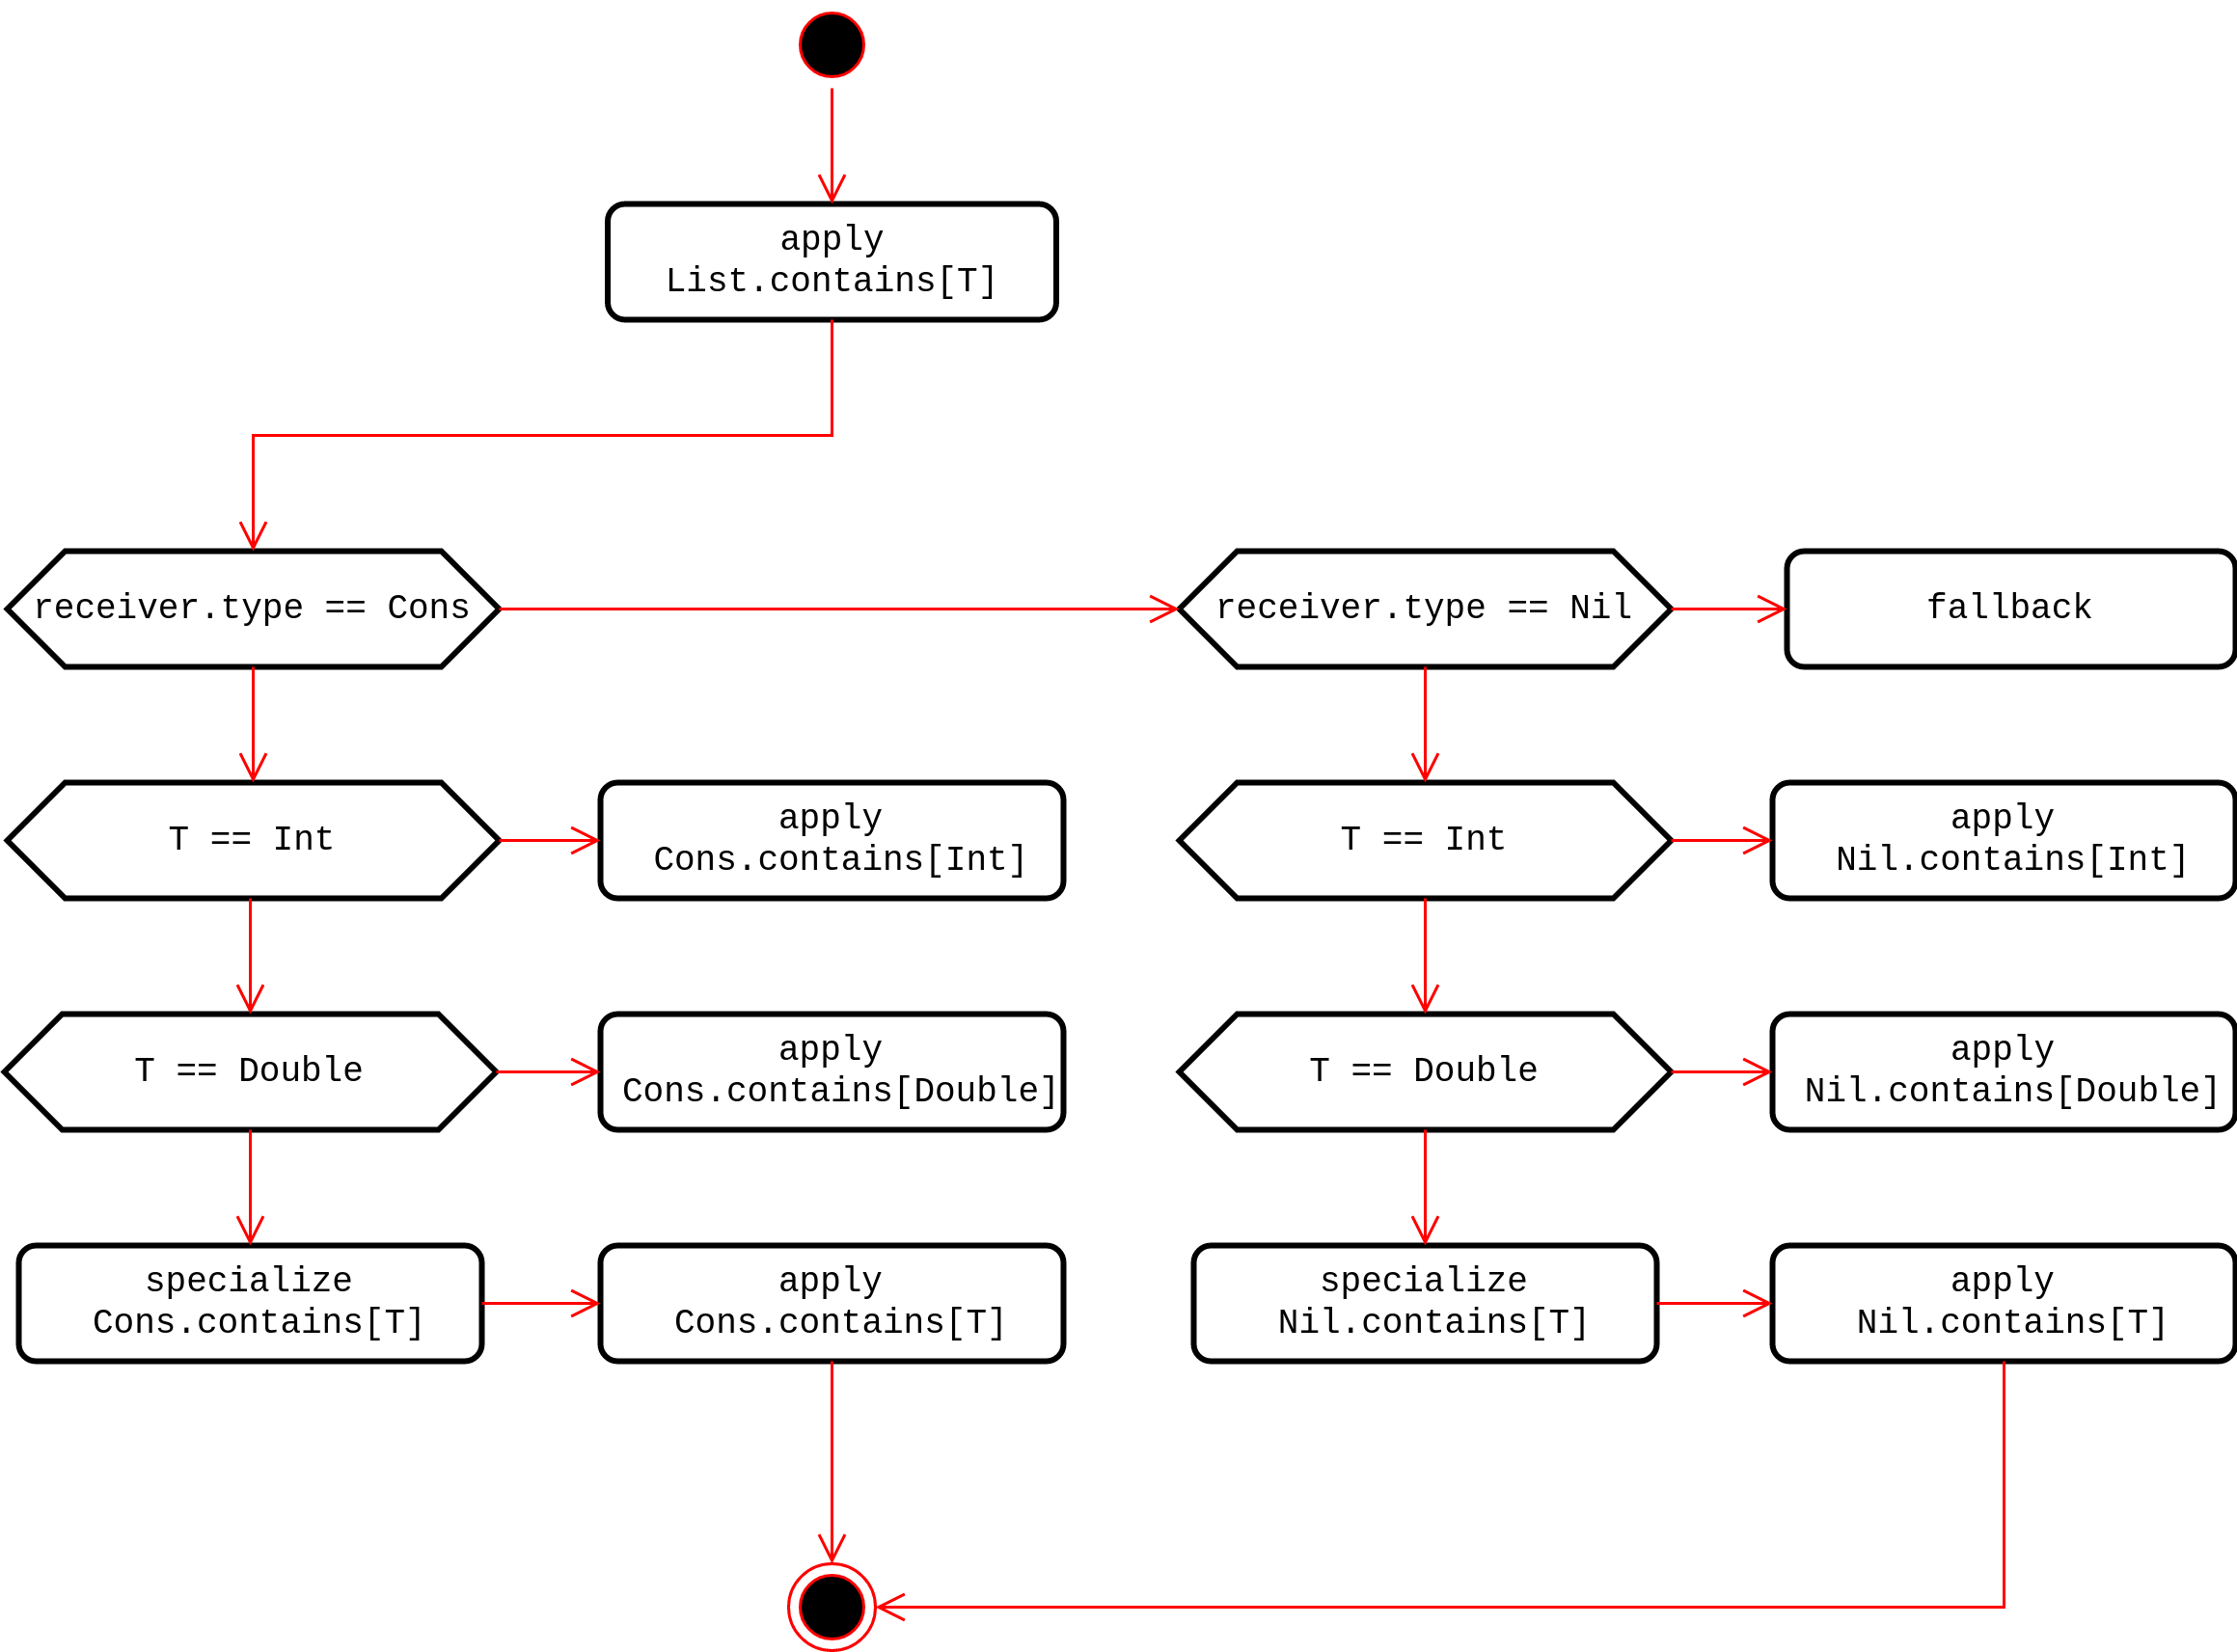
\includegraphics[width=0.75\textwidth]{figures/tastytruffle-type-dispatch-chain.png}
	\caption{The typed dispatch chain for a \scalainline{List.contains} call site}
	\label{example:typed-dispatch}
\end{figure}

Figure \ref{example:typed-dispatch} is an extension of the example given in figure \ref{example:poly-cache-call-node} with typed dispatch.
The example assumes the type arguments for \scalainline{Int} and \scalainline{Double} for \scalainline{Cons.contains[T]} and \scalainline{Nil.contains[T]} has previously been specialized and cached.
After the polymorphic inline cache resolves the receiver to an exact type, the corresponding specialization is looked up.
While this example may seem deceptively large, only the path taken in the control flow is compiled after partial evaluation.
For example, consider the invocation \scalainline{List.contains[Int]} when the receiver is an instance of \scalainline{Cons}.
The corresponding compiled code will not contain the check that type parameter is an \scalainline{Int}.
Because all other program logic is eliminated during partial evaluation, the inlining of calls is also straightforward.
After the partial evaluation, the typed dispatch mechanism is also eliminated, and the specialized method is the only code remaining.

\subsection{Case Study: The Subset of a List}

\begin{figure}[!htb]
\begin{minted}{scala}
def subsetInt(fst: List[Int], snd: List[Int]): Boolean = {
	var iter: List[T] = fst
	while (!iter.isEmpty) 
		if (!snd.contains(iter.head))
			return false 
	true
}
\end{minted}
\caption{Implementation of \scalainline{subset}.}
\label{example:list-subset}
\end{figure}

Recall the implementation of \scalainline{contains} given in figure \ref{example:cons-impl}.
An implementation of a method using \scalainline{contains} to determine if a list is the subset of another is given in \ref{example:list-subset}.
This case study is implemented for \scalainline{List[Int]} in order to showcase method specialization in the context of control flow without consideration for class specialization.
More specifically, this case study will examine how repeated invocations of \scalainline{Cons.contains[Int]} will interact with the interpreter.

In the initial execution of the \scalainline{subset} method in the interpreter, profiling information about call receiver types and type arguments are collected.
The invocation of \scalainline{contains} during the first iteration of the loop given in line $3$, the virtual call is indirect and the specialization for \scalainline{contains[Int]} does not exist.
First, the call target for the concrete implementation of \scalainline{contains} is resolved and entered into the inline cache.
Second, the specialization for \scalainline{contains[Int]} is created and entered into the inner typed inline cache.

Invocations of \scalainline{contains} in subsequent iterations of the loop where the receiver type is stable, the virtual call is inline and forwarded to the specialization for \scalainline{Int}.
Therefore, the invalidation condition in the JIT compiled variant of the code assumes the type of receiver has not changed.
Because receiver types are dynamic and type arguments are static at call sites, a change in the type of receiver at a call site is is sufficient for invalidation.
If this assumption is violated, execution resumes in the interpreter and profiling information is again collected for a future JIT compilation.

This process repeats for each receiver type seen at a call site and specialization occurs once for each of the call targets that are resolved through virtual dispatch.
Note that for $N$ possible types seen in the receiver at a call site, only $N$ specializations will be created.
The assumption generated by Truffle guard both cache lookup operations in the typed dispatch chain.
By integrating typed dispatch into an inner inline cache after virtual call resolution, no additional assumptions are generated by Truffle for JIT compilation.

\subsection{Specializing Polymorphic Parameters}

The data layout of a method is given by the frame descriptor of its root node.
A specialized method will have a specialized frame descriptor.
Specialized frame descriptors will have the appropriate primitive frame slot kinds assigned to value definitions that have their polymorphic types resolved to a primitive type.
Therefore, the core principle behind method specialization is generating a \scalainline{TermNode} tree from a \scalainline{Term} tree using a specialized frame descriptor.
Apart from extensions given earlier in this section, the parsing of \scalainline{Term} nodes does not differ from their monomorphic counterparts.

Figure \ref{impl:gen-poly-locals} gives an extension to generate frame slots from type parameters and polymorphic value definitions associated with the method to generate frame slots from monomorphic value definitions.
Like its counterpart in the monomorphic interpreter, the abstraction for a local frame value in the polymorphic interpreter has a slot.
However, a local frame value in the polymorphic interpreter retains a type instead of a frame slot kind.
If the type of a value parameter can be resolved with the type arguments supplied during specialization, the specialized frame slot is created and added to the descriptor.

\begin{figure}[!htb]
\begin{minted}{scala}
class DefDefTemplate(...) extends RootNode(...) {
	def execute(frame: VirtualFrame): Object = ...
		
	def specialize(types: Array[Type]): DefDefNode = {
		val desc = this.desc.copy()
			
		val parameters = self :: vparams.map(specializeValDef(types, desc))
		locals.foreach(specializeValDef(types, desc))
			
		val body = parse(rhs)
		new DefDefNode(desc, parameters, body)
	}

	def specializeValDef(
		types: Array[Type], 
		desc:  FrameDescriptor, 
		v:     LocalFrameVal | ValDef
	): LocalFrameVal = v match {
		case vdef: ValDef => generateLocal(types, vdef, desc)
		case v => v
	}
}
\end{minted}
\caption{Pseudocode for on-demand specialization inside a \scalainline{DefDefTemplate}.}
\label{impl:defdeftemplate-specialize}
\end{figure}

$$
index(\tau) = 
\begin{cases}
	i  & \textbf{def } f[t_0, \ldots, t_i, \ldots, t_n](\ldots) \text{ if } t_i = \tau, owner(\tau)=f \\
	-1 & \text{otherwise}
\end{cases}
$$

Figure \ref{impl:defdeftemplate-specialize} contains the pseudocode for creating specialized root nodes and accompanying frames using type arguments.
A mapping of types (via their symbols) to their respective index in the type argument array is sufficient to handle this resolution.
The symbol \textit{owner} is the symbol of the tree that encloses the current tree.
Because we are only discussing methods polymorphic under their own type parameters, all polymorphic value parameters are resolved in this context.
The derivation of local frame values from monomorphic value definitions remains unchanged. 

\begin{figure}[!htb]
\begin{minted}{scala}
def generateLocal(types: Array[Type], defn: ValDef | TypeDef, desc: FrameDescriptor): LocalFrameVal = 
	defn match {
		case tdef: TypeDef => 
			val kind = FrameSlotKind.Object
			val slot = desc.addSlot(kind)
			LocalFrameVal(slot, ReifiedType)
		case vdef: ValDef => 
			val idx  = index(vdef.tpt.tpe)
			val tpe  = if (idx != -1) types(idx) else vdef.tpt.tpe
			val kind = getFrameSlotKind(tpe)
			val slot = desc.addSlot(kind)
			LocalFrameVal(slot, tpe)
	}
\end{minted}
\caption{Extension to pseudocode that generates frame slots to include polymorphic definitions.}
\label{impl:gen-poly-locals}
\end{figure}

A type definition is treated in the same manner as a value definition; it is assigned a frame slot with an \javainline{Object} frame slot kind.
This allows storing types in the method frame, allowing for the resolution of types after invoking a method template.
So far, we have only discussed the resolution of type arguments in an intraprocedural context.
Storing reified types in the frame during execution allows for the resolution in an interprocedural context.
We will detail why this is important in the following subsection.

Truffle conveniently profiles the types of frame arguments to speculatively eliminate the unboxing of boxed values when reading frame values (including arguments). 
For example, the following invocation \scalainline{list.contains((elem: Int))} will be profiled by Truffle even if we store \scalainline{elem} in an \scalainline{Object} frame slot.
Truffle will then speculatively unbox \scalainline{elem} in the body of \scalainline{contains} if appropriate.
These optimizations and their limits are discussed in Chapter \ref{chapter:evaluation}.

\begin{figure}[!htb]
\begin{minted}{scala}
def maximum[T <: Numeric](list: List[T]): Boolean =  {
	var max: T  = zero
	var curr: List[T] = a
	while (!curr.isEmpty) 
		if (curr.head > max)
			max = curr.head 
	max
}
\end{minted}
\caption{Implementation of a \texttt{max} method for a \scalainline{List}.}
\label{impl:list-max}
\end{figure}

In contrast, write operations of polymorphic frame values cannot be speculatively eliminated. 
Because Truffle does not specialize data layouts, i.e., frames are determined by their descriptors, which in turn are determined by the guest language implementation, frame writes of polymorphic values will always have to be boxed.
The elimination of boxed polymorphic writes from frame descriptor specialization is one of the major benefits when compared to the monomorphic interpreter.
Code that has polymorphic code, which reads and writes to a frame frequently, will no longer have to unbox, compute primitive operations on unboxed values, then box those values back into their respective slots.
Figure \ref{impl:list-max} contains an example program with polymorphic code that frequently writes to a polymorphic local variable after some computation.

\subsection{Case Study: A List Constructor}

\begin{figure}[!htb]
\begin{minted}{scala}
object List {
	def apply[T](array: Array[T]): List[T] = {
		var i = array.length - 1
		var these: List[T] = Nil
		while (i >= 0) {
			these = new Cons[T](array(i), these)
			i -= 1
		}
		these
	}	
}
\end{minted}
\caption{An alternate static constructor that converts an \scalainline{Array[T]} to a \scalainline{List[T]}}
\label{impl:list-alt-constructor}
\end{figure}

In this section, we examine an example containing code Truffle cannot optimize well.
Figure \ref{impl:list-alt-constructor} gives an additional constructor that creates a polymorphic list from a polymorphic array.
We focus on the term \scalainline{array.length}, which computes the length for a polymorphic array on line $3$.
When the Typer detects an array operation on a polymorphic array value, it automatically inserts the array runtime bridge method responsible for handling the operation.
For example, line $3$ after the Typer would be transformed into \scalainline{var i = array_length(array) - 1}.
We give the implementation of \scalainline{array_length} in figure \ref{impl:array-length}.

\begin{figure}[!htb]
\begin{minted}{scala}
def array_length(array: AnyRef): Int = {
	if (array.isInstanceOf[Array[AnyRef]])       array.asInstanceOf[Array[AnyRef]].length
	else if (array.isInstanceOf[Array[Int]])     array.asInstanceOf[Array[Int]].length
	else if (array.isInstanceOf[Array[Double]])  array.asInstanceOf[Array[Double]].length
	else if (array.isInstanceOf[Array[Long]])    array.asInstanceOf[Array[Long]].length
	else if (array.isInstanceOf[Array[Float]])   array.asInstanceOf[Array[Float]].length
	else if (array.isInstanceOf[Array[Char]])    array.asInstanceOf[Array[Char]].length
	else if (array.isInstanceOf[Array[Byte]])    array.asInstanceOf[Array[Byte]].length
	else if (array.isInstanceOf[Array[Short]])   array.asInstanceOf[Array[Short]].length
	else if (array.isInstanceOf[Array[Boolean]]) array.asInstanceOf[Array[Boolean]].length
	else throw new NullPointerException
}
\end{minted}
\caption{Implementation of \scalainline{array_length}}
\label{impl:array-length}
\end{figure}

In both Scala and the JVM, arrays of primitive types are invariant.
That is to say, the type \scalainline{Array[Int]} is neither a subtype or supertype of the type \scalainline{Array[Any]}.
On the other hand, the type \scalainline{Array[T <: AnyRef]} is covariant.
This contradiction in the presence of code that creates or operates on polymorphic arrays requires runtime bridge methods to appear seamless to a programmer.
When combined with the nature of Scala's type system, the Scala runtime obscures opportunities for speculative optimizations.

Notice the type of the argument in \scalainline{array_length} is \scalainline{AnyRef}; because the types of arrays are invariant, the direct supertype is \scalainline{AnyRef}, the type for any reference type.
To compute the length for a polymorphic array, \scalainline{array_length} switches over every similar but unrelated array type.
In the body of every type check condition, the argument must be cast to the appropriate array type after the type check succeeds before the length is finally computed.
We introduce a method to vastly simplify the Graal IR of such instances of array bridge methods when specialized methods would have type-specific information to augment JIT compilation.

\begin{figure}[!htb]
\begin{minted}{scala}
import CompilerDirectives.castExact
def copyArgumentsToFrame(frame: VirtualFrame): Unit = 
	for ((param, arg) <- params zip frame.getArguments) 
		param.tpe match {
			case Int =>
				frame.setInt(param.slot, arg.asInstanceOf[Int])
				...
			case Double =>
				frame.setDouble(param.slot, arg.asInstanceOf[Double])	
			case tpe: Array[AnyRef] | tpe: Array[Int] | ... | tpe: Array[Double] =>
				frame.setObject(param.slot, castExact(arg, getClass(tpe)))
			case _ =>
				frame.setObject(param.slot, arg)
		}
\end{minted}
\caption{Pseudocode for \scalainline{DefDefNode} and \scalainline{Parameter}}
\label{impl:specialized-copy-arguments}
\end{figure}

As arrays are references, they are stored on frames via an \scalainline{Object} slot.
This alone is insufficient to optimize polymorphic frame slots for array types.
Instead, we extend the way that frame arguments are copied into the frame from figure \ref{impl:defdefnode} in figure \ref{impl:specialized-copy-arguments}.
Because a parameter now retains its type instead of a frame slot kind, we introduce a special operation when copying arguments that are arrays. 
The \javainline{castExact} directive is a type narrowing operation that hints to Graal that a value is an instance of a type.
By injecting type information from TASTy into our executable IR, all subsequent checks that switch over the type of an array are simplified during partial evaluation.

\subsection{Propagating Type Arguments}

\begin{figure}[!htb]
\begin{minted}{scala}
def subset[T](a: List[T], b: List[T]): Boolean = {
	var curr: List[T] = a
	while (!curr.isEmpty) {
		if (!b.contains[T](curr.head)) return false
		curr = curr.tail
	}
	true 
}
\end{minted}
\caption{An example where type arguments are derived from type parameters.}
\label{impl:list-subset}
\end{figure}

Polymorphic invocations often occur inside the definition of a polymorphic class or a polymorphic method.
That is to say that, the type argument at a type application site can be a type parameter.
Figure \ref{impl:list-subset} is an example where a type application occurs inside the definition of a polymorphic method and derives its type argument from a type parameter.

\begin{figure}[!htb]
\begin{minted}{scala}
class MethodParamTypeNode(@Child readLocal: ReadLocalNode) extends TypeNode {
	override def resolveType(frame: VirtualFrame): Type = 
		readLocal.execute(frame).asInstanceOf[Type]
}
\end{minted}
\caption{The type node for dynamically resolving method type parameters.}
\label{impl:method-param-typenode}
\end{figure}

We introduce a subclass of a type node that retrieves method type arguments stored on the frame.
Because type parameters are treated in the same manner as value parameters, they are stored in the method's frame.
The resolution of type arguments that are parameters from a method follows the same mechanism as the resolution of local variables.
This mechanism enjoys the same Truffle virtualization optimizations of value reads when propagating type arguments interprocedurally.
Subsequent invocations of polymorphic methods that have type parameters stored on the frame will partial evaluate their specializations.

\section{Specializing Classes}

\begin{figure}[!htb]
\begin{minted}{scala}
def parseClassDef(cdef: ClassDef, types: Array[Type]]): ClassShape = {
	val parents = cdef.parents.map(_.symbol)
		
	val fields = cdef.body map {
		case vdef: ValDef => generateField(vdef, types)	
	}
	
	val methods = (cdef.constructor :: cdef.body) map {
		case ddef: DefDef => ddef.symbol.signature -> parseDefDef(ddef)
	}
		
	val vtable = cdef.symbol.methodMembers map {
		symbol => symbol.signature -> symbol
	}
		
	new ClassShape(cdef.symbol, parents, fields, init ++ methods, vtable)
}
\end{minted}
\caption{Extensions to specialize a \scalainline{ClassDef}.}
\label{impl:specialize-class}
\end{figure}

This section details the specialization of classes and class members with polymorphic semantics based on class type parameters.
Previously, we discussed the specialization of methods that are solely polymorphic under their parameters without the mention of methods that are class-polymorphic.
The reasoning behind this decision can be explained thus: the invocation of a class-polymorphic method requires a look up into that class's shape; by extension, that class must be specialized before such a polymorphic invocation may occur.
For example, the method \scalainline{List.contains} in figure \ref{example:list-def} contains method-polymorphic semantics that are resolved \textit{after} a polymorphic class instance is created.

As class specialization does not share the same demands regarding runtime mechanisms as method specialization, we will adopt a rewrite-driven approach to specializing class definitions at object creation sites.
We will use techniques to monomorphize, at least partially, polymorphic TASTy trees instead of altering the transformation of a \scalainline{ClassDef} to a \scalainline{ClassShape}.
With this rationale, we can adapt many elements of the monomorphic interpreter for polymorphism.

\begin{figure}[!htb]
\begin{minted}{scala}
class ClassParamTypeNode(@Child readField: ReadFieldNode) extends TypeNode {
	override def resolveType(frame: VirtualFrame): Type = 
		readLocal.execute(frame).asInstanceOf[Type]
}
\end{minted}
\caption{The type node for dynamically class method type parameters.}
\label{impl:class-param-typenode}
\end{figure}

Figure \ref{impl:specialize-class} provides an overview of the steps that are required to create a specialized monomorphic \scalainline{ClassDef} from a polymorphic origin.
Similar to how type definitions become parameters when reified in the context of a \scalainline{DefDef}, type definitions in the context of \scalainline{ClassDef} become fields when reified.
The rationale is that instances of specialized polymorphic classes store their specialized type fields to propagate types.
Figure \ref{impl:class-param-typenode} gives the pseudocode for a type node that resolves a type parameter from an instance of a specialized class.
We rewrite both value and method definitions to transform polymorphic class definitions into monomorphic class definitions.

\subsection{Creating Specialized Instances}

\begin{figure}[!htb]
\begin{minted}{scala}
parseType(tpe: Type): TypeNode = tpe match {
	...
	case AppliedType(con, targs) => 
		new AppliedTypeNode(parseType(con), targs map parseType) 
}

class AppliedTypeNode(	
	@Child con: TypeNode, 
	@Children targs: Array[TypeNode]) extends TypeNode {
	@ExplodeLoop
	override def resolve(frame: VirtualFrame): Type {
		val types = Array.empty[Type]
		for (targ <- targs)
			types += targ.resolve(frame)
		
		AppliedType(con.resolve(frame), types)
	}
}

def shapeOf(tpe: Type): ClassShape = tpe match {
	...
	case AppliedType(con, targs) => 
		val cdef = getClassDef(con)
		parseClassDef(cdef, targs)
}
\end{minted}
\caption{The \scalainline{AppliedTypeNode} and its derivation from an \scalainline{AppliedType}.}
\label{impl:applied-type-node}
\end{figure}

The \scalainline{AppliedType} is the analogue of \scalainline{TypeApply} for type applications when creating object instances.
We can derive a specialization site for class definition by the reification of an applied type into an \scalainline{AppliedTypeNode}.
Figure \ref{impl:applied-type-node} is an overview of the \scalainline{AppliedTypeNode} and its derivation from its TASTY type counterpart.
In our subset of TASTy, an applied type represents an instantiation of a polymorphic type.

\begin{figure}[!htb]
\begin{minted}{scala}
new List[Int]
\end{minted}
\caption{Example of creating instance of an applied type.}
\label{example:applied-type}
\end{figure}

For example, consider the term, given in figure \ref{example:applied-type}, that returns an instance of a polymorphic type.
The type \scalainline{List[Int]} is the result of the type application of \scalainline{List[T]} to \scalainline{Int}.
We will refer to polymorphic applied types, such as \scalainline{List[T]}, as \textit{polymorphic} applied types. 
The data representation of a polymorphic applied type is undetermined; depending on the type arguments supplied during type application, the data representation will vary.

\begin{figure}[!htb]
\begin{minted}{scala}
NewNode(AppliedTypeNode(TypeRefNode("List"), Array(TypeRefNode("Int"))))
\end{minted}
\caption{TastyTruffle IR of creating an instance of an applied type.}
\label{example:applied-type-node}
\end{figure}

When executable nodes are derived from polymorphic applied types, given in figure \ref{example:applied-type-node}, type arguments are resolved during runtime before application to their type constructor.
We refer to the instantiations resulting from the application of type arguments to polymorphic applied types as \textit{monomorphic} applied types (e.g., List[Int]).
Having a monomorphic applied type provides the opportunity to generate a specialized shape.
Therefore, each group of monomorphic applied types has a unique data representation.
For example, a \scalainline{List[Int]} and \scalainline{List[Double]} will each have a unique data representation, and the underlying layout of their instances will be different.
However, a \scalainline{List[String]} and \scalainline{List[List[Int]]} will share the same data representation as their type arguments are reference types and will not see any benefit from independent specialization.
Therefore, creating an object instance with a polymorphic class definition will have its shape determined when its created.

This approach also avoids the issue of \textit{name mangling}.
Name mangling disambiguates distinct entities in a program that share the same name but do not inhabit the same namespace (e.g., a \javainline{package}).
In the context of parametric polymorphism and specialization, many approaches to specialization require specialized classes and methods to have mangled names.
The creation of polymorphic classes and call sites of polymorphic methods must be rewritten to refer to the correct specialization.
In our approach, operations on object instances with a polymorphic type are unaffected by its underlying shape.
In the next section, we give extensions on generating a static shape from a monomorphic applied type after type application.

\subsection{Case Study: \texttt{Cons.head}}

\begin{figure}[!htb]
\begin{minted}{scala}
val list: List[Int] = ...
list.contains(0)
\end{minted}
\caption{Example invocation of \scalainline{Cons.contains[Int]}}
\label{example:list-contains-example}
\end{figure}

In this section, we introduce an example, given in figure \ref{example:list-contains-example}, that motivates the specialization of shapes.
The example is a source-like representation of \scalainline{List.contains[Int]}, the specialized variant of the \scalainline{List.contains} method.
We compare the body of \scalainline{List.contains} with and without a specialized storage layout for the implementation of \scalainline{contains} in the \scalainline{Cons} class.

\begin{figure}[!htb]
\begin{minted}{scala}
def contains$Int(elem: Int): Boolean = {
	var these: List = this
	while (!these.isEmpty) {
		val head = these.head.asInstanceOf[Int]
		if (unbox(head) == elem) return true
		else                     these = these.tail
	}
	false
}	
\end{minted}
\caption{Implementation of \scalainline{contains} in an erased \scalainline{Cons} class.}
\label{impl:cons-contains-erased}
\end{figure}

Figure \ref{impl:cons-contains-erased} contains a source-like representation of \scalainline{contains} if the data layout of \scalainline{Cons} follows the standard translation of type erasure but the method is still specialized.
We draw attention to the example's equality operation defined on line $5$.
Without the specialization of either classes or methods, both the left-hand-side and right-hand-side operands would be boxed integers, and the \scalainline{==} operation dispatches to \scalainline{these.head.equals(elem)}.
However, because methods are specialized and classes are not specialized in our case, the \scalainline{head} field must be unboxed before equality can be checked.
Figure \ref{impl:cons-contains-specialized} contains the specialized equivalent code of \ref{impl:cons-contains-erased}.
Once the class layout is specialized, no unboxing is present in the program.

\begin{figure}[!htb]
\begin{minted}{scala}
def contains$Int(elem: Int): Boolean = {
	var these: List = this
	while (!these.isEmpty) {
		// val head = ...
		if (these.head == elem) return true
		else these = these.tail
	}
	false
}	
\end{minted}
\caption{Implementation of \scalainline{contains} in a specialized \scalainline{Cons} class.}
\label{impl:cons-contains-specialized}
\end{figure}

\subsection{Specializing Class Members}

\begin{figure}[!htb]
\begin{minted}{scala}
def generateField(vdef: ValDef, types: Array[Type]): Field = vdef match {
	case ValDef(_: String, tpt: TypeTree, rhs: Option[Term]) => 
		val idx = index(tpt.tpe)
		val tpe = if (idx > 0) types(idx) else tpt.tpe
		new Field(vdef.symbol, tpe)
}
\end{minted}
\caption{Extensions to generate a field from a polymorphic value definition.}
\label{impl:generate-poly-field}
\end{figure}

This section extends the translation scheme for generating shapes from class definitions to include polymorphic class definitions.
There are two elements of data layout that must be determined when generating the shape of a polymorphic class definition.
Fields, the data in object instances, must be resolved with monomorphic types for value definitions.
Frame slots, data stored in the frame of methods that are class-polymorphic, must also be resolved.
Frame slots and descriptors present a unique challenge as complete specialization of descriptors may require type parameters from both methods and classes.

The underlying type of a polymorphic field, and therefore its data representation as part of its static shape, cannot be determined statically.
When the field translation scheme is supplied with type arguments, we can generate the specialized monomorphic field.
Figure \ref{impl:generate-poly-field} extends the pseudocode that generates fields for shapes to include polymorphic value definitions.
If it is beneficial to specialize a field, e.g. \scalainline{val x: T} or \scalainline{val x: Array[T]}, we resolve the type parameter from the type arguments to generate a specialized field property.
Otherwise, we default to the monomorphic implementation for generating a field.

\begin{figure}[!htb]
\begin{minted}{scala}
def parseDefDef(ddef: DefDef, types: Array[Type]): DefDefNode | DefDefTemplate = {
	val tparams = ddef.params.filter(_.isInstanceOf[TypeDef]).length
	
	val vparams = ddef.filter(_.isInstanceOf[ValDef]) map {
		case vdef @ ValDef(_, tpt, rhs) => specializeValDef(desc, vdef, types))
	}

	val locals = liftLocals(ddef.rhs) map {
		case vdef @ ValDef(_, tpt, rhs) => specializeValDef(desc, vdef, types))
	}
	
	val noGenParams = vparams.forall(_.isInstanceOf[LocalFrameVal]
	val noGenLocals = locals.forall(_.isInstanceOf[LocalFrameVal])
	if (noGenParams && noGenLocals)
		new DefDefNode(desc, vparams, ddef.rhs)
	else 
		new DefDefTemplate(desc, tparams, vparams, locals, ddef.rhs)
}
\end{minted}
\caption{Extension to parse a \scalainline{DefDef} with class type arguments.}
\label{impl:parse-poly-defdef-cls}
\end{figure}

Polymorphic methods challenge specialization because they can be polymorphic under two sets of type parameters.
As a result, dynamically resolved types are not available for specialization at the \textit{same} time; class type arguments are available at object creation, and method type arguments are available at invocation.
To address this, we need to be able to \textit{partially specialize} methods from the class perspective.
Figure \ref{impl:parse-poly-defdef-cls} extends the translation of \scalainline{DefDef} nodes with class type arguments.
If the method is polymorphic under class type parameters, the layout of a frame for the root node of a \scalainline{DefDef} must be partially determined.

$$
index(\tau) = 
\begin{cases}
	i  & \textbf{def } f[t_0, \ldots, t_i, \ldots, t_n](\ldots) \text{ if } t_i = \tau, owner(\tau)=f \\
	j  & \textbf{class } C[t_0, \ldots, t_j, \ldots, t_m](\ldots) \text{ if } t_j = \tau, owner(\tau)=C \\
	-1 & \text{otherwise}
\end{cases}
$$

We extend the definition of \scalainline{index} to resolve the index of a type parameter to a corresponding type argument array in a context-sensitive manner (i.e., whether type arguments originate from a type application of a class or a method).

After the class specialization of a \scalainline{DefDef}, it is still possible that a \scalainline{DefDef} contains polymorphic semantics.
However, all polymorphism that is derived from a class type parameter has been specialized, and such terms and parameters are now monomorphic.
Therefore, a \scalainline{DefDef} that is still polymorphic is only polymorphic under its own type parameters.
The remaining polymorphic data layout will be specialized when the method template is invoked.

\begin{figure}[!htb]
\begin{minted}{scala}
ClassShape(
	"Cons$Int",
	Array(
		Field("T", Object),
		Field("head", Int),
		Field("tail", Object)
	),
	Map(
		"length()"               -> DefDefNode("length")
		"contains[1](scala.Any)" -> DefDefTemplate("contains")
		"hashCode()"             -> DefDefNode("hashCode")
	
	),
	...
)
\end{minted}
\caption{Shape of \scalainline{Cons[Int]}}
\label{shape:cons-int}
\end{figure}

As an example, we give figure \ref{shape:cons-int} to show the data layout of the specialized class \scalainline{Cons[Int]}.
We omit the runtime elements of a shape in our example as we only want to show how the data of a specialized shape is organized.
The only object storage property that differs between class specializations is the \scalainline{head} field.
For the specialization \scalainline{Cons[Int]}, the \scalainline{head} field is stored with the \scalainline{Int} type.
The storage types of fields may differ among specializations; they are all referenced by the same symbol.
This allows the access of fields between specializations to remain opaque from the perspective of client code.

The layout of the shape with respect to call targets remains unchanged.
Call targets are duplicated across each shape of a specialized class definition.
Because method definitions potentially contain polymorphic code that relies on class type parameters, this duplication is necessary for each class-specialized call target to have the correct frame descriptor.

Each specialized shape contains fields that store the type argument of their specialization.
These remain constant throughout all instances of the same specialized shape, allowing us to store the type arguments on shapes directly.
Having type parameters as fields allow the reuse of the field access interface for class type definitions.

%======================================================================
\chapter{Evaluation}
\label{chapter:evaluation}
In this chapter, The performance of the polymorphic interpreter will be evaluated on six microbenchmarks.
An existing set of benchmarks from \cite{scala:miniboxing} will be used as they exercise many features of the Scala runtime that require specialization to perform optimally.
The performance of these benchmarks will also be evaluated on the monomorphic interpreter, the variant of our interpreter that does not specialize data layout, to measure the improvement produced by our techniques. 
The benchmarks will also be evaluated on native Scala bytecode executing on GraalVM to demonstrate the results produced by \textsc{TastyTruffle} are fair when compared to a real world implementation.
Finally, we discuss the results of the benchmarks, examine the causes of performance deficiencies, and how our implementation resolves them.

\section{Benchmarks}

In this section, we will introduce an additional program on top of our running example for benchmarking.
We will also summarize the motivations for selecting these benchmarks from \cite{scala:miniboxing}.

Each microbenchmark exercises unique polymorphic operations that are typically performance bottlenecks\cite{scala:collections-optimization,scala:dacapo} in Scala programs.
The \scalainline{ArrayBuffer} class implements a resizable buffer backed by an array.
It contains three microbenchmarks that stress polymorphic operations in the context of contiguous memory access.

The \scalainline{List} class is the implementation of a linked list that we have used as the running example in this thesis.
We use the \scalainline{List} class to evaluate polymorphic operations in the context of random heap access.
Like the \scalainline{ArrayBuffer} benchmarks, there is an \scalainline{append} and \scalainline{contains} microbenchmark.
We will use lists to test the performance of polymorphic hash computations using \scalainline{List.hashCode}.

\begin{figure}[!htb]
\begin{minted}{scala}
class ArrayBuffer[T] {
	protected def initialSize: Int = 16
	var size0 = 0
	var array: Array[T] = newArray[T](Math.max(initialSize, 1))
	
	def length: Int = size0
	private def get(i: Int): T = array(i)
	private def set(i: Int, elem: T): Unit = array(i) = elem
	
	def contains(elem: T): Boolean = {
		var i = 0
		while (i < size0) {
			if (array(i) == elem) return true
			i += 1
		}
		false
	}
	
	def reverse(): Unit = {
		var pos = 0
		while (pos * 2 < size0) {
			swap(pos, size0 - pos - 1) // swaps two elements in the array
			pos += 1
		}
	}
	
	def append(elem: T): Unit = {
		val newSize0 = size0 + 1
		ensureSize(newSize0)
		set(size0, elem)
		size0 = newSize0
	}
	

\end{minted}
\caption{Code of the \scalainline{ArrayBuffer} benchmark.}
\label{example:arraybuffer-benchmark}
\end{figure}

\section{Methodology}

Performance measurement of just-in-time compiled programs is an infamously difficult issue\cite{java:performance-analysis,java:statistically-rigor-performance-analysis}.
Many non-deterministic effects, such as speculative optimization, garbage collection, and thread scheduling, affect the performance of programs executing on the Java Virtual Machine.
As a result, the JVM must be \textit{warmed up} before measuring program performance.
A benchmarking routine is warmed up with several iterations of invocations for profiling data to be collected and JIT compilation to be finished.
Therefore the measured performance of a microbenchmark will record the program executing the stable JIT compiled code instead of code executing in the interpreter.

Each benchmark method in this chapter is warmed up with $10$ iterations of warmup lasting $10$ seconds each.
Results of these are measured in throughput, the number of executions that were successfully completed in a second.
The results are averaged from $10$ measurement iterations for $10$ seconds each.
We evaluate our microbenchmarks on input sizes between one hundred thousand and one million elements to account for memory factors in our benchmarks. 
Each benchmark is run on three different implementations, Scala on GraalVM (Graal), the monomorphic interpreter without specialization (Mono), and the polymorphic interpreter (Poly).
While we provide the evaluation of our benchmarks on Scala and GraalVM, we do so to provide a baseline to show that the performance of our monomorphic interpreter is reasonable and that the performance improvement of our polymorphic extensions is fair.

\section{Experimental Results}

\begin{figure}
	\centering
	\includesvg[height=0.9\textheight]{data/ArrayBuffer.Append.svg}
	\caption{Benchmark results for \scalainline{ArrayBuffer.append}.}
	\label{results:array-append}
\end{figure}

\begin{figure}
	\centering
	\includesvg[height=0.9\textheight]{data/ArrayBuffer.Contains.svg}
	\caption{Benchmark results for \scalainline{ArrayBuffer.contains}.}
	\label{results:array-contains}
\end{figure}

\begin{figure}
	\centering
	\includesvg[height=0.9\textheight]{data/ArrayBuffer.Reverse.svg}
	\caption{Benchmark results for \scalainline{ArrayBuffer.reverse}.}
	\label{results:array-reverse}
\end{figure}

\begin{figure}
	\centering
	\includesvg[height=0.9\textheight]{data/List.Append.svg}
	\caption{Benchmark results for \scalainline{List.append}.}
	\label{results:list-append}
\end{figure}

\begin{figure}
	\centering
	\includesvg[height=0.9\textheight]{data/List.Contains.svg}
	\caption{Benchmark results for \scalainline{List.contains}.}
	\label{results:list-contains}
\end{figure}

\begin{figure}
	\centering
	\includesvg[height=0.9\textheight]{data/List.Hashcode.svg}
	\caption{Benchmark results for \scalainline{List.hashCode}.}
	\label{results:list-hashcode}
\end{figure}

\begin{figure}[!htb]
\begin{minted}{scala}
// Ensure that the internal array has at least `n` cells. 
def ensureSize(n: Int): Unit = {
	val arrayLength: Long = array.length // Use a Long to prevent overflows
	if (n > arrayLength) {
		var newSize: Long = arrayLength * 2
		while (n > newSize) newSize = newSize * 2
		// Clamp newSize to Int.MaxValue
		if (newSize > lang.Int.MaxValue) newSize = lang.Int.MaxValue
		
		val resized = newArray[T](newSize.toInt)
		var i = 0
		while (i < size0) {
			resized(i) = get(i)
			i += 1
		}
		array = resized
	}
}	
\end{minted}
\caption{Implementation of \scalainline{ensureSize} of the \scalainline{ArrayBuffer} benchmark.}
\label{example:arraybuffer-resize}
\end{figure}

The benchmark for \scalainline{ArrayBuffer.append} inserts a sequence of elements into a newly initialized array buffer. 
This benchmark stresses array memory movement and the results are given in figure \ref{results:array-append}.
Each time the backing array is too small for an additional element, the backing array is resized by creating a new larger array and copying over existing elements.
This resizing operation (\scalainline{ensureSize} in \ref{example:arraybuffer-resize}) dominates the time spent in execution.
There are autoboxing operations that occur during the update of the backing array when appending an element.
As such, appending to an array buffer is on average $1.5$ times faster on the polymorphic interpreter than the monomorphic interpreter.
However, the time spent in this benchmark is dominated by the array resizing operation, which largely translates to memory allocation and movement.
Because of this, executing compiled Scala bytecode on GraalVM can be up to $4$ times faster than the monomorphic and polymorphic interpreter for smaller input sizes.
These types of operations are faster executing in Java bytecode on Graal when compared to a Truffle interpeter.
However, as input size grows, the gap in throughput between Scala on GraalVM and polymorphic TastyTruffle narrows.

The \scalainline{ArrayBuffer.contains} benchmark tests array operations in isolation. 
The benchmark checks an array buffer for the existence of an element and the results are given in figure \ref{results:array-contains}.
It exercises a polymorphic array access followed by a polymorphic equality operation (e.g. \scalainline{(x: T) == (y: T)}).
A polymorphic equality operator has dispatched the \javainline{equals} method of its left-hand side argument.
This results in boxing one or both arguments in equality checks between polymorphic values.
The specialization of the \scalainline{List.head} field and the subsequent specialization of \scalainline{Any.==} into the appropriate value equivalent resulted in an average $4$ times greater throughput for long values, $3.6$ times greater throughput  speedup for double values, and $3$ times greater throughput for int values.

\scalainline{ArrayBuffer.reverse} reverses the order of the elements in the array buffer.
Reversing an array is performance-bound by the loop of swap operations.
A swap operation (given in \ref{impl:swap}) consists of two polymorphic value definitions (frame writes) initialized from polymorphic array accesses followed by the inverse of those two operations.

\begin{figure}[!htb]
\begin{minted}{scala}
def swap(i: Int, j: Int): Unit = {
	val tmp1: T = get(i)
	val tmp2: T = get(j)
	set(i, tmp2)
	set(j, tmp1)
}
\end{minted}
\caption{Code to swap two elements in an array buffer}
\label{impl:swap}
\end{figure}

The performance of the \scalainline{reverse} microbenchmark proved to be the most challenging benchmark in terms of matching handwritten monomorphic code in \cite{scala:miniboxing}.
The performance of each type variant of \scalainline{reverse} is roughly equal in the monomorphic interpreter and Scala on GraalVM; neither implementation can specialize the polymorphic reads and array accesses.
The polymorphic interpreter has up to $28$ times more throughput than the monomorphic interpreter and GraalVM.

The \scalainline{List.append} benchmark constructs a list from an array.
As the creation of polymorphic instances is predominantly memory-bound and not compute-bound, there is no significant improvement in throughput from specialization.
In fact, executing Scala via Java bytecode on the JVM results in substantially greater throughput.
Appending to a list on Graal is up to $8$ faster than the monomorphic and polymorphic interpreter.

\scalainline{List.contains} exercises the same performance-bottlenecks as \scalainline{ArrayBuffer.contains}, except under the context of random heap access for a list.
The execution of \scalainline{List.contains} on the polymorphic interpreter is roughly $50\%$ faster than on the monomorphic interpreter.

\scalainline{List.hashCode} tests the specialization of the hash code function.
Every class in Scala inherits the \scalainline{hashCode} function from the \scalainline{Any} type.
When the \scalainline{hashCode} method is invoked in a polymorphic context, the Scala compiler inserts the \scalainline{anyHash} bridge.
The semantics of computing hash codes among the same values with different types, such as \scalainline{Int} and \scalainline{Long}, necessitates the insertion of this bridge, which complicates JIT compilation.

\begin{figure}[!htb]
\begin{minted}{java}
public static int anyHash(Object x) {
	if (x == null)           return 0;
	if (x instanceof Long)   return longHash(((Long) x).longValue());
	if (x instanceof Double) return doubleHash(((java.lang.Double) x).doubleValue());
	if (x instanceof Float)  return floatHash(((Float) x).floatValue());
	
	return x.hashCode();
}
\end{minted}
\caption{Implementation of the \scalainline{anyHash} function.}
\label{impl:anyHash}
\end{figure}

Figure \ref{impl:anyHash} gives the implementation of the \scalainline{anyHash} function.
In every polymorphic invocation of \scalainline{List.hashCode}, the improvement throughput on the polymorphic interpreter peaks at roughly $2.5$ times that of the monomorphic interpreter.
With the exception of \scalainline{List.hashCode[Double]}, the throughput on the polymorphic interpreter matches the implementation of Scala on GraalVM.

\section{Discussion}

In this section, we discuss the results of our evaluation through the examination of Graal IR.
We will specifically look at the performance overhead of autoboxing operations when combined with the Scala runtime.
We divide the discussion into two segments.
The first covers the performance benefits of specialization methods and classes for each value type in Scala.
The second shows the impact of specializing methods and classes for array types.

\subsection{Inspecting Graal Graphs}

Many of our microbenchmarks, such as \scalainline{List.contains} and \scalainline{List.hashCode}, rely on optimal frame and field accesses (without boxing) for performance.
This section examines the Graal IR of \scalainline{List.head}.
We show that the Graal IR of the microbenchmarks on the monomorphic interpreter contains autoboxing nodes that incur performance overheads compared to the Graal IR of the same programs seen in the polymorphic interpreter.

\begin{figure}[!htb]
	\centering
	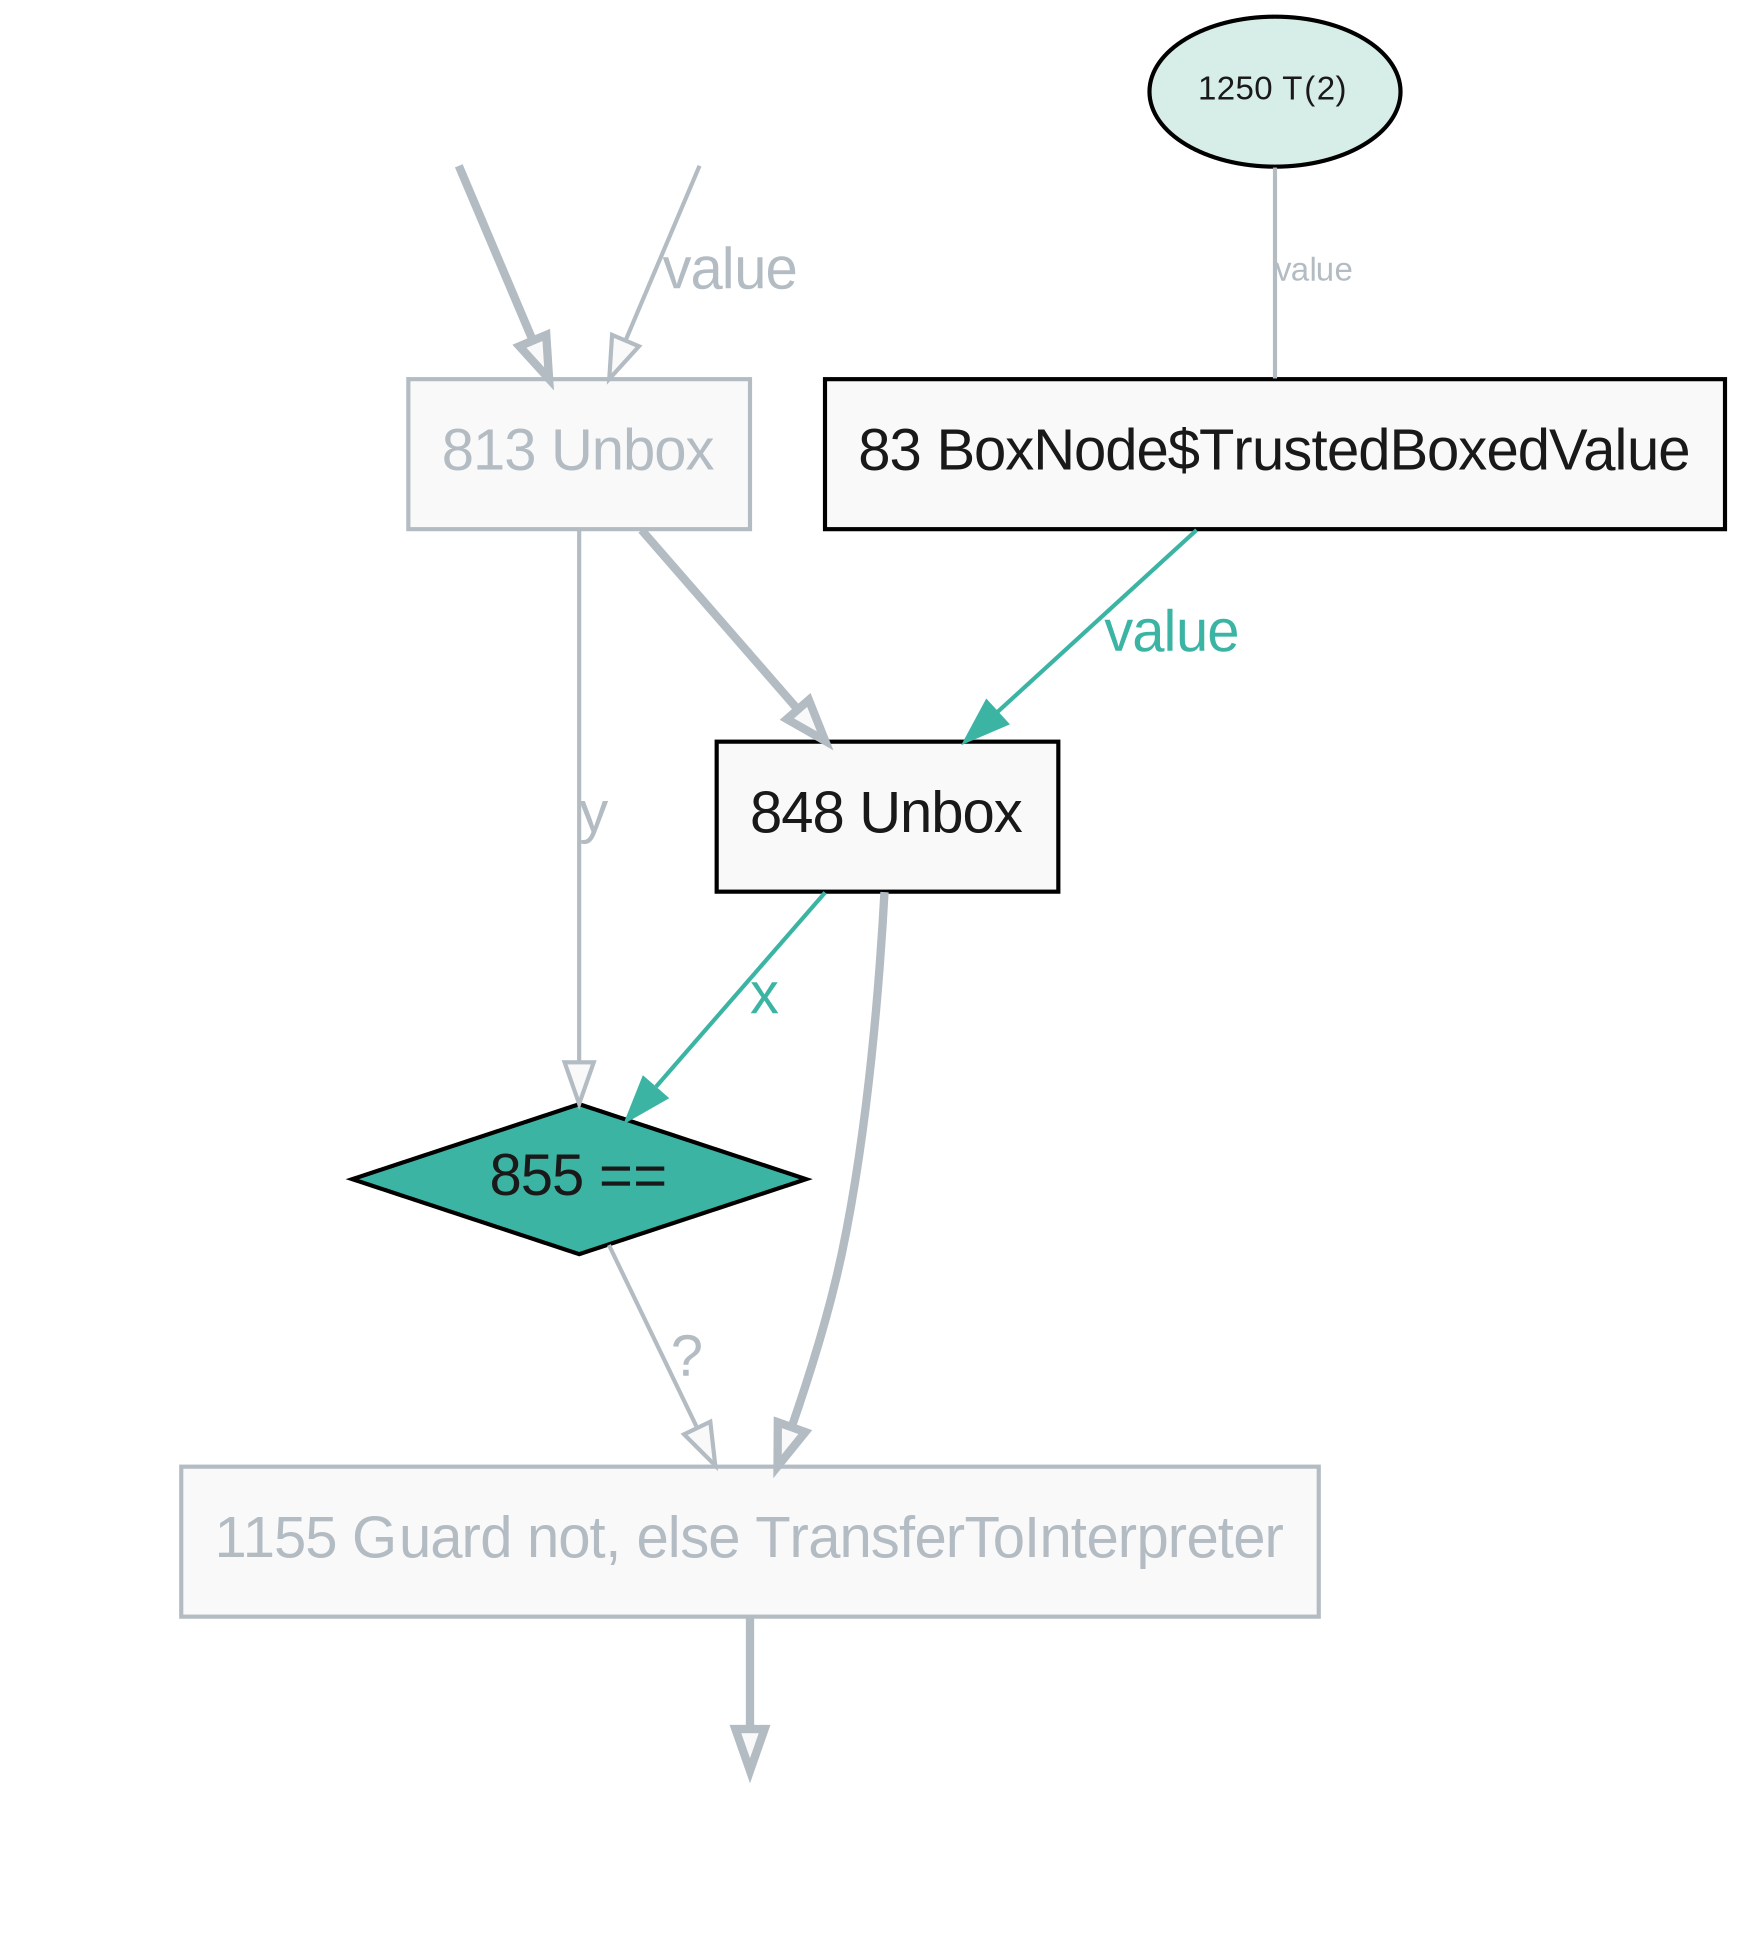
\includegraphics[width=0.4\textwidth]{figures/dot/List.contains.boxed-param-read.TruffleTier.png}
	\caption{Graal IR with speculative unboxing of \scalainline{elem} based on a type profile of its frame slot in \scalainline{List.contains}}
	\label{graalir:cons-contains-param-read}
\end{figure}

As previously mentioned, Truffle can speculatively optimize read operations on boxed frame values.
Figure \ref{graalir:cons-contains-param-read}, contains the parameter of \scalainline{elem} in \scalainline{List.contains}, which is an example of such a speculative optimization.
This speculative optimization relies on a \javainline{TrustedBoxedValue} to unbox the primitive.
A \javainline{TrustedBoxedValue} represents injected information from an external source.

In this particular case, it is known by the compiler that the boxed instance comes from the invocation \scalainline{List.contains((elem: Int))}.
Unique \javainline{int} values may be mapped to a unique \javainline{Integer} instance in the Java runtime, eliminating unnecessary boxed object creation.
The unbox operation in node $848$ will be `floated' up the graph such that all subsequent nodes dominated by the reading of a boxed frame value have no autoboxing.

This optimization is also possible because the invocation of \scalainline{contains} occurs in a single type context.
That is, \scalainline{contains} is only ever invoked with a single type argument in our microbenchmark; therefore, Truffle can insert speculative optimizations based on the type of the argument passed.
As the number of types is limited, in our case, only a single type, the value can be speculatively unboxed.
This optimization would \textit{not} be possible in a multiple type context, where \scalainline{contains} is invoked at many sites with distinct value type arguments.
This type of invocation environment, more commonly found in real-world programs, pollutes the type profiles of the method and inhibits speculative unboxing operations.
In theory, our approach to method specialization would not be hindered by this problem; we consider the evaluation of the interpreter in this environment out of the scope of this thesis.

\begin{figure}[!htb]
	\centering
	\begin{subfigure}[b]{0.4\textwidth}
		\centering
		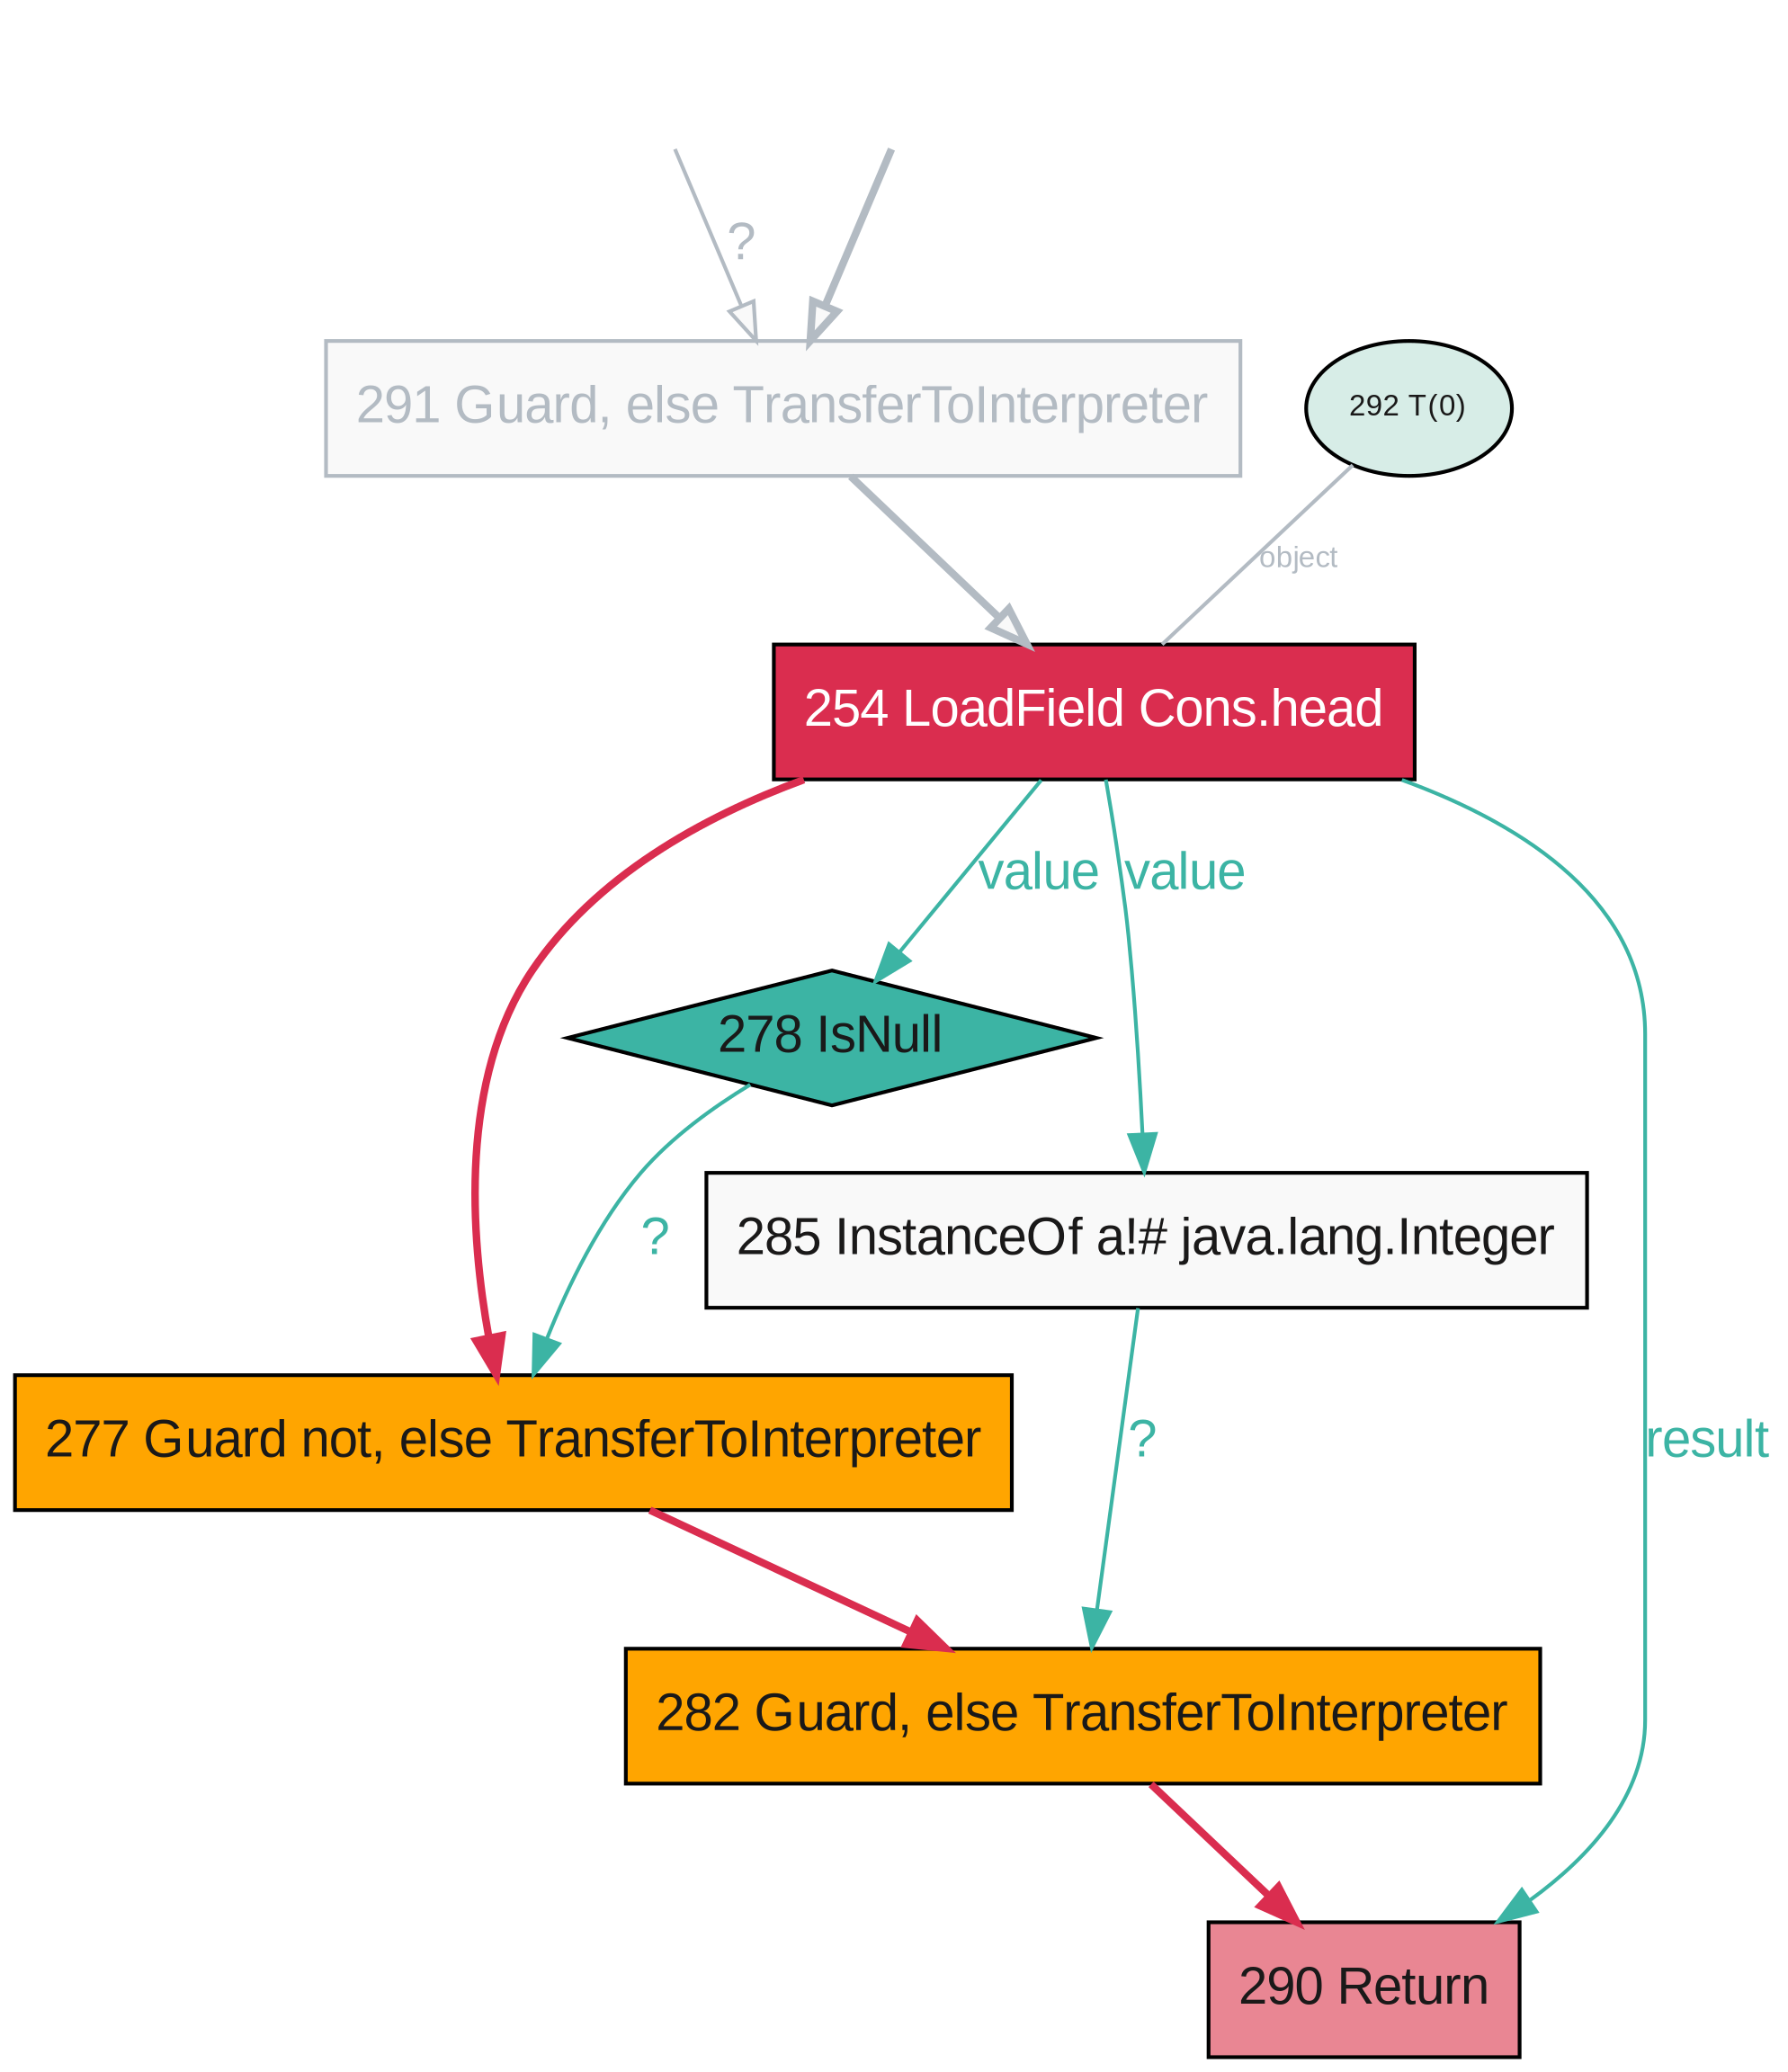
\includegraphics[width=\textwidth]{figures/dot/List.head.boxed.TruffleTier.png}
		\caption{Graal IR of \scalainline{Cons.head} focused on field access of \scalainline{head}}
		\label{graalir:cons-head-boxed}
	\end{subfigure}
	\hfill
	\begin{subfigure}[b]{0.45\textwidth}
		\centering
		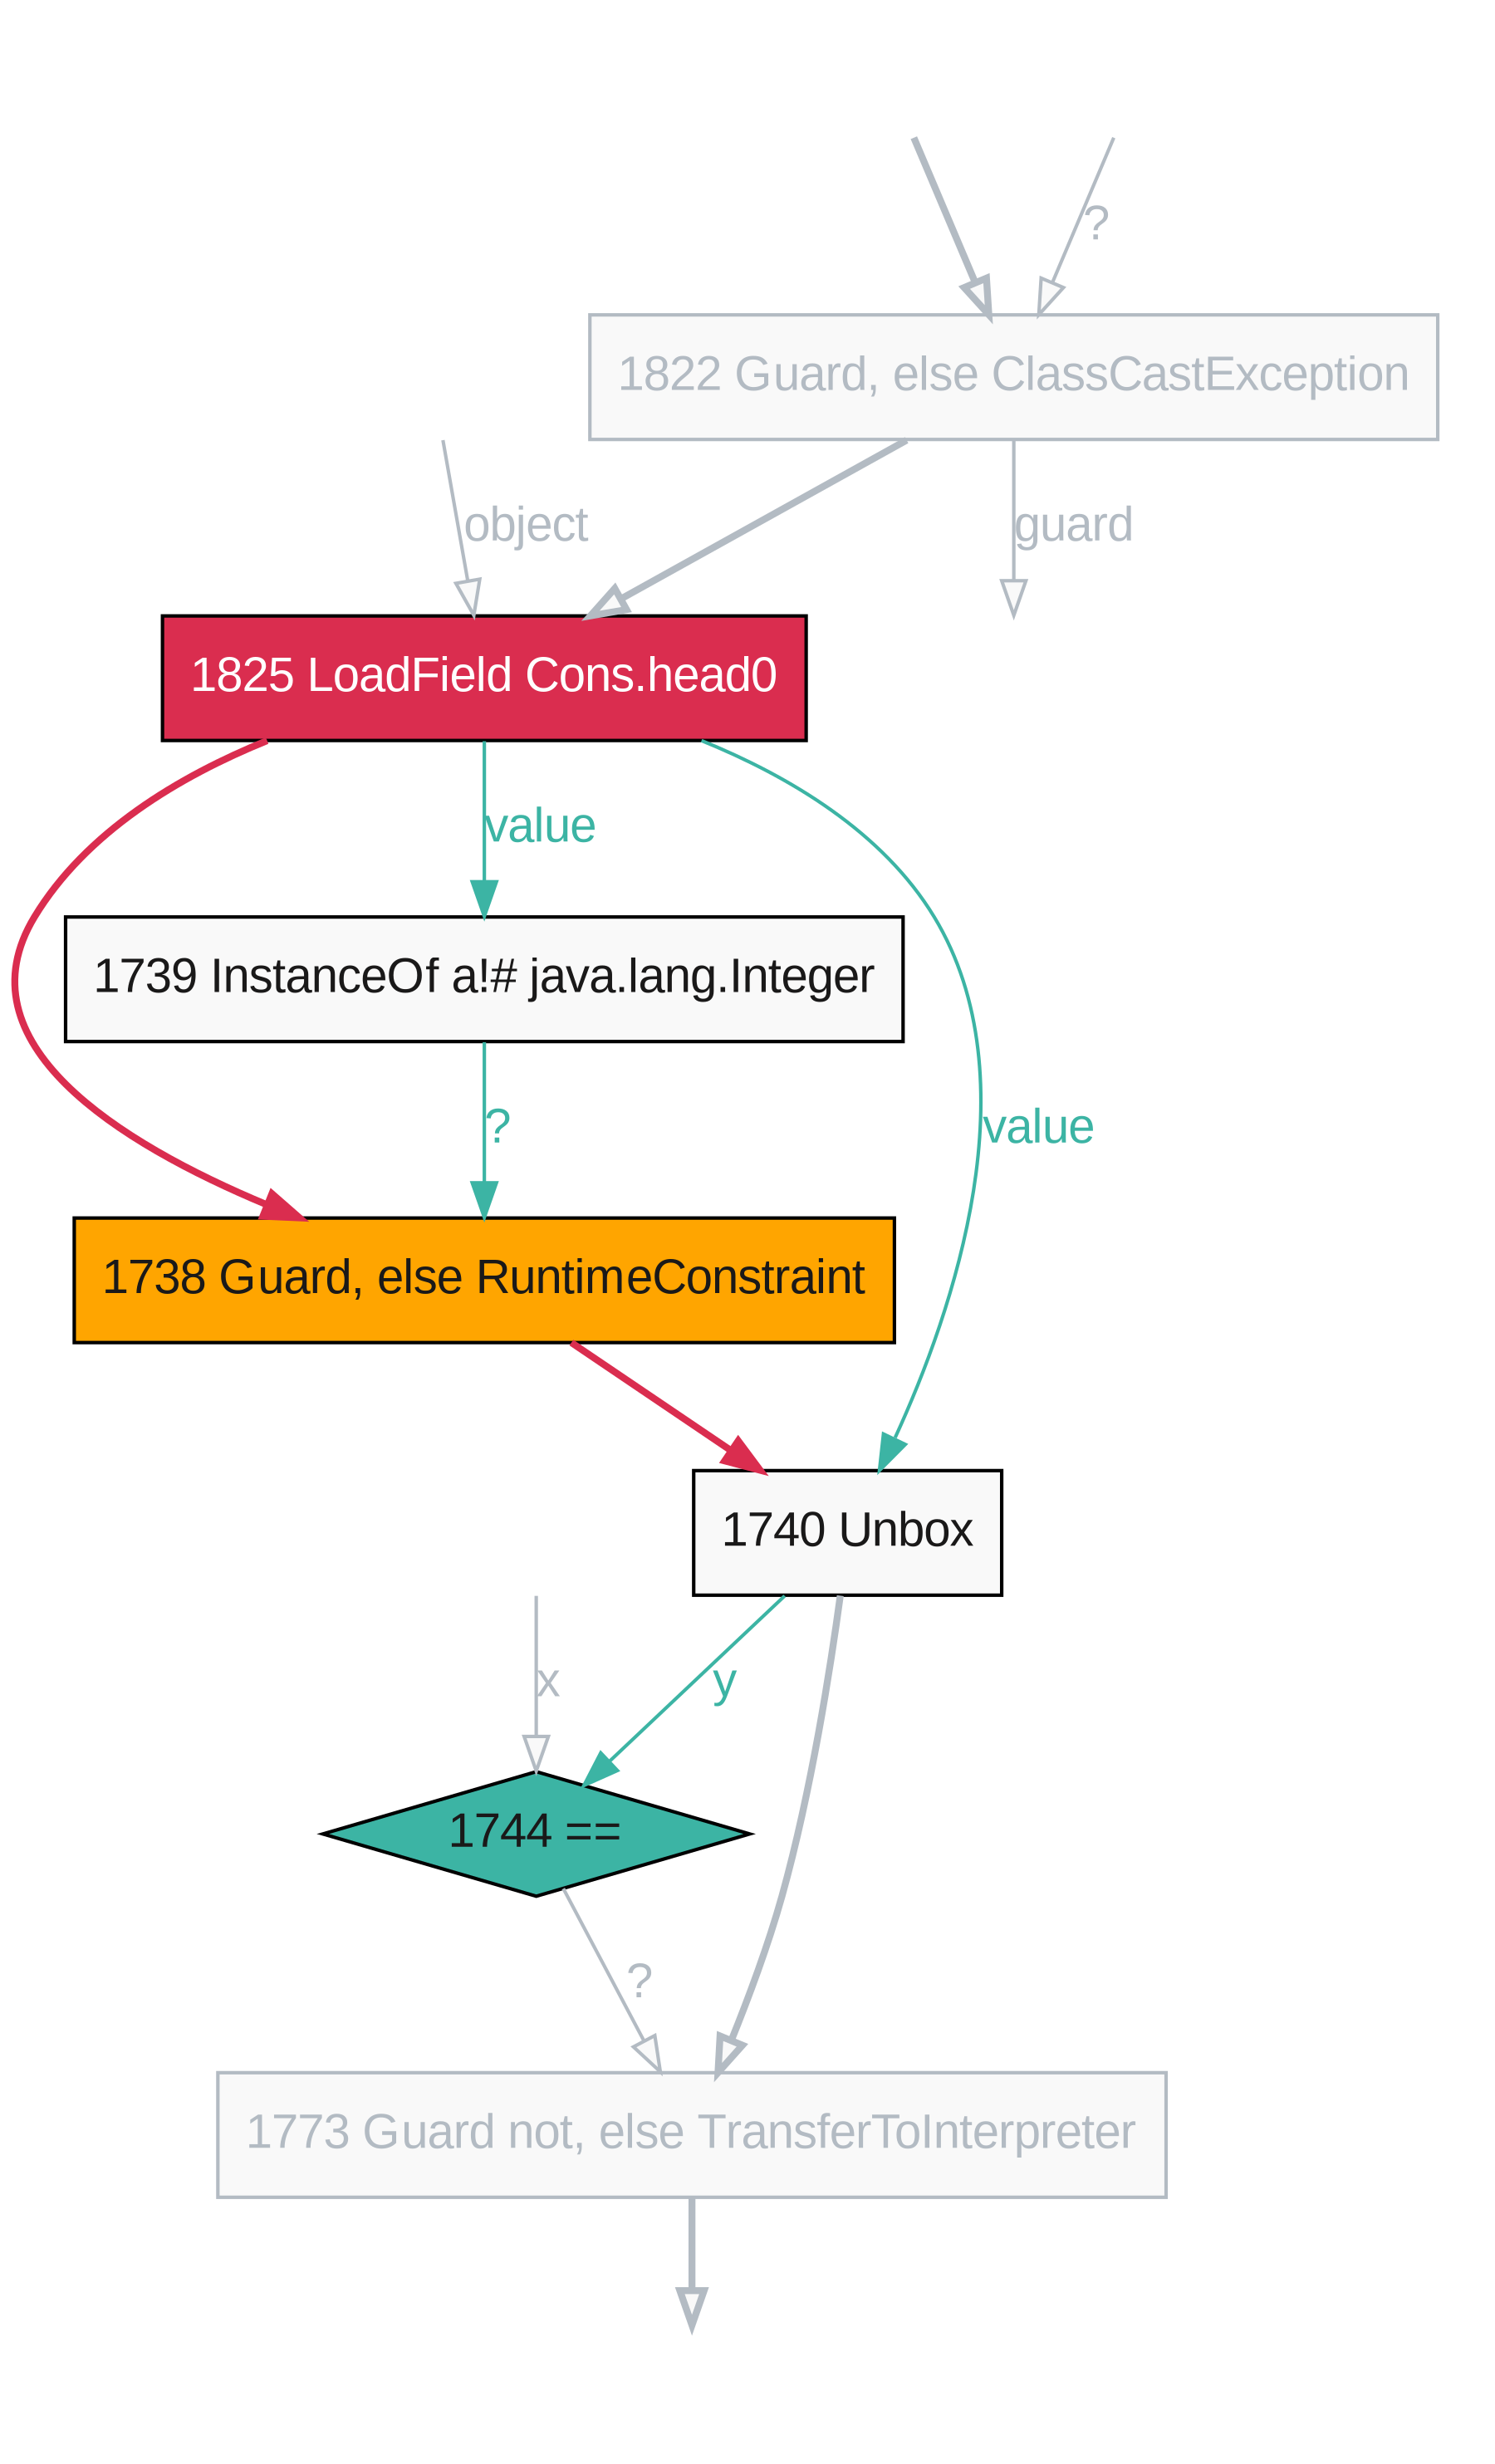
\includegraphics[width=\textwidth]{figures/dot/List.contains.boxed.TruffleTier.png}
		\caption{Graal IR of \scalainline{Cons.head} after being inlined into \scalainline{Cons.contains}}
		\label{graalir:cons-contains-head-focus-boxed}
	\end{subfigure}
	\hfill
	\caption{Comparison of Graal IR between unspecialized code of \scalainline{Cons.head} and specialized code of \scalainline{Cons.head} in the callee context.}
\end{figure}

We examine in detail the Graal IR focusing on the \scalainline{List.head} accessor method in our \scalainline{List} running example.
The accessor is frequently used in our \scalainline{List} microbenchmarks; Performance of \scalainline{List.contains} and \scalainline{List.hashCode} depends on the elimination of the unboxing in this method.
We focus on unboxing when the \scalainline{head} field is accessed by the \scalainline{List.head} accessor.
This unboxing can be seen in \ref{graalir:cons-head-boxed}.

We can see that \textit{guard} nodes are inserted by Graal into the compiled graph during JIT compilation.
A guard node ensures that a speculative assumption still holds during execution.
Because the default storage type of a polymorphic field without specialization is an \javainline{Object}, Graal makes two runtime assumptions about the field in the JIT compiled \scalainline{contains} method to ensure the compiled method does not throw a runtime exception if the return value needs to be unboxed.
The first guard, identifiable by node $278$, checks that the value is not the \javainline{null} reference.
As the \javainline{null} value is only compatible with reference types, attempting to unbox a \javainline{null} value produces a runtime exception.
The second guard, with the identifier $282$, is a type check that the value is an \javainline{Integer} object.
Notice that the predecessor node is the type check \javainline{instanceof a!{\#} java.lang.Integer} and not \javainline{instanceof java.lang.Integer}.
\javainline{instanceof} nodes in Graal IR checks against \textit{stamps} instead of normal JVM types identifiers.
A stamp is much like a type identifier but has additional descriptors attached.
For example, the stamp \javainline{a!{\#} java.lang.Integer} has the following descriptors:

\begin{description}
	\item[\texttt{(a)}] Asserts that the stamp marks a reference type identifier. The stamp marks the boxed reference type \javainline{java.lang.Integer}.
	\item[\texttt{(!)}] Asserts that the value is not the \javainline{null} reference value. The stamp contains this descriptor because it is preceded by a non-null guard.
	\item[\texttt{(\#)}] Asserts that the value marked by the stamp is \textit{exactly} an instance of the type identifier described by the stamp and not an instance of a subclass of the type identifier
\end{description}

In more succinct terms, the \javainline{instanceof} node $285$ checks that the value is precisely the instance of a \javainline{java.lang.Integer} and is not the \javainline{null} value. 
If the assumptions are not violated in compiled code, the boxed integer value is then returned from the compiled code.
Note that no unboxing happens because the value of \scalainline{head} has not yet been used in a polymorphic context.

\begin{figure}[!htb]
	\centering
	\begin{subfigure}[b]{0.4\textwidth}
		\centering
		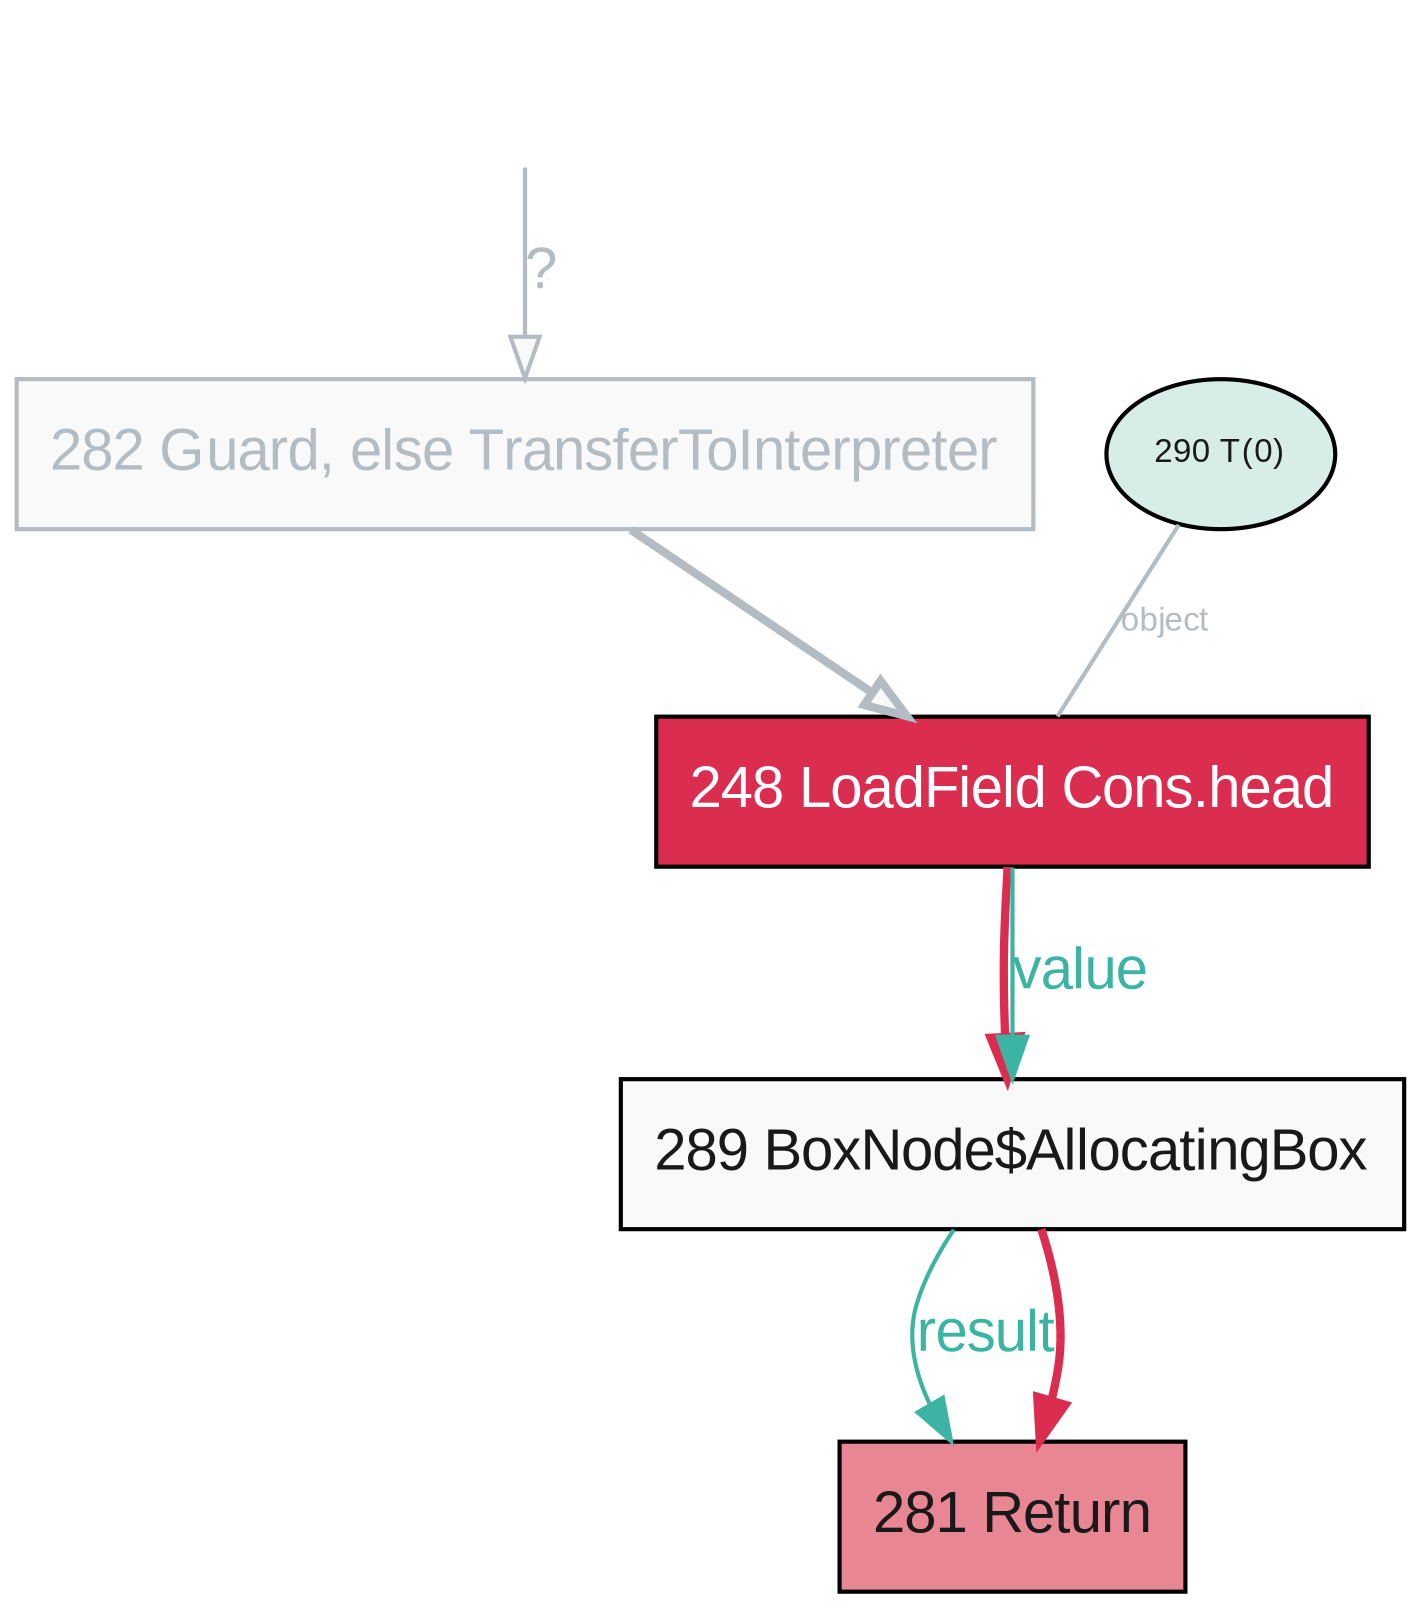
\includegraphics[width=\textwidth]{figures/dot/List.head.specialized.TruffleTier.png}
		\caption{Graal IR of \texttt{List.head} after field read of \texttt{head} is specialized.}
		\label{graalir:cons-head-specialized}
	\end{subfigure}
	\hfill
	\begin{subfigure}[b]{0.4\textwidth}
		\centering
		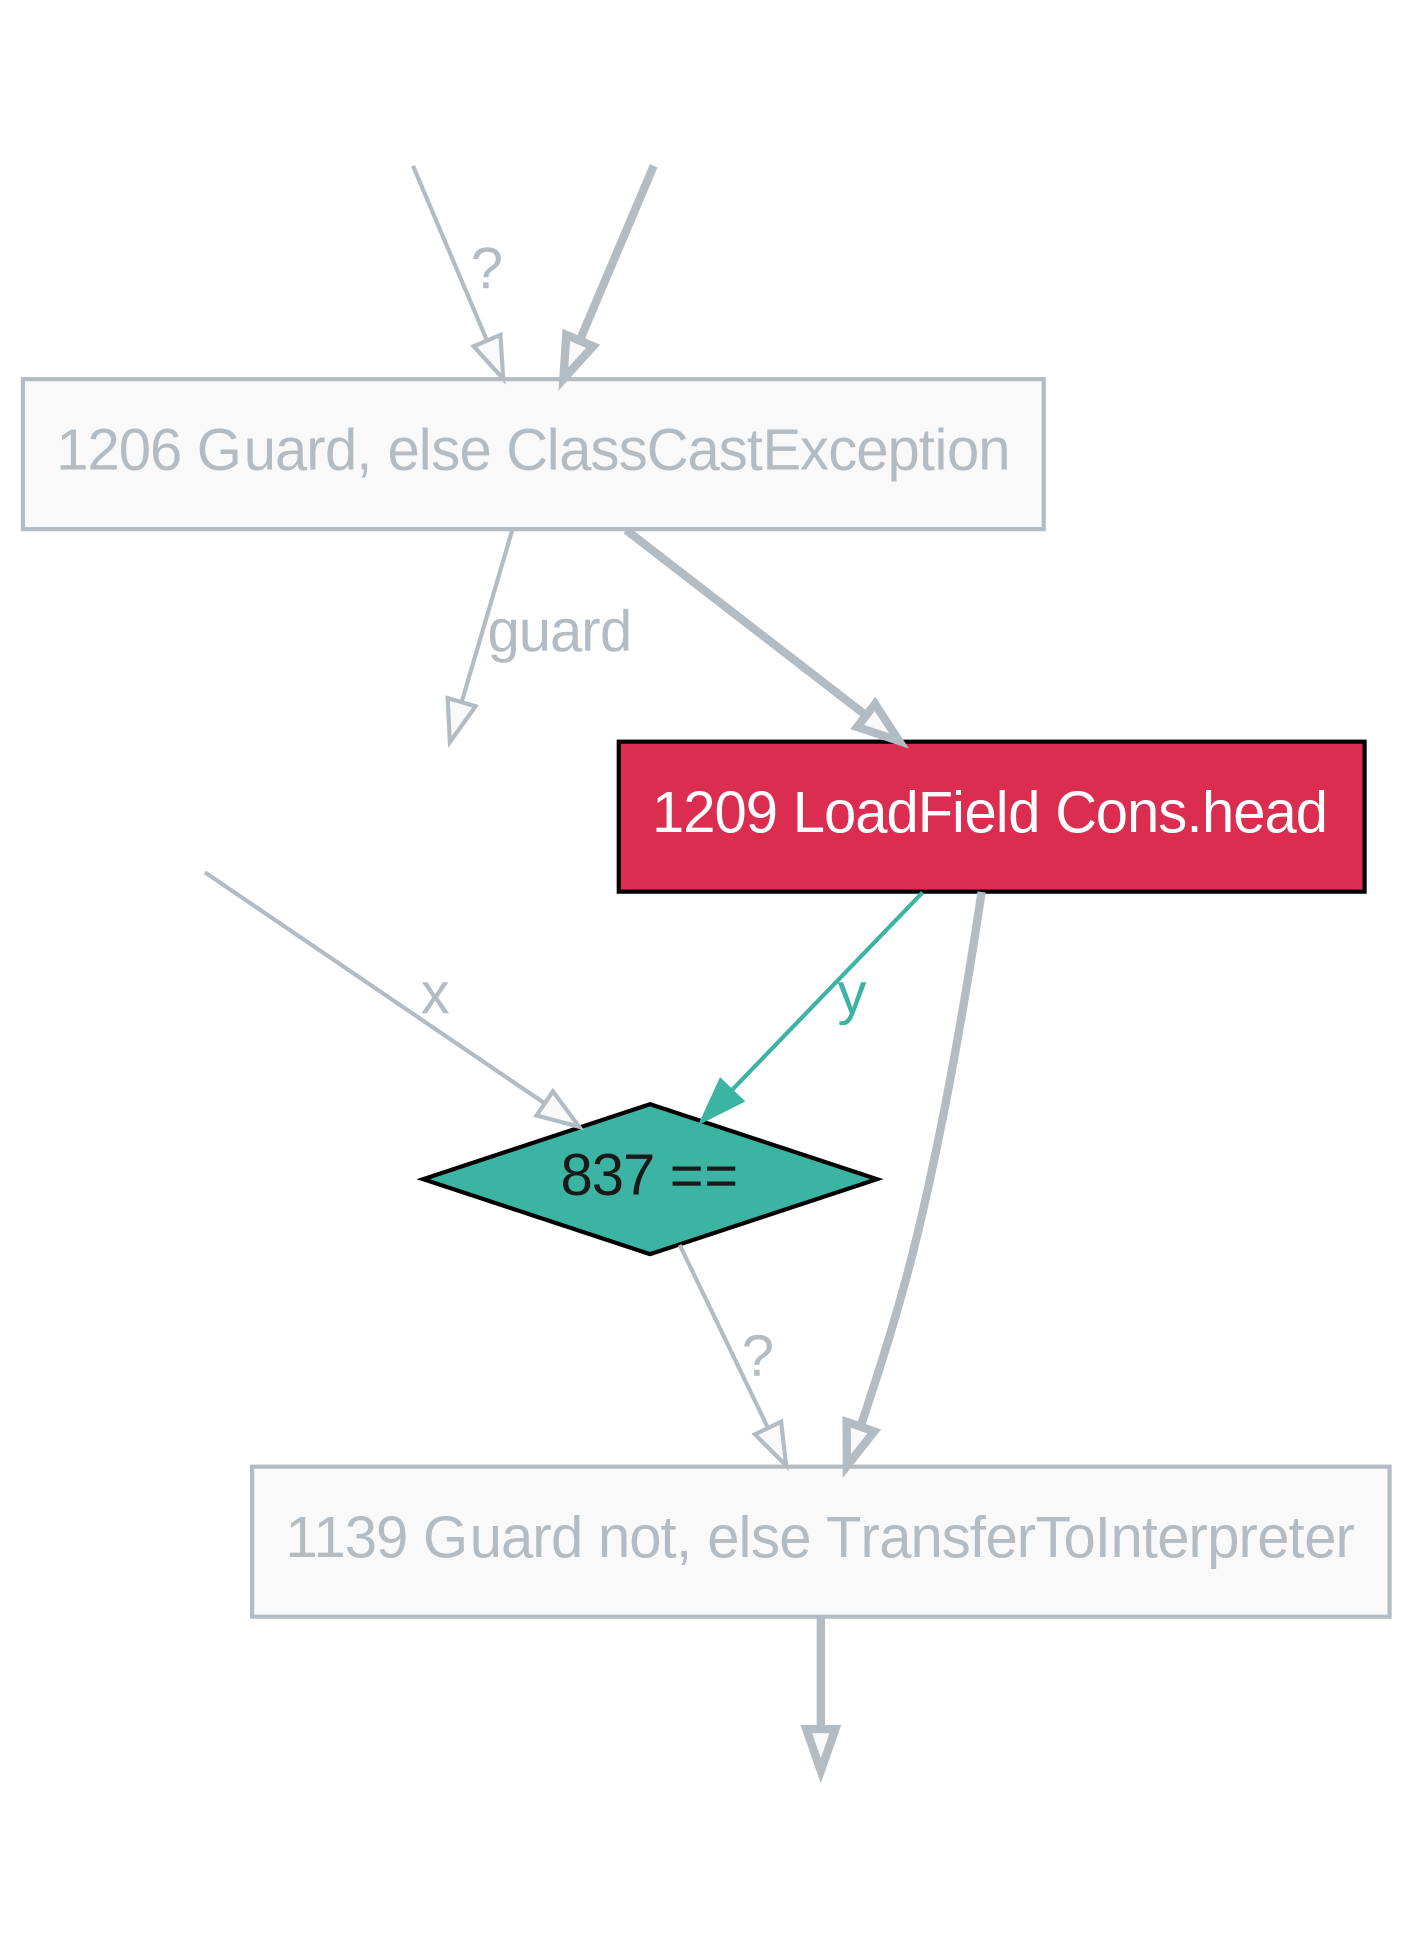
\includegraphics[width=\textwidth]{figures/dot/List.contains.specialized.TruffleTier.png}
		\caption{Graal IR of \scalainline{Cons.head} after being inlined into \scalainline{Cons.contains}}
		\label{graalir:cons-contains-head-focus-specialized}
	\end{subfigure}
	\hfill
	\caption{Comparison of Graal IR between unspecialized code of \scalainline{Cons.head} and specialized code of \scalainline{Cons.head} in the caller context.}
\end{figure}

When the access or method \scalainline{List.head} is inlined into its callsite in \scalainline{Cons.contains} (see figure \ref{graalir:cons-contains-head-focus-boxed}), an unbox operation is introduced because the equality operation in node $1744$ compares primitives and not references.
Notice that the two guard nodes previously seen in figure \ref{graalir:cons-head-boxed} are folded into one node because the \javainline{instanceof} node is an extension of the null check node.
Because polymorphic field values are stored as a reference on the object instance, these speculative assumptions are necessary to generate compiled code.
To eliminate the overhead of the unbox operation and the accompanying guard nodes, The polymorphic fields of a class must be specialized.

Figure \ref{graalir:cons-head-specialized} contains the field access of \scalainline{head} after the field has been specialized and has the appropriate storage type in the storage layout of \scalainline{Cons[Int]}.
Notice that a box node has been introduced prior to the value of \scalainline{head} prior to the return node of \scalainline{Cons.head}.
Because the \scalainline{execute} method of a \scalainline{DefDefNode} returns an \javainline{Object}, the return value is preemptively boxed when inspecting the IR of the method.
However, after inlining into the body of \scalainline{Cons.contains}, the box operation is no longer necessary as the boxed value will be immediately unboxed.
Graal will automatically eliminate this type of autoboxing.
When a specialized class instance is used in place of a generic class instance, the field access subgraph of \scalainline{List.head} is fully simplified.

\subsection{Mixing in Array Type Information}

While eliminating the autoboxing of frame and field accesses provided incremental improvements, incorporating array type information produced further throughput improvements for our array-backed microbenchmark.
In this section, we examine the Graal IR that contain type switches for the Scala runtime to handle arrays.

\begin{figure}[H]
	\centering
	\includegraphics[width=\textwidth]{figures/dot/List.apply.boxed.array_length.png}
	\caption{Graal IR of \scalainline{array_length} in the context of \scalainline{List.apply[T](array: Array[T])}}
	\label{graalir:list-apply-boxed-array-length}
\end{figure}

\begin{figure}[!htb]
	\centering
	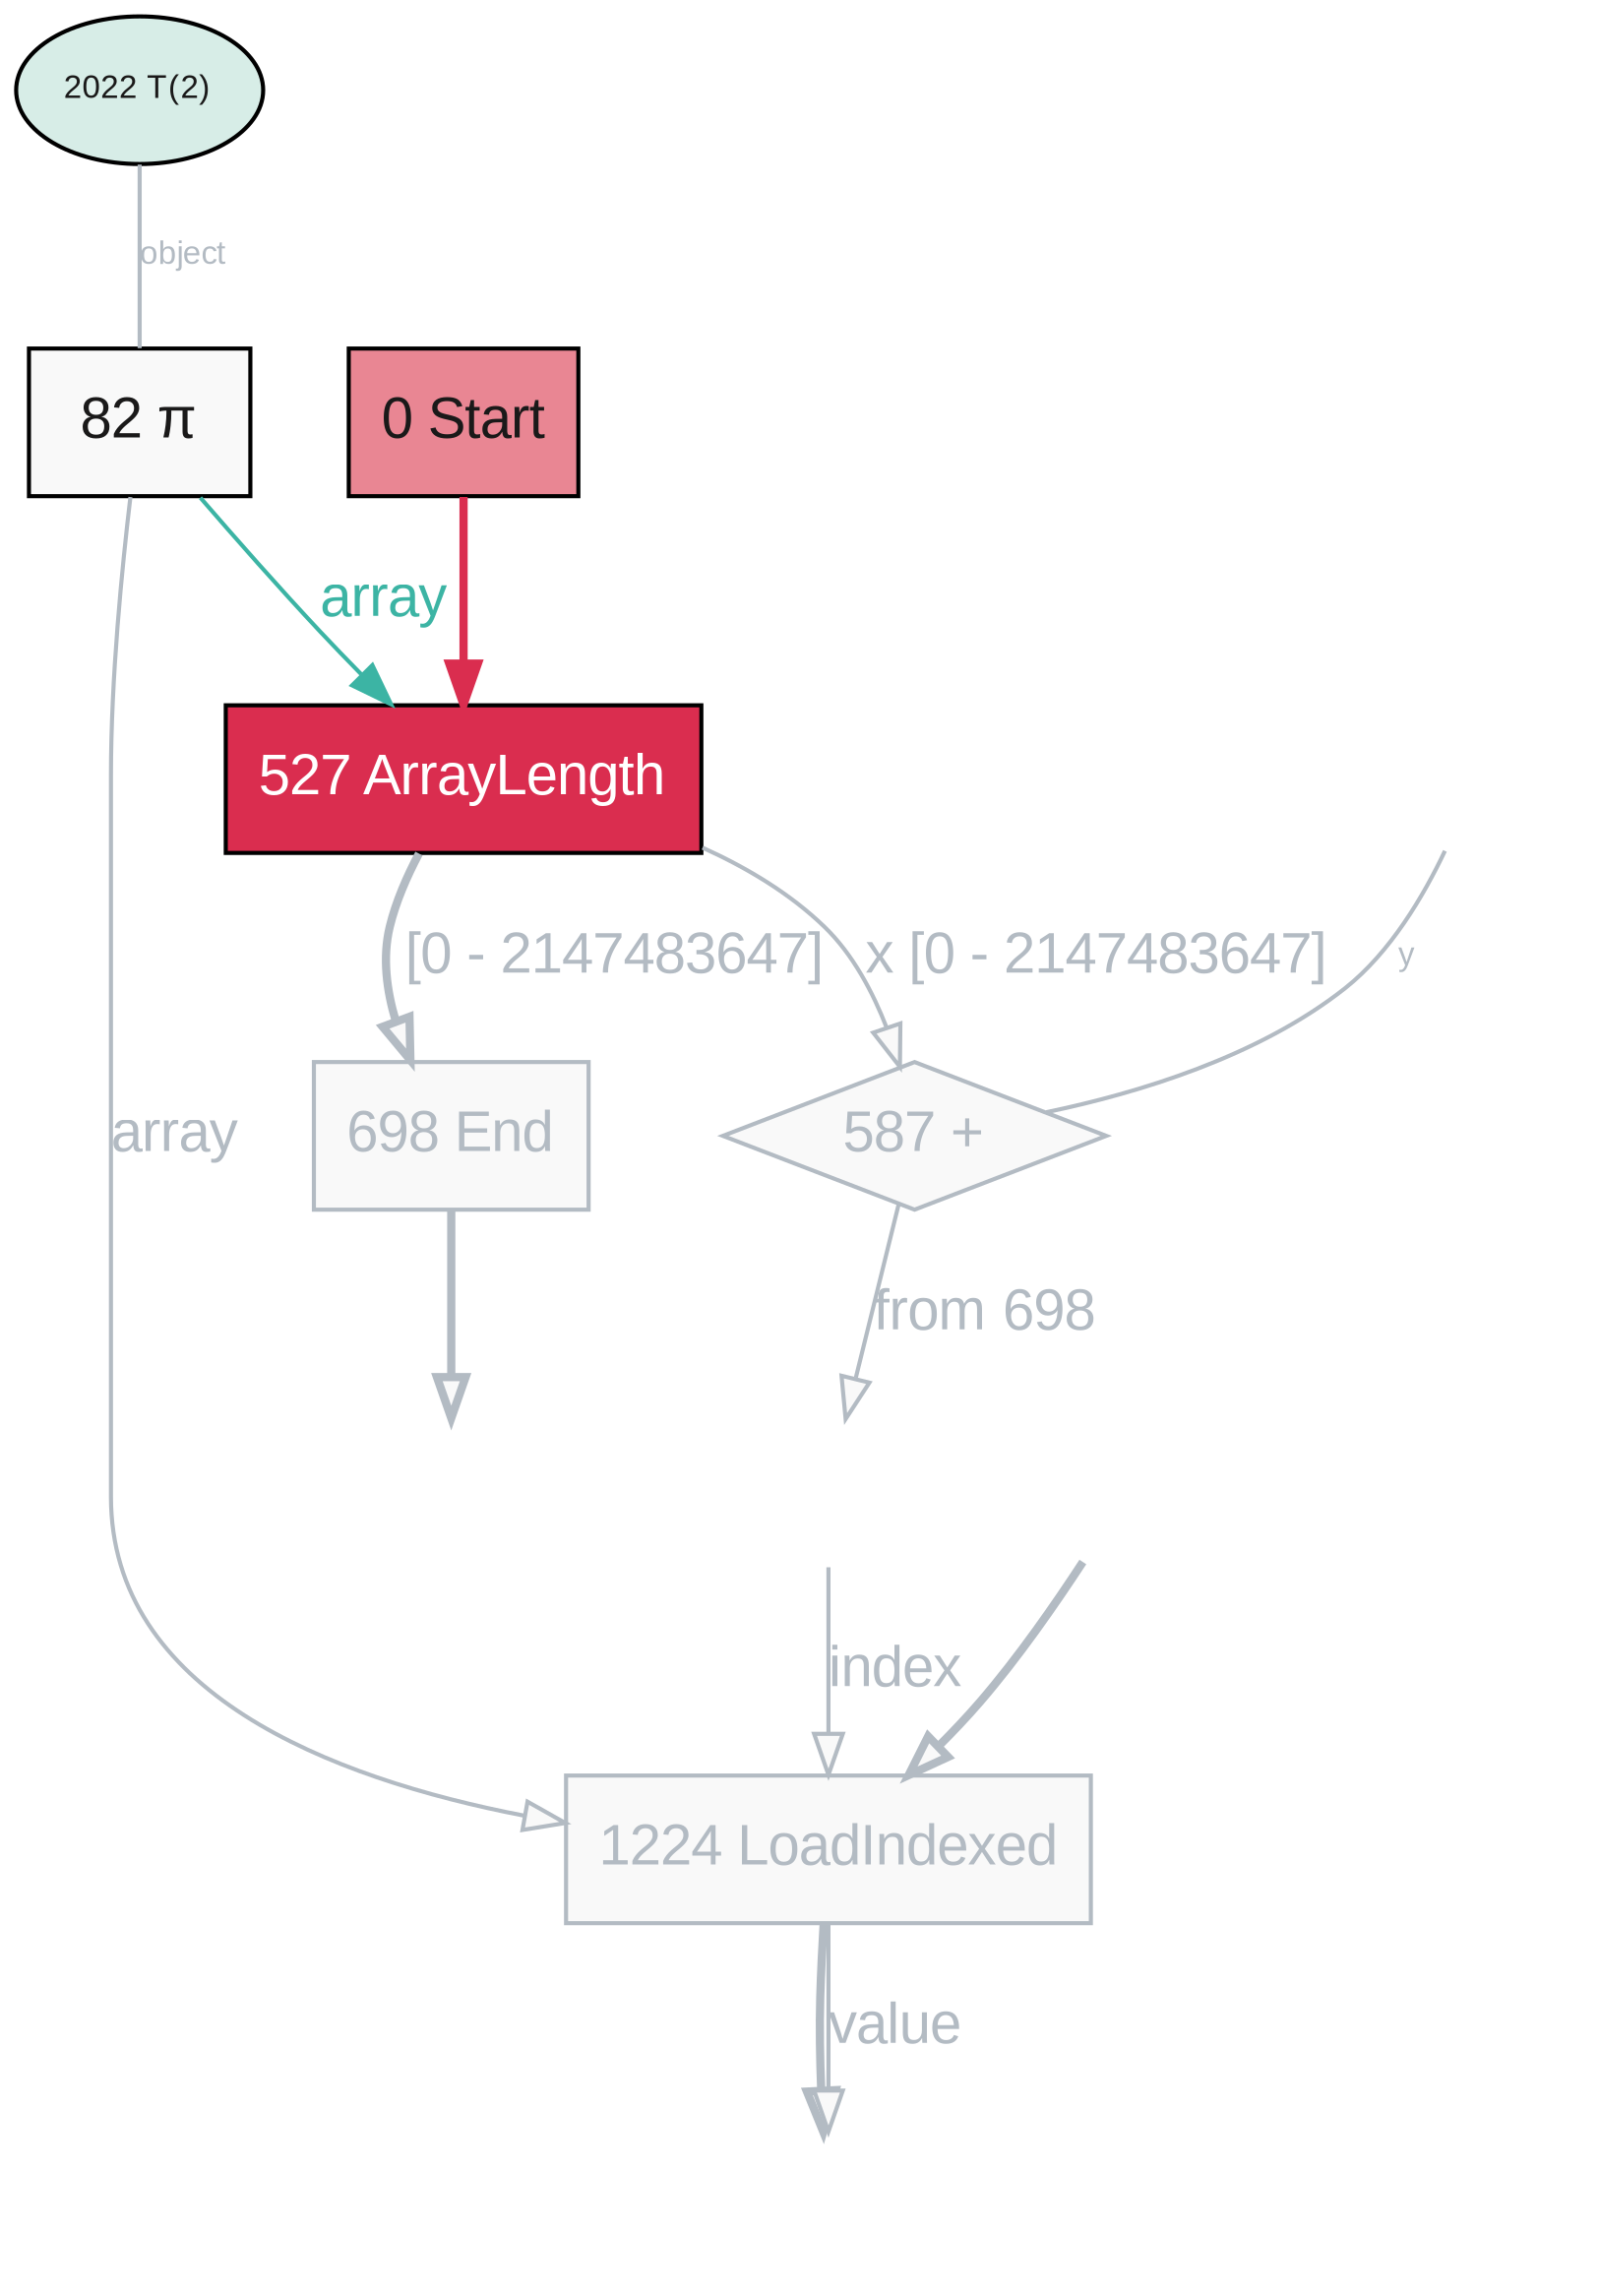
\includegraphics[width=0.3\textwidth]{figures/dot/List.apply.specialized.array_length.png}
	\caption{Graal IR of \scalainline{array_length} in the context of \scalainline{List.apply[T](array: Array[T])} augmented with a $\pi$ node}
	\label{graalir:list-apply-specialized-array-length}
\end{figure}

Figure \ref{graalir:list-apply-boxed-array-length} contains the Graal IR of \scalainline{array_length} inlined into \scalainline{List.apply[T]}. 
Notice that the \scalainline{instanceof} type checks nodes (white) that are succeeded by an \javainline{ArrayLength} node (red) for each of the branches in \scalainline{array_length}.
The numerous consecutive conditional expressions complicate the control flow analysis in JIT compilation.
These conditional checks add unnecessary branching and burdens JIT compilation when the type of a specialized array could be known from specialization.

Figure \ref{graalir:list-apply-specialized-array-length} contains the simplified Graal IR of \scalainline{array_length} inlined into \scalainline{List.apply[T]}.
Notice that there is a single \javainline{ArrayLength} node that is dominated by a $\pi$ node.
A $\pi$ node\cite{abdc:pi-nodes} enforces a bound on a value.
In the case of Graal, a $\pi$ node enforces a bound on the type of a value.
More specifically in our example, the $\pi$ node narrows the type of the 2nd parameter of \scalainline{List.apply[T]} to a monomorphic array type.
When the type of the parameter is narrowed, the type checks that enforce array types from figure \ref{graalir:list-apply-boxed-array-length} are eliminated because the type is now known.

This method does not consider polymorphic scenarios where an array of boxed primitives are used interchangeably with an array of primitives.
Such scenarios would require the insertion of additional autoboxing nodes or an intraprocedural transformation where boxed arrays are converted to primitive arrays.
While these solutions are possible in the context of Truffle, we consider these kinds of scenarios out of the scope of this thesis.




%======================================================================

\chapter{Related Work}

This chapter discusses previous academic and industrial work related to this thesis. 
The first section provides an introduction to the various implementations of parametric polymorphism.
The second section is a brief overview of programming languages that support a notion of reified types.
The third section covers related work on the implementation of polymorphism in Java.
The fourth section of this chapter provides an overview of previous and state-of-the-art efforts to specialize Scala programs.
The last section presents prior and ongoing efforts in the implementation of other Truffle interpreters.

\section{Implementations of Parametric Polymorphism}

Implementations of parametric polymorphism can be divided into two broad categories\cite{java:odersky-type-params}:

\begin{description}
	\item[\textit{Homogeneous Translation}] 
	This approach provides a single data representation for each polymorphic type. 
	An example of this implementation is the type erasure transformation applied in the Java and Scala compilation pipelines.
	Morrison et al. also refer to this form of polymorphism as the \textit{uniform polymorphism}\cite{napier88:polymorphism}.
	\item[\textit{Heterogeneous Translation}]
	In contrast to homogeneous translation, the heterogeneous translation ensures a unique data representation for every polymorphic type instantiation. The heterogeneous translation can also be referred to as \textit{textual polymorphism}.
\end{description}

This section will cover various approaches to implementing parametric polymorphism in the context of these two forms.
As polymorphism in Java and Scala are more relevant to the central themes of this thesis, we will first focus on implementations of parametric polymorphism for other languages.

Parametric polymorphism was first studied in functional programming languages\cite{ml:parametric-polymorphism,ml:type-inference}.
Leroy proposed an approach in which type coercion operations are inserted between polymorphic operations and monomorphic data. 
The coercion operations in this approach are quite similar to the notion of boxing and unboxing, which Leroy describes as \textit{wrapping} and \textit{unwrapping}.

The heterogeneous translation is a common implementation of parametric polymorphism in object-oriented programming languages.
\mintinline{cpp}|template| semantics in the \CC\ programming language popularized parametric polymorphism in objected-oriented programming languages.
Templates define a generic definition of some kind in \CC.
The \CC\ compiler will generate heterogeneous translations based on every set of concrete type arguments supplied during compilation.
The implementation of polymorphism in the Common Language Runtime\cite{clr:overview,clr:spec} by Kennedy and Syme makes use of reified types in a polymorphic bytecode IR during execution.
Polymorphic class definitions are loaded as templates; Templates generate specialized class layouts on an ad-hoc basis based on the reified type arguments seen during bytecode execution.
Their approach relies on CLR extensions to support types not present in existing JVM implementations.
Our approach shares many similarities with the approach described by Kennedy and Syme.
One drawback of their approach is that the polymorphic bytecode IR does not support the complete set of operations on types.
For an object instance of type \scalainline{List[T]}, it not possible to determine the concrete type of \scalainline{T}.
For example, reflection is necessary to differentiate between a \scalainline{List[Int]} and a \scalainline{List[String]}.
Furthermore, the authors note that their implementation is unable to support type variances, which are mainstays of the Scala type system, in their implementation of generics.
Our implementation differs as such operations are possible because the IR could potentially incorporate the full type language of TASTy.

\section{Implementations of Reified Types}

Some programming languages have previously introduced similar notions of types-as-values.
Zig\cite{zig} permits compilation-time types as first-class values. 
Compile-time evaluation in Zig exposes constant folding as a user abstraction.
Specific instantiations of generic data structures are then created based on reified type values during compilation-time.
Hack\cite{hack:inline-reified-types} and Kotlin\cite{kotlin:inline-functions} both have the notion of \textit{inline reified types}
More specifically, reified types in Hack and Zig allow type parameters of user-annotated inline-able methods to be available during run-time. 
Combined with inlining, this allows concrete type arguments from invocation sites to be used in the method body.
For example, run-time control flow based on concrete types are possible using inline reified types.
When combined with other higher-order abstractions, such as anonymous classes, inline reified types allow for data layout optimizations.

\section{Generics and Java}

Prior efforts to implement generics in Java have been based on static compilation techniques restricted by the \textit{open-world assumption}.
The open-world assumption is that the program under compilation is \textit{incomplete}; extra parts of the program will be supplied in a future iteration of compilation.
This form of compilation is commonly known as \textit{separate compilation}.
As such, the compilation results of the current parts of the program must be interoperable with the compilation results of the remaining yet-to-be-determined parts.

The Java language did not initially support parametric polymorphism.
As a result, many different approaches were proposed before a uniform polymorphism became the accepted implementation for Java.
Pizza\cite{java:pizza} was a superset of Java that supported heterogeneous and homogeneous translations of polymorphic definitions into Java.
Agesen, Freund, and Mitchell proposed a heterogeneous translation for parametric polymorphism for Java during load-time instead of compile-time\cite{java:agesen-type-params}.
NextGen\cite{java:nextgen} separates the translation of polymorphic classes into monomorphic and polymorphic components.
In NextGen, only the polymorphic members of a class definition are specialized; These specialized classes inherit the implementation of their monomorphic members from a common parent class.
Finally, GJ\cite{java:odersky-type-params} proposed the foundations for what is now the accepted implementation of parametric polymorphism in Java.
Polymorphic class definitions have a single uniform data representation after type erasure. these approaches determine the data representation of polymorphic definitions in a static context.
Our approach is based on the \textit{closed-world assumption}.

\section{Specialization in Scala}

The standard implementation of parametric polymorphism in Scala follows that of Java; generic class definitions have their type parameters erased.
All previous approaches attempt to avoid the problem of bytecode explosion, where the specialization of polymorphic data with every possible type creates an exponential number of unique data representations.
Dragos describes the earliest efforts to specialize Scala programs with the aid of annotations\cite{scala:specialization}.
Annotations avoid unnecessarily specializing polymorphic data through knowledge injected by a programmer.
Ureche, Talau, and Odersky expand upon this approach by reducing unnecessary duplication among specializations through sharing\cite{scala:miniboxing}.
Sharing exploits the insight that specializations of some value types may be reused for the specializations of other value types.
For example, the representation of \scalainline{ArrayBuffer[Long]} could be used, with the addition of some glue code, for the specialization of \scalainline{ArrayBuffer[Int]} instead of generating an additional specialized representation. 
Both approaches mix the implementation of uniform polymorphism with user-guided specialization directives.
Our approach generates a heterogeneous translation of a generic class definition on an ad-hoc basis.

\section{Truffle Interpreters}

There are many Truffle interpreters in active development at the time of writing.
TruffleRuby\cite{trufflyruby:specialization,truffleruby:object-model},FastR, Graal.js, Graal.Python,\cite{truffle:thesis} are some of the industrial implementations of dynamically typed languages implemented with Truffle.
They all make substantial use of Truffle facilities, some discussed earlier in this thesis, to speculative optimize program execution. 
Espresso\cite{graalvm:espresso} is an implementation of a Java bytecode interpreter in Truffle. 
Espresso is a metacircular implementation of a Java Virtual Machine.
Because Espresso executes the same Java bytecode format as other JVM implementations, it uses the same approaches to optimizing polymorphic data layout as the conventional implementation of Java on GraalVM.



%======================================================================
\chapter{Future Work}

TastyTruffle is intended to be a framework for dynamic whole-program approaches to optimizing Scala.
In this section, we discuss some possible extensions to the interpreter that further take advantage of Truffle mechanisms.
A substantial penalty of heterogeneous translations of polymorphic programs is \textit{code explosion}.
For large polymorphic programs, the penalty of heterogeneous translation is twofold.
The first is the cost of increased memory usage.
Having many specialized data representations incurs extra storage unless these data representations are regenerated every time a specialization is needed.
The second is the hidden computational overhead of specialization. 
Like other computational overheads of managed runtimes such as garbage collection, time spent generating specialized variants of polymorphic classes or methods means time not spent executing the program.
We propose several heuristics to influence \textit{when} a specialization is created.

Many prior approaches to specialization have already attempted to minimize the number of specializations to mitigate performance degradation for complex polymorphic definitions, where there is often a \(O(t^n)\) space complexity worse case\footnote{$t$ is the number of values types combined with the reference type, $n$ is the number of type parameters in a generic definition.}.
These approaches balance the tradeoff between performance and code size to optimistically generate \textit{only} the specializations required to eliminate performance bottlenecks.
Because of the work done in \cite{scala:specialization}, many existing Scala programs are already user-annotated with a specialization directive.
Similarly, our approach could be extended to include the semantics of this annotation, generating specializations with user-guide information only where needed.
The translation of non-annotated definitions will use a shared type-erased data representation.
However, mixing annotated and non-annotated programs will present missed optimization opportunities in the non-annotated portions of the program.

Truffle offers many mechanisms for profiling values and types.
Some of this profiling instrumentation is automatically done by Truffle, such as the profiling of argument types for node rewrites. In contrast, the guest language implementer adds other instrumentation,  such as condition profiles.
These profiles augment partial evaluation and enable speculative assumptions for optimizations such as conditional elimination.
We propose instrumenting specialization sites to profile type arguments.
Type argument profiles could then be used to decide the specific instantiation to specialize.
A \textit{profile-guided} approach to specialization could limit specializations to only the most frequently used instantiations.

Often a polymorphic instantiation is not sufficiently frequent to warrant specialization; the default homogeneous data representation will be shared among unspecialized instantiations.
A type-erased homogeneous data representation may still be tagged with the underlying applied type.
We can further augment type-erased polymorphic fields, and frame slots to profile reads from and writes to their respective storage locations.
These two pieces of dynamic information can be combined to allow the specialization of specific instantiations that are frequently manipulated but not frequently created.

We can apply the same optimization to sharing data layouts between specific specializations with inspiration from the work done by Ureche et al. in \cite{scala:miniboxing}.
Because the additional operations that adapt shared specializations to their original type contexts are negligible in terms of performance\cite{scala:miniboxing}, these operations make sense to implement directly as Truffle nodes that will be further optimized by JIT compilation.
%======================================================================
\chapter{Conclusions}

This thesis introduced \textsc{TastyTruffle}, a Truffle interpreter that is a platform for experimenting with ad hoc data representations.
The thesis described methods to translate TASTy, a tree serialization format for Scala 3, into an executable IR suitable for execution in an optimizing interpreter.
We show in this thesis how to exploit the type information present in an input source language such as TASTy to generate specialized data representations for polymorphic data structures.
We demonstrate that these techniques can substantially improve the performance of simple Scala programs in an experimental interpreter when compared to a state-of-the-art Java virtual machine.

A particular challenge in the implementation of \textsc{TastyTruffle} was the translation of TASTy into \textsc{TastyTruffle} IR.
Because TASTy is emitted after parsing and type checking, no other compiler transformations typical in other intermediate representations are present.
Many features of the Scala programming language are built as abstractions of simpler constructs that the compiler must further simplify.
Without the existing compiler transformations to simplify these abstractions, TASTy can be at times \textit{extraneously} high-level for execution.
While this did not significantly affect the evaluation of simple Scala programs for our experiments, it limits the \textit{breadth} of programs that are executable by our interpreter.
A possible solution to this hurdle is to read TASTy, perform a subset of Scala compiler transforms, then execute the program using our translation.
While we will have to avoid the type erasure transformation and all subsequent transformations that depend on the type erasure results, a much more significant portion of existing Scala programs can be executed on our interpreter. 
This capability is particularly important in the context of the Scala collections library. 
As many Scala applications rely extensively on the Scala collections library, it would open the possibility for evaluating \textsc{TastyTruffle} on larger real-world workloads.

The specialization of classes with both class-polymorphic and method-polymorphic semantics proved to be a complex implementation detail.
The gap between the specialization of classes (at object creation) and the specialization of methods (at method invocation) required the selection of appropriate intermediate representation to encapsulate the \textit{partial} specialization.
Partial specializations have been specialized but also still contain polymorphic semantics, which must be resolved at a future specialization site.
In this thesis, we chose to use a high-level approach to aid the translation of TASTy definitions with TASTy type arguments.
However, many prior approaches provide inspiration to tackle this problem.
A possible solution might avoid multiple mechanisms for specialization, there avoiding partial specializations entirely.
Alternatively, specialized call targets could be added onto a shape in an ad-hoc, profile-driven manner without the need to dispatch and select a specialization inside a call target.
Truffle already has the tooling for dynamic object layouts in the form of the \scalainline{DynamicShape}.
As class specialization is a relatively experimental feature in the lifespan of \textsc{TastyTruffle}, we consider this a possibility for future optimization.

In this thesis, we have evaluated \textsc{TastyTruffle} on simple but challenging to specialize data structures exhibiting bulk memory access and random heap access.
The elimination of autoboxing in the list data structure resulted in incremental performance improvements where autoboxing proved to be a performance bottleneck.
The elimination of autoboxing in data structures backed by polymorphic arrays resulted in performance improvements by an order of magnitude.
\textsc{TastyTruffle} validates that there are opportunities for data representation optimizations that bridge static compilation and just-in-time compilation.

%======================================================================

%----------------------------------------------------------------------
% END MATERIAL
%----------------------------------------------------------------------

% B I B L I O G R A P H Y
% -----------------------

% The following statement selects the style to use for references.  It controls the sort order of the entries in the bibliography and also the formatting for the in-text labels.
\bibliographystyle{plain}
% This specifies the location of the file containing the bibliographic information.  
% It assumes you're using BibTeX (if not, why not?).
\cleardoublepage % This is needed if the book class is used, to place the anchor in the correct page,
                 % because the bibliography will start on its own page.
                 % Use \clearpage instead if the document class uses the "oneside" argument
\phantomsection  % With hyperref package, enables hyperlinking from the table of contents to bibliography             
% The following statement causes the title "References" to be used for the bibliography section:
\renewcommand*{\bibname}{References}

% Add the References to the Table of Contents
\addcontentsline{toc}{chapter}{\textbf{References}}

\bibliography{uw-ethesis-mmath-jyou}
% Tip 5: You can create multiple .bib files to organize your references. 
% Just list them all in the \bibliogaphy command, separated by commas (no spaces).

% The following statement causes the specified references to be added to the bibliography% even if they were not 
% cited in the text. The asterisk is a wildcard that causes all entries in the bibliographic database to be included (optional).
\nocite{*}

% The \appendix statement indicates the beginning of the appendices.
\appendix
% Add a title page before the appendices and a line in the Table of Contents
\chapter*{APPENDICES}
\addcontentsline{toc}{chapter}{APPENDICES}

\chapter{Scala Unified Type System}
\includesvg[pretex=\footnotesize,width=\textwidth]{figures/svg/unified-types-diagram.svg}

\chapter{Scala 3 Compiler Phases}
\label{appendix:dotty-phases}
\begin{minted}{scala}
/** Phases dealing with the frontend up to trees ready for TASTY pickling */
protected def frontendPhases: List[List[Phase]] =
	// scanner, parser
	List(new Parser) ::     
	// namer, typer                  
	List(new TyperPhase) ::   
	// YCheck positions                
	List(new YCheckPositions) ::         
	// Sends information on classes' dependencies to sbt via callbacks 
	List(new sbt.ExtractDependencies) ::   
	// Extract info into .semanticdb files  
	List(new semanticdb.ExtractSemanticDB) :: 
	// Additional checks and cleanups after type checking
	List(new PostTyper) ::      
 // Additional checks and transformations for Scala.js (Scala.js only)              
	List(new sjs.PrepJSInterop) ::  
	// Check PCP, heal quoted types and expand macros         
	List(new Staging) ::      
	// Sends a representation of the API of classes to sbt via callbacks                
	List(new sbt.ExtractAPI) ::               
	// Set the `rootTreeOrProvider` on class symbols
	List(new SetRootTree) ::                  
	Nil

/** Phases dealing with TASTY tree pickling and unpickling */
protected def picklerPhases: List[List[Phase]] =
	List(new Pickler) ::            // Generate TASTY info
	List(new PickleQuotes) ::       // Turn quoted trees into explicit run-time data structures
	Nil

/** Phases dealing with the transformation from pickled trees to backend trees */
protected def transformPhases: List[List[Phase]] =
	List(
		// Some transformations to put trees into a canonical form
		new FirstTransform,
		// Internal use only: Check that compiled program has no data races involving global vars         
		new CheckReentrant,
		// Eliminate references to package prefixes in Select nodes         
		new ElimPackagePrefixes,    
		// Cook the comments: expand variables, doc, etc.
		new CookComments,         
	 // Check restrictions that apply to @static members  
		new CheckStatic,   
		// Reduce closure applications        
		new BetaReduce,      
		// Check initialization of objects       
		new init.Checker) ::        
	List(
		new ElimRepeated,           // Rewrite vararg parameters and arguments
		new ExpandSAMs,             // Expand single abstract method closures to anonymous classes
		new ProtectedAccessors,     // Add accessors for protected members
		new ExtensionMethods,       // Expand methods of value classes with extension methods
		new UncacheGivenAliases,    // Avoid caching RHS of simple parameterless given aliases
		new ByNameClosures,         // Expand arguments to by-name parameters to closures
		new HoistSuperArgs,         // Hoist complex arguments of supercalls to enclosing scope
		new SpecializeApplyMethods, // Adds specialized methods to FunctionN
		new RefChecks) ::           // Various checks mostly related to abstract members and overriding
	List(
	 	// Turn opaque into normal aliases
		new ElimOpaque,            
		// Compile cases in try/catch
		new TryCatchPatterns,      
		// Compile pattern matches
		new PatternMatcher,         
		// Make all JS classes explicit (Scala.js only)
		new sjs.ExplicitJSClasses,  
		// Add accessors to outer classes from nested ones.
		new ExplicitOuter,          
		// Make references to non-trivial self types explicit as casts
		new ExplicitSelf,           
		// Expand by-name parameter references
		new ElimByName,             
		// Optimizes raw and s string interpolators by rewriting them to string concatentations
		new StringInterpolatorOpt) :: 
	List(
	 	// Drop erased definitions from scopes and simplify erased expressions
		new PruneErasedDefs,
		// Remove placeholders of inlined patterns       
		new InlinePatterns,    
		// Inlines calls to value class methods     
		new VCInlineMethods,  
		// Express vararg arguments as arrays      
		new SeqLiterals, 
		// Special handling of `==`, `|=`, `getClass` methods           
		new InterceptedMethods, 
		// Replace non-private vals and vars with getter defs (fields are added later)    
		new Getters,
		// Specialized Function{0,1,2} by replacing super with specialized super                
		new SpecializeFunctions,  
		// Put try expressions that might execute on non-empty stacks into their own methods  
		new LiftTry, 
		// Collect fields that can be nulled out after use in lazy initialization               
		new CollectNullableFields,  
		// Expand outer selections
		new ElimOuterSelect,
		// Implement super accessors        
		new ResolveSuper,           
		// Add forwarders for FunctionXXL apply method
		new FunctionXXLForwarders,  
		// Add forwarders for aliases of superclass parameters
		new ParamForwarding,     
		// Optimize generic operations on tuples   
		new TupleOptimizations,   
		// Lift blocks from receivers of applications  
		new LetOverApply, 
		// Intercept creation of (non-generic) arrays and intrinsify.          
		new ArrayConstructors) ::  
	// Rewrite types to JVM model, erasing all type parameters, abstract types and refinements.	 
	List(new Erasure) ::            
	List(
		// Expand erased value types to their underlying implmementation types
		new ElimErasedValueType,    
		// Remove pure stats from blocks
		new PureStats,        
		// Peep-hole optimization to eliminate unnecessary value class allocations      
		new VCElideAllocations,   
		// Optimize `scala.Array.apply([....])` and `scala.Array.apply(..., [....])` into `[...]`  
		new ArrayApply,     
		// Adds fake new invocations to local JS classes in calls to `createLocalJSClass`        
		new sjs.AddLocalJSFakeNews, 
	 // Rewrite PolyFunction subclasses to FunctionN subclasses
		new ElimPolyFunction,     
	 // Rewrite tail recursion to loops 
		new TailRec,               
		// Fill in constructors for Java enums
		new CompleteJavaEnums,    
		// Expand trait fields and trait initializers  
		new Mixin,                  
		// Expand lazy vals
		new LazyVals,              
		// Add private fields to getters and setters
		new Memoize,                
	 // Expand non-local returns
		new NonLocalReturns,       
		// Represent vars captured by closures as heap objects
		new CapturedVars) ::        
	List(
		// Collect initialization code in primary constructors
		// Note: constructors changes decls in transformTemplate, 
		// no InfoTransformers should be added after it
		new Constructors,           
		// Count calls and allocations under -Yinstrument
		new Instrumentation) ::     
	List(
		// Lifts out nested functions to class scope, storing free variables in environments
		new LambdaLift,             
		// Note: in this mini-phase block scopes are incorrect. No phases that rely on scopes should be here
		// Replace `this` references to static objects by global identifiers
		new ElimStaticThis,         
		// Identify outer accessors that can be dropped
		new CountOuterAccesses) :: 
	List(
		// Drop unused outer accessors
		new DropOuterAccessors,     
		// Lift all inner classes to package scope
		new Flatten,                
		// Renames lifted classes to local numbering scheme
		new RenameLifted,           
		// Replace wildcards with default values
		new TransformWildcards,     
	 // Move static methods from companion to the class itself
		new MoveStatics,           
		// Widen private definitions accessed from nested classes
		new ExpandPrivate,          
	 // Repair scopes rendered invalid by moving definitions in prior phases of the group
		new RestoreScopes,         
		// get rid of selects that would be compiled into GetStatic
		new SelectStatic,           
		// Generate JUnit-specific bootstrapper classes for Scala.js (not enabled by default)
		new sjs.JUnitBootstrappers, 
		// Find classes that are called with super
		new CollectSuperCalls) ::   
	Nil
	
/** Generate the output of the compilation */
protected def backendPhases: List[List[Phase]] =
	List(new backend.sjs.GenSJSIR) :: // Generate .sjsir files for Scala.js (not enabled by default)
	List(new GenBCode) ::             // Generate JVM bytecode
	Nil
\end{minted}
%======================================================================

\end{document}
